\documentclass[KVasios-ECE-Dipl.-Thesis.tex]{subfiles} 
\begin{document}
\chapter{Μοντελοποίηση \& Έλεγχος Ρομποτικής Λαβής:\\Θεωρητικό Υπόβαθρο}
%\addcontentsline{toc}{chapter}{Εισαγωγή}
%Μελέτη της επίδρασης διαφόρων τεχνικών βελτιστοποίησης κώδικα που στοχεύουν στην αξιοποίηση της cache
%\apendix 
%\section{Μοντέλο Συστήματος}
%\addcontentsline{toc}{section}{Ρομποτική Επιστήμη}

Βασικός στόχος ενός ρομποτικού χεριού είναι ο χειρισμός αντικειμένων και στις 6 διαστάσεις. Στο παρελθόν πολλοί αλγόριθμοι
έχουν προταθεί βασιζόμενοι στην ψευδοαντίστροφη μήτρα της λαβής με κάποιο συντελεστή βάρους συνδυασμένοι με έλεγχο 
εσωτερικής δύναμης. Οι περισσότερες από αυτές τις μεθοδολογίες απαιτούν εύρωστη ανίχνευση/παρακολούθηση των επαφών καθώς
και διακοπτικούς ελεγκτές. Εισάγοντας την έννοια του \textit{εικονικού--αντικειμένου} (\textit{virtual--object}) έχουν αναπτυχθεί και αναφέρονται στη βιβλιογραφία τεχνικές ελέγχου ρομποτικής λαβής σε επίπεδο αντικειμένου (object--level)~\cite{WimboeckOttHirzinger2006,WimbockOttHinzinger2007,WimbockOttSchafferHirzinger}. Ο έλεγχος
παίρνει ως είσοδο το επιθυμητό πλαίσιο του αντικειμένου και τις επιθυμητές δυνάμεις λαβής. Ο έλεγχος σε επίπεδο αντικειμένου
έχει γενικά τα κάτωθι πλεονεκτήματα,
\begin{itemize}
\item Εύκολος ορισμός δυνάμεων λαβής ως αντιστάθμιση των αδρανειακών χαρακτηριστικών ρομπότ--αντικειμένου
\item Εύκολος ορισμός εξωτερικών δυνάμεων που δρουν στο αντικείμενο 
\item Αποφυγή αναίτιων μεγάλων εσωτερικών δυνάμεων
\end{itemize}
Ουσιαστικά ο στόχος της εργασίας αυτής είναι η δημιουργία εύρωστου και διαισθητικού νόμου ελέγχου για έλεγχο στο αντικείμενο
ο οποίος δεν απαιτεί εύρωστη ανίχνευση/παρακολούθηση των επαφών. 

\section{Μοντελοποίηση Ρομποτικού Χεριού}

Σε αυτή την ενότητα δομούνται διαδοχικά το κινηματικό, διαφορικό και δυναμικό μοντέλο του ρομποτικού χεριού.

\subsection{Κινηματικό Μοντέλο Ρομποτικού Χεριού}
\phantom{1}

\textbf{Ορθή Κινηματική Ανάλυση}
\\

Για την περιγραφή της θέσης και του προσανατολισμού μίας κινηματικής αλυσίδας η οποία αποτελείται από πρισματικές και στροφικές αρθρώσεις με τον ελάχιστο δυνατό αριθμό παραμέτρων ακολουθείται η μέθοδος Denavit--Hartenberg~\cite{G.TZAPHESTA:2003fk}. 
\begin{figure}[htbp]%  figure placement: here, top, bottom, or page
   		\centering
		%   \includegraphics[scale=0.6]{images_kefalaio3/denavit.pdf} 
   		\resizebox{0.4\textwidth}{!}{% Sketch output, version 0.2 (build 9, Thu Feb 8 22:06:23 2007)
% Output language: PGF/TikZ
% Sketch output, version 0.2 (build 9, Thu Feb 8 22:06:23 2007)
% Output language: PGF/TikZ
%\documentclass[12pt]{article}
%\usepackage[x11names,rgb]{xcolor}
%\usepackage{tikz}
%\usetikzlibrary{snakes}
%\usetikzlibrary{arrows}
%\usetikzlibrary{shapes}
%\usetikzlibrary{backgrounds}
%\usepackage{amsmath}
%%
%\usepackage[active,tightpage]{preview}
%\PreviewEnvironment{tikzpicture}
%\setlength\PreviewBorder{2pt}%
%
%\begin{document}

%\begin{pspicture}(-1,-1)(2,2)
%\pstVerb{1 setlinejoin}
%\psline(-1,-1)(.333,.333)
%\pspolygon[fillstyle=solid,fillcolor=white](0,0)(1,0)(0,1)
%\psline(.333,.333)(2,2)
%\end{pspicture}


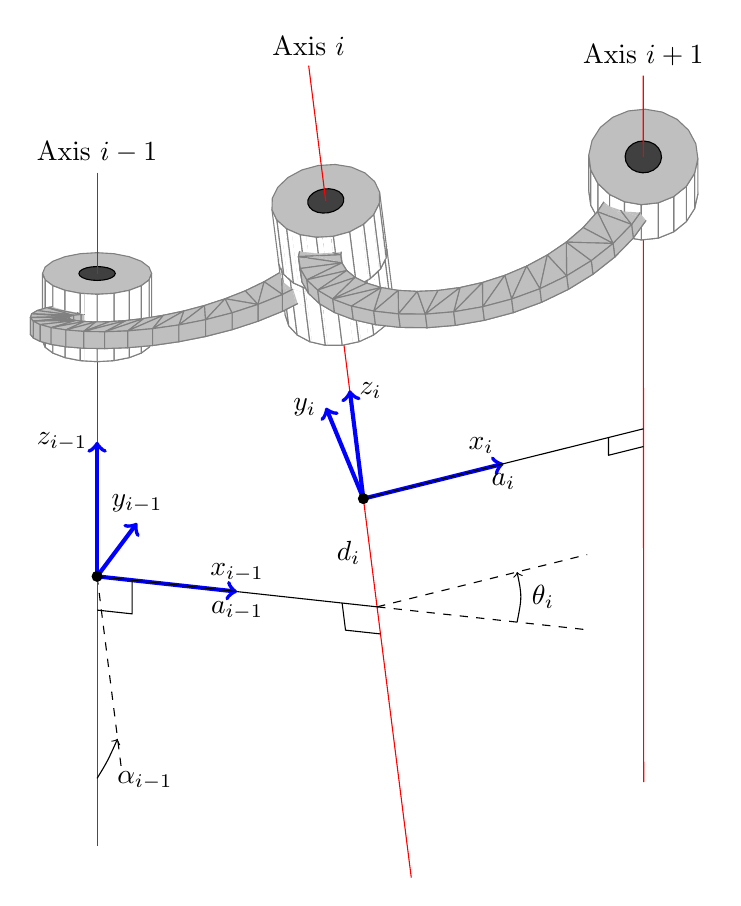
\begin{tikzpicture}[join=round]
\draw[draw=red](6.937,1.46)--(6.942,-6.031);
\draw[dashed](0,-3.419)--(.304,-5.825);
\draw[draw=red](3.078,-.026)--(3.99,-7.244);
\draw[arrows=<->,draw=blue,line width=1.5pt](1.778,-3.613)--(0,-3.419)--(.508,-2.742);
\draw[draw=red](0,-.427)--(0,-6.839);
\draw(.445,-3.468)--(.445,-3.895)--(0,-3.847);
\draw[arrows=->,draw=blue,line width=1.5pt](0,-3.419)--(0,-1.71);
\draw(0,-3.419)--(3.556,-3.806);
\draw(3.112,-3.758)--(3.155,-4.102)--(3.599,-4.15);
\draw[dashed](3.556,-3.806)--(6.224,-3.142);
\filldraw[fill=darkgray](-.187,-.376)--(-.136,-.356)--(-.072,-.344)--(0,-.339)--(.071,-.344)--(.136,-.356)--(.187,-.376)--(.22,-.4)--(.231,-.427)--(.22,-.455)--(.187,-.479)--(.136,-.499)--(.072,-.511)--(0,-.516)--(-.071,-.511)--(-.136,-.499)--(-.187,-.479)--(-.22,-.455)--(-.231,-.428)--(-.22,-.4)--cycle;
\filldraw[fill=lightgray,draw=gray](-.561,-.272)--(-.408,-.214)--(-.215,-.176)--(-.001,-.163)--(.214,-.176)--(.407,-.214)--(.561,-.272)--(.659,-.346)--(.693,-.427)--(.66,-.509)--(.561,-.583)--(.408,-.641)--(.215,-.679)--(.001,-.692)--(-.214,-.679)--(-.407,-.641)--(-.561,-.583)--(-.659,-.509)--(-.693,-.428)--(-.66,-.346)--cycle;
\draw[arrows=<->,draw=blue,line width=1.5pt](5.161,-1.989)--(3.382,-2.432)--(2.907,-1.277);
\draw[dashed](3.556,-3.806)--(6.223,-4.097);
\filldraw[fill=darkgray](0,-.339)--(0,.516)--(.071,.511)--(.071,-.344)--cycle;
\filldraw[fill=darkgray](-.072,-.344)--(-.072,.511)--(0,.516)--(0,-.339)--cycle;
\filldraw[fill=darkgray](.071,-.344)--(.071,.511)--(.136,.499)--(.136,-.356)--cycle;
\filldraw[fill=darkgray](-.136,-.356)--(-.136,.499)--(-.072,.511)--(-.072,-.344)--cycle;
\filldraw[fill=darkgray](.136,-.356)--(.136,.499)--(.187,.479)--(.187,-.376)--cycle;
\filldraw[fill=darkgray](-.187,-.376)--(-.187,.479)--(-.136,.499)--(-.136,-.356)--cycle;
\filldraw[fill=darkgray](.187,-.376)--(.187,.479)--(.22,.455)--(.22,-.4)--cycle;
\filldraw[fill=darkgray](-.22,-.4)--(-.22,.455)--(-.187,.479)--(-.187,-.376)--cycle;
\filldraw[fill=darkgray](.22,-.4)--(.22,.455)--(.231,.428)--(.231,-.427)--cycle;
\filldraw[fill=darkgray](.231,-.427)--(.231,.428)--(.22,.4)--(.22,-.455)--cycle;
\draw[draw=red](0,.427)--(0,-.427);
\filldraw[fill=darkgray,draw=none](-.231,-.428)--(-.231,-.184)--(-.22,-.174)--(-.22,-.4)--cycle;
\draw(-.22,-.174)--(-.22,-.4)--(-.231,-.428)--(-.231,-.184);
\filldraw[fill=darkgray,draw=none](-.231,-.184)--(-.231,.427)--(-.22,.455)--(-.22,-.174)--cycle;
\draw(-.231,-.184)--(-.231,.427)--(-.22,.455)--(-.22,-.174);
\filldraw[fill=darkgray](.22,-.455)--(.22,.4)--(.187,.376)--(.187,-.479)--cycle;
\filldraw[fill=darkgray](-.187,-.479)--(-.187,.376)--(-.22,.4)--(-.22,-.455)--cycle;
\filldraw[fill=darkgray,draw=none](-.22,-.222)--(-.22,.4)--(-.231,.427)--(-.231,-.211)--cycle;
\draw(-.22,-.222)--(-.22,.4)--(-.231,.427)--(-.231,-.211);
\filldraw[fill=darkgray](.187,-.479)--(.187,.376)--(.136,.356)--(.136,-.499)--cycle;
\filldraw[fill=darkgray](-.136,-.499)--(-.136,.356)--(-.187,.376)--(-.187,-.479)--cycle;
\filldraw[fill=darkgray](.136,-.499)--(.136,.356)--(.072,.344)--(.072,-.511)--cycle;
\filldraw[fill=darkgray](-.071,-.511)--(-.071,.344)--(-.136,.356)--(-.136,-.499)--cycle;
\filldraw[fill=darkgray](.072,-.511)--(.072,.344)--(0,.339)--(0,-.516)--cycle;
\filldraw[fill=darkgray](0,-.516)--(0,.339)--(-.071,.344)--(-.071,-.511)--cycle;
\filldraw[fill=lightgray,draw=gray](-.66,.509)--(-.693,.427)--(-.659,.346)--(-.561,.272)--(-.407,.214)--(-.214,.176)--(.001,.163)--(.215,.176)--(.408,.214)--(.561,.272)--(.66,.346)--(.693,.428)--(.659,.509)--(.561,.583)--(.407,.641)--(.214,.679)--(-.001,.692)--(-.215,.679)--(-.408,.641)--(-.561,.583)--cycle;
\filldraw[draw=gray,fill=white](.693,-.427)--(.693,.428)--(.66,.346)--(.66,-.509)--cycle;
\filldraw[fill=darkgray,draw=none](-.22,-.455)--(-.22,-.222)--(-.231,-.211)--(-.231,-.428)--cycle;
\draw(-.231,-.211)--(-.231,-.428)--(-.22,-.455)--(-.22,-.222);
\filldraw[draw=gray,fill=white](-.659,-.509)--(-.659,.346)--(-.693,.427)--(-.693,-.428)--cycle;
\draw(6.495,-1.656)--(6.495,-1.881)--(6.939,-1.77);
\filldraw[fill=darkgray](-.22,.455)--(-.231,.427)--(-.22,.4)--(-.187,.376)--(-.136,.356)--(-.071,.344)--(0,.339)--(.072,.344)--(.136,.356)--(.187,.376)--(.22,.4)--(.231,.428)--(.22,.455)--(.187,.479)--(.136,.499)--(.071,.511)--(0,.516)--(-.072,.511)--(-.136,.499)--(-.187,.479)--cycle;
\filldraw[draw=gray,fill=white](.66,-.509)--(.66,.346)--(.561,.272)--(.561,-.583)--cycle;
\filldraw[fill=lightgray,draw=none](-.255,-.285)--(-.407,-.256)--(-.561,-.213)--(-.568,-.21)--(-.47,-.195)--cycle;
\draw[draw=gray](-.568,-.21)--(-.47,-.195)--(-.255,-.285);
\filldraw[fill=lightgray,draw=none](-.568,.004)--(-.568,-.21)--(-.47,-.195)--(-.47,.019)--cycle;
\draw[draw=gray](-.568,-.21)--(-.47,-.195)--(-.47,.019)--(-.568,.004);
\filldraw[fill=lightgray,draw=none](-.255,-.071)--(-.407,-.042)--(-.561,.001)--(-.568,.004)--(-.47,.019)--cycle;
\draw[draw=gray](-.568,.004)--(-.47,.019)--(-.255,-.071);
\filldraw[draw=gray,fill=white](-.561,-.583)--(-.561,.272)--(-.659,.346)--(-.659,-.509)--cycle;
\filldraw[draw=none,fill=white](-.214,-.679)--(-.214,-.296)--(-.255,-.285)--(-.407,-.256)--(-.407,-.641)--cycle;
\draw[draw=gray](-.407,-.256)--(-.407,-.641)--(-.214,-.679)--(-.214,-.296);
\filldraw[draw=none,fill=white](-.163,-.682)--(-.163,-.306)--(-.214,-.298)--(-.214,-.679)--cycle;
\draw[draw=gray](-.214,-.298)--(-.214,-.679)--(-.163,-.682);
\filldraw[draw=none,fill=white](-.163,-.306)--(-.214,-.296)--(-.214,-.298)--cycle;
\draw[draw=gray](-.214,-.296)--(-.214,-.298);
\filldraw[fill=lightgray,draw=gray](-.47,-.195)--(-.073,-.304)--(-.204,-.307)--cycle;
\draw[draw=red](0,1.71)--(0,.427);
\filldraw[draw=gray,fill=white](.561,-.583)--(.561,.272)--(.408,.214)--(.408,-.641)--cycle;
\filldraw[fill=lightgray,draw=none](-.214,-.082)--(-.255,-.071)--(-.47,.019)--(-.073,-.09)--(-.163,-.092)--cycle;
\draw[draw=gray](-.255,-.071)--(-.47,.019)--(-.073,-.09)--(-.163,-.092);
\filldraw[draw=gray,fill=white](-.407,-.641)--(-.407,.214)--(-.561,.272)--(-.561,-.583)--cycle;
\draw(3.382,-2.432)--(6.939,-1.545);
\filldraw[fill=lightgray,draw=none](-.561,-.213)--(-.571,-.21)--(-.568,-.21)--cycle;
\draw[draw=gray](-.571,-.21)--(-.568,-.21);
\filldraw[fill=lightgray,draw=none](-.568,.004)--(-.639,-.007)--(-.639,-.221)--(-.568,-.21)--cycle;
\draw[draw=gray](-.568,.004)--(-.639,-.007)--(-.639,-.221)--(-.568,-.21);
\filldraw[draw=gray,fill=white](.408,-.641)--(.408,.214)--(.215,.176)--(.215,-.679)--cycle;
\filldraw[fill=lightgray,draw=none](-.561,-.213)--(-.462,-.256)--(-.639,-.221)--(-.571,-.21)--cycle;
\draw[draw=gray](-.462,-.256)--(-.639,-.221)--(-.571,-.21);
\filldraw[fill=lightgray,draw=none](-.263,-.295)--(-.462,-.256)--(-.561,-.213)--cycle;
\draw[draw=gray](-.263,-.295)--(-.462,-.256);
\filldraw[fill=lightgray,draw=none](-.561,.001)--(-.571,.004)--(-.568,.004)--cycle;
\draw[draw=gray](-.571,.004)--(-.568,.004);
\filldraw[fill=lightgray,draw=none](-.561,.001)--(-.462,-.042)--(-.639,-.007)--(-.571,.004)--cycle;
\draw[draw=gray](-.462,-.042)--(-.639,-.007)--(-.571,.004);
\filldraw[draw=gray,fill=white](.215,-.679)--(.215,.176)--(.001,.163)--(.001,-.692)--cycle;
\filldraw[draw=none,fill=white](-.163,-.306)--(-.163,-.092)--(-.214,-.084)--(-.214,-.296)--cycle;
\draw[draw=gray](-.214,-.084)--(-.214,-.296);
\filldraw[fill=lightgray,draw=gray](-.204,-.093)--(-.204,-.307)--(-.073,-.304)--(-.073,-.091)--cycle;
\filldraw[draw=none,fill=white](-.163,-.682)--(.001,-.692)--(.001,-.34)--(-.163,-.306)--cycle;
\draw[draw=gray](-.163,-.682)--(.001,-.692)--(.001,-.34);
\filldraw[draw=none,fill=white](-.214,-.296)--(-.214,-.08)--(-.407,-.042)--(-.407,-.247)--cycle;
\draw[draw=gray](-.214,-.296)--(-.214,-.08);
\draw[draw=gray](-.407,-.042)--(-.407,-.247);
\filldraw[fill=lightgray,draw=none](-.263,-.081)--(-.462,-.042)--(-.561,.001)--cycle;
\draw[draw=gray](-.263,-.081)--(-.462,-.042);
\filldraw[fill=lightgray,draw=none](-.639,-.221)--(-.462,-.256)--(-.287,-.315)--(-.298,-.317)--cycle;
\draw[draw=gray](-.287,-.315)--(-.298,-.317)--(-.639,-.221)--(-.462,-.256);
\filldraw[fill=lightgray,draw=gray](-.298,-.317)--(-.76,-.256)--(-.639,-.221)--cycle;
\filldraw[fill=lightgray,draw=gray](-.76,-.043)--(-.76,-.256)--(-.639,-.221)--(-.639,-.007)--cycle;
\filldraw[fill=lightgray,draw=none](-.255,-.285)--(-.204,-.307)--(-.263,-.295)--(-.407,-.256)--cycle;
\draw[draw=gray](-.255,-.285)--(-.204,-.307)--(-.263,-.295);
\filldraw[draw=none,fill=white](-.255,-.285)--(-.407,-.247)--(-.407,-.256)--cycle;
\draw[draw=gray](-.407,-.247)--(-.407,-.256);
\filldraw[fill=lightgray,draw=none](-.462,-.256)--(-.263,-.295)--(-.212,-.308)--(-.287,-.315)--cycle;
\draw[draw=gray](-.462,-.256)--(-.263,-.295);
\draw[draw=gray](-.212,-.308)--(-.287,-.315);
\filldraw[fill=lightgray,draw=none](-.639,-.007)--(-.462,-.042)--(-.287,-.102)--(-.298,-.103)--cycle;
\draw[draw=gray](-.287,-.102)--(-.298,-.103)--(-.639,-.007)--(-.462,-.042);
\filldraw[fill=lightgray,draw=gray](-.298,-.103)--(-.76,-.043)--(-.639,-.007)--cycle;
\filldraw[draw=none,fill=white](-.214,-.08)--(-.214,.176)--(-.407,.214)--(-.407,-.042)--cycle;
\draw[draw=gray](-.214,-.08)--(-.214,.176)--(-.407,.214)--(-.407,-.042);
\filldraw[fill=lightgray,draw=none](-.255,-.071)--(-.204,-.093)--(-.263,-.081)--(-.407,-.042)--cycle;
\draw[draw=gray](-.255,-.071)--(-.204,-.093)--(-.263,-.081);
\filldraw[draw=none,fill=white](-.163,-.306)--(.001,-.34)--(.001,.163)--(-.163,.173)--cycle;
\draw[draw=gray](.001,-.34)--(.001,.163)--(-.163,.173);
\filldraw[fill=lightgray,draw=none](-.462,-.042)--(-.263,-.081)--(-.212,-.094)--(-.287,-.102)--cycle;
\draw[draw=gray](-.462,-.042)--(-.263,-.081);
\draw[draw=gray](-.212,-.094)--(-.287,-.102);
\filldraw[fill=lightgray,draw=none](-.263,-.295)--(-.204,-.307)--(-.212,-.308)--cycle;
\draw[draw=gray](-.263,-.295)--(-.204,-.307)--(-.212,-.308);
\filldraw[draw=none,fill=white](-.163,-.092)--(-.214,-.082)--(-.214,-.084)--cycle;
\draw[draw=gray](-.214,-.082)--(-.214,-.084);
\filldraw[fill=lightgray,draw=none](-.255,-.071)--(-.172,-.092)--(-.204,-.093)--cycle;
\draw[draw=gray](-.172,-.092)--(-.204,-.093)--(-.255,-.071);
\filldraw[fill=lightgray,draw=gray](-.298,-.103)--(-.298,-.317)--(-.204,-.307)--(-.204,-.093)--cycle;
\filldraw[draw=none,fill=white](-.163,-.092)--(-.163,-.087)--(-.214,-.08)--(-.214,-.082)--cycle;
\draw[draw=gray](-.214,-.08)--(-.214,-.082);
\filldraw[fill=lightgray,draw=none](-.214,-.082)--(-.163,-.092)--(-.172,-.092)--cycle;
\draw[draw=gray](-.163,-.092)--(-.172,-.092);
\filldraw[draw=none,fill=white](-.163,-.087)--(-.163,.173)--(-.214,.176)--(-.214,-.08)--cycle;
\draw[draw=gray](-.163,.173)--(-.214,.176)--(-.214,-.08);
\filldraw[fill=lightgray,draw=none](-.263,-.081)--(-.204,-.093)--(-.212,-.094)--cycle;
\draw[draw=gray](-.263,-.081)--(-.204,-.093)--(-.212,-.094);
\draw[arrows=->,draw=blue,line width=1.5pt](3.382,-2.432)--(3.209,-1.057);
\filldraw[fill=lightgray,draw=gray](-.83,-.299)--(-.76,-.256)--(-.298,-.317)--cycle;
\filldraw[fill=lightgray,draw=gray](-.83,-.085)--(-.83,-.299)--(-.76,-.256)--(-.76,-.043)--cycle;
\filldraw[fill=lightgray,draw=gray](-.83,-.085)--(-.76,-.043)--(-.298,-.103)--cycle;
\filldraw[fill=lightgray,draw=gray](-.298,-.317)--(-.353,-.332)--(-.83,-.299)--cycle;
\filldraw[fill=lightgray,draw=gray](-.353,-.118)--(-.353,-.332)--(-.298,-.317)--(-.298,-.103)--cycle;
\filldraw[fill=lightgray,draw=gray](-.298,-.103)--(-.353,-.118)--(-.83,-.085)--cycle;
\filldraw[fill=lightgray,draw=gray](-.847,-.345)--(-.83,-.299)--(-.353,-.332)--cycle;
\filldraw[fill=lightgray,draw=gray](-.847,-.131)--(-.847,-.345)--(-.83,-.299)--(-.83,-.085)--cycle;
\filldraw[fill=lightgray,draw=gray](-.353,-.332)--(-.366,-.35)--(-.847,-.345)--cycle;
\filldraw[fill=lightgray,draw=gray](-.366,-.136)--(-.366,-.35)--(-.353,-.332)--(-.353,-.118)--cycle;
\filldraw[fill=lightgray,draw=gray](-.847,-.131)--(-.83,-.085)--(-.353,-.118)--cycle;
\filldraw[fill=lightgray,draw=gray](-.353,-.118)--(-.366,-.136)--(-.847,-.131)--cycle;
\filldraw[fill=lightgray,draw=gray](-.81,-.391)--(-.847,-.345)--(-.366,-.35)--cycle;
\filldraw[fill=lightgray,draw=gray](-.81,-.177)--(-.81,-.391)--(-.847,-.345)--(-.847,-.131)--cycle;
\filldraw[fill=lightgray,draw=gray](-.366,-.35)--(-.338,-.368)--(-.81,-.391)--cycle;
\filldraw[fill=lightgray,draw=gray](-.338,-.154)--(-.338,-.368)--(-.366,-.35)--(-.366,-.136)--cycle;
\filldraw[fill=lightgray,draw=gray](-.81,-.177)--(-.847,-.131)--(-.366,-.136)--cycle;
\filldraw[fill=lightgray,draw=gray](-.366,-.136)--(-.338,-.154)--(-.81,-.177)--cycle;
\filldraw[fill=lightgray,draw=gray](-.81,-.391)--(-.338,-.368)--(-.269,-.384)--cycle;
\filldraw[fill=lightgray,draw=gray](-.269,-.171)--(-.269,-.384)--(-.338,-.368)--(-.338,-.154)--cycle;
\filldraw[fill=lightgray,draw=gray](-.269,-.384)--(-.722,-.435)--(-.81,-.391)--cycle;
\filldraw[fill=lightgray,draw=gray](-.722,-.221)--(-.722,-.435)--(-.81,-.391)--(-.81,-.177)--cycle;
\filldraw[fill=lightgray,draw=gray](-.81,-.177)--(-.338,-.154)--(-.269,-.17)--cycle;
\filldraw[fill=lightgray,draw=gray](-.269,-.17)--(-.722,-.221)--(-.81,-.177)--cycle;
\filldraw[fill=lightgray,draw=gray](-.269,-.384)--(-.161,-.396)--(-.583,-.474)--cycle;
\filldraw[fill=lightgray,draw=gray](-.583,-.474)--(-.722,-.435)--(-.269,-.384)--cycle;
\filldraw[fill=lightgray,draw=gray](-.161,-.182)--(-.161,-.396)--(-.269,-.384)--(-.269,-.171)--cycle;
\filldraw[fill=lightgray,draw=gray](-.583,-.26)--(-.722,-.221)--(-.269,-.17)--cycle;
\filldraw[fill=lightgray,draw=gray](-.269,-.17)--(-.161,-.182)--(-.583,-.26)--cycle;
\filldraw[fill=lightgray,draw=gray](-.583,-.26)--(-.583,-.473)--(-.722,-.435)--(-.722,-.221)--cycle;
\filldraw[fill=lightgray,draw=gray](-.397,-.503)--(-.583,-.474)--(-.161,-.396)--cycle;
\filldraw[fill=lightgray,draw=gray](-.161,-.396)--(-.017,-.401)--(-.397,-.503)--cycle;
\filldraw[fill=lightgray,draw=gray](-.017,-.188)--(-.017,-.401)--(-.161,-.396)--(-.161,-.182)--cycle;
\filldraw[fill=lightgray,draw=gray](-.397,-.289)--(-.583,-.26)--(-.161,-.182)--cycle;
\filldraw[fill=lightgray,draw=gray](-.161,-.182)--(-.017,-.188)--(-.397,-.289)--cycle;
\filldraw[fill=darkgray](3.3,-.05)--(3.271,-.096)--(3.223,-.135)--(3.161,-.163)--(3.09,-.178)--(3.019,-.178)--(2.953,-.163)--(2.899,-.135)--(2.863,-.096)--(2.848,-.05)--(2.856,-.001)--(2.885,.045)--(2.933,.084)--(2.996,.112)--(3.066,.127)--(3.138,.127)--(3.204,.112)--(3.257,.084)--(3.293,.045)--(3.308,-.001)--cycle;
\filldraw[fill=lightgray,draw=gray](3.745,-.098)--(3.657,-.236)--(3.512,-.353)--(3.325,-.439)--(3.114,-.484)--(2.899,-.484)--(2.702,-.439)--(2.541,-.353)--(2.434,-.236)--(2.389,-.098)--(2.411,.047)--(2.499,.185)--(2.644,.302)--(2.831,.388)--(3.042,.432)--(3.257,.432)--(3.454,.388)--(3.615,.302)--(3.723,.185)--(3.768,.047)--cycle;
\filldraw[fill=lightgray,draw=gray](-.397,-.289)--(-.397,-.503)--(-.583,-.473)--(-.583,-.26)--cycle;
\filldraw[fill=lightgray,draw=gray](-.017,-.401)--(.161,-.398)--(-.17,-.522)--cycle;
\filldraw[fill=lightgray,draw=gray](-.17,-.522)--(-.397,-.503)--(-.017,-.401)--cycle;
\filldraw[fill=lightgray,draw=gray](.161,-.184)--(.161,-.398)--(-.017,-.401)--(-.017,-.188)--cycle;
\filldraw[fill=lightgray,draw=gray](-.17,-.308)--(-.397,-.289)--(-.017,-.188)--cycle;
\filldraw[fill=lightgray,draw=gray](-.017,-.188)--(.161,-.184)--(-.17,-.308)--cycle;
\filldraw[fill=lightgray,draw=gray](-.17,-.522)--(.161,-.398)--(.366,-.384)--cycle;
\filldraw[fill=lightgray,draw=gray](.366,-.17)--(.366,-.384)--(.161,-.398)--(.161,-.184)--cycle;
\filldraw[fill=darkgray](3.066,.127)--(2.979,.815)--(3.051,.815)--(3.138,.127)--cycle;
\filldraw[fill=lightgray,draw=none](2.917,.679)--(2.869,.675)--(2.884,.699)--(2.927,.687)--cycle;
\draw[draw=gray](2.884,.699)--(2.927,.687);
\filldraw[fill=lightgray,draw=none](2.917,.679)--(2.927,.687)--(2.949,.681)--cycle;
\draw[draw=gray](2.927,.687)--(2.949,.681);
\filldraw[fill=lightgray,draw=none](2.926,.666)--(2.889,.656)--(2.917,.679)--(2.949,.681)--(2.954,.68)--cycle;
\draw[draw=gray](2.949,.681)--(2.954,.68);
\filldraw[fill=lightgray,draw=none](2.926,.666)--(2.954,.68)--(2.965,.677)--cycle;
\draw[draw=gray](2.954,.68)--(2.965,.677);
\filldraw[fill=darkgray](2.996,.112)--(2.909,.8)--(2.979,.815)--(3.066,.127)--cycle;
\filldraw[fill=lightgray,draw=none](2.869,.48)--(2.874,.488)--(2.885,.485)--cycle;
\draw[draw=gray](2.874,.488)--(2.885,.485);
\filldraw[fill=lightgray,draw=none](2.885,.471)--(2.852,.454)--(2.869,.48)--(2.885,.485)--(2.898,.482)--cycle;
\draw[draw=gray](2.885,.485)--(2.898,.482);
\filldraw[fill=lightgray,draw=none](2.885,.471)--(2.898,.482)--(2.903,.48)--cycle;
\draw[draw=gray](2.898,.482)--(2.903,.48);
\filldraw[fill=lightgray,draw=none](2.869,.675)--(2.807,.67)--(2.816,.718)--(2.884,.699)--cycle;
\draw[draw=gray](2.816,.718)--(2.884,.699);
\filldraw[fill=lightgray,draw=none](2.848,.644)--(2.801,.631)--(2.807,.67)--(2.869,.675)--cycle;
\filldraw[fill=lightgray,draw=none](2.889,.656)--(2.848,.644)--(2.869,.675)--(2.917,.679)--cycle;
\filldraw[fill=lightgray,draw=none](2.864,.634)--(2.889,.656)--(2.926,.666)--cycle;
\filldraw[fill=lightgray,draw=none](2.864,.634)--(2.831,.618)--(2.848,.644)--(2.889,.656)--cycle;
\filldraw[fill=darkgray](2.933,.084)--(2.847,.771)--(2.909,.8)--(2.996,.112)--cycle;
\filldraw[fill=darkgray](3.138,.127)--(3.051,.815)--(3.117,.8)--(3.204,.112)--cycle;
\filldraw[fill=lightgray,draw=gray](-.17,-.308)--(-.17,-.522)--(-.397,-.503)--(-.397,-.289)--cycle;
\filldraw[fill=lightgray,draw=none](2.869,.48)--(2.821,.467)--(2.827,.501)--(2.874,.488)--cycle;
\draw[draw=gray](2.827,.501)--(2.874,.488);
\filldraw[fill=lightgray,draw=gray](2.705,.749)--(2.705,.535)--(2.539,.381)--(2.539,.595)--cycle;
\filldraw[fill=lightgray,draw=none](2.807,.67)--(2.603,.654)--(2.705,.749)--(2.816,.718)--cycle;
\draw[draw=gray](2.603,.654)--(2.705,.749)--(2.816,.718);
\filldraw[fill=lightgray,draw=none](2.852,.454)--(2.816,.436)--(2.821,.467)--(2.869,.48)--cycle;
\filldraw[fill=lightgray,draw=none](2.836,.431)--(2.852,.454)--(2.885,.471)--cycle;
\filldraw[fill=lightgray,draw=none](2.836,.431)--(2.811,.41)--(2.816,.436)--(2.852,.454)--cycle;
\filldraw[fill=lightgray,draw=none](2.801,.631)--(2.74,.614)--(2.723,.664)--(2.807,.67)--cycle;
\filldraw[fill=lightgray,draw=none](2.831,.618)--(2.798,.615)--(2.801,.631)--(2.848,.644)--cycle;
\draw[draw=gray](2.831,.618)--(2.798,.615);
\filldraw[fill=lightgray,draw=none](2.845,.619)--(2.831,.618)--(2.864,.634)--cycle;
\draw[draw=gray](2.845,.619)--(2.831,.618);
\filldraw[fill=lightgray,draw=none](2.798,.615)--(2.831,.618)--(2.795,.601)--cycle;
\draw[draw=gray](2.798,.615)--(2.831,.618);
\filldraw[fill=lightgray,draw=none](2.831,.618)--(2.845,.619)--(2.816,.597)--cycle;
\draw[draw=gray](2.831,.618)--(2.845,.619);
\filldraw[fill=lightgray,draw=none](2.795,.601)--(2.831,.618)--(2.816,.597)--(2.79,.577)--cycle;
\filldraw[fill=darkgray](2.885,.045)--(2.798,.732)--(2.847,.771)--(2.933,.084)--cycle;
\filldraw[fill=darkgray](3.204,.112)--(3.117,.8)--(3.17,.771)--(3.257,.084)--cycle;
\filldraw[fill=lightgray,draw=none](2.744,.5)--(2.735,.527)--(2.812,.505)--cycle;
\draw[draw=gray](2.735,.527)--(2.812,.505);
\filldraw[fill=lightgray,draw=none](2.821,.467)--(2.761,.45)--(2.744,.5)--(2.812,.505)--(2.827,.501)--cycle;
\draw[draw=gray](2.812,.505)--(2.827,.501);
\filldraw[fill=lightgray,draw=none](2.816,.436)--(2.773,.415)--(2.761,.45)--(2.821,.467)--cycle;
\filldraw[fill=lightgray,draw=none](2.811,.41)--(2.802,.402)--(2.778,.4)--(2.773,.415)--(2.816,.436)--cycle;
\draw[draw=gray](2.802,.402)--(2.778,.4);
\filldraw[fill=lightgray,draw=none](2.818,.403)--(2.81,.402)--(2.811,.41)--(2.836,.431)--cycle;
\draw[draw=gray](2.818,.403)--(2.81,.402);
\filldraw[fill=lightgray,draw=none](2.81,.402)--(2.802,.402)--(2.811,.41)--cycle;
\draw[draw=gray](2.81,.402)--(2.802,.402);
\filldraw[fill=lightgray,draw=none](2.783,.388)--(2.802,.402)--(2.81,.402)--(2.807,.387)--(2.791,.366)--cycle;
\draw[draw=gray](2.802,.402)--(2.81,.402);
\filldraw[fill=lightgray,draw=none](2.81,.402)--(2.818,.403)--(2.807,.387)--cycle;
\draw[draw=gray](2.81,.402)--(2.818,.403);
\filldraw[fill=lightgray,draw=none](2.798,.615)--(2.741,.611)--(2.74,.614)--(2.801,.631)--cycle;
\draw[draw=gray](2.798,.615)--(2.741,.611);
\filldraw[fill=lightgray,draw=none](2.741,.611)--(2.798,.615)--(2.795,.601)--(2.752,.582)--cycle;
\draw[draw=gray](2.741,.611)--(2.798,.615);
\filldraw[fill=lightgray,draw=none](2.752,.582)--(2.795,.601)--(2.79,.577)--(2.762,.556)--cycle;
\filldraw[fill=lightgray,draw=none](2.79,.577)--(2.816,.597)--(2.786,.556)--cycle;
\filldraw[fill=lightgray,draw=none](2.762,.556)--(2.79,.577)--(2.786,.556)--(2.77,.535)--cycle;
\filldraw[fill=darkgray](2.856,-.001)--(2.769,.686)--(2.798,.732)--(2.885,.045)--cycle;
\filldraw[fill=darkgray](3.257,.084)--(3.17,.771)--(3.206,.732)--(3.293,.045)--cycle;
\filldraw[fill=lightgray,draw=gray](-.17,-.308)--(.161,-.184)--(.366,-.17)--cycle;
\filldraw[fill=lightgray,draw=none](2.778,.4)--(2.802,.402)--(2.783,.388)--cycle;
\draw[draw=gray](2.778,.4)--(2.802,.402);
\filldraw[fill=lightgray,draw=none](2.791,.366)--(2.807,.387)--(2.798,.346)--cycle;
\filldraw[fill=lightgray,draw=none](2.77,.535)--(2.786,.556)--(2.777,.515)--cycle;
\filldraw[fill=darkgray](2.848,-.05)--(2.762,.638)--(2.769,.686)--(2.856,-.001)--cycle;
\filldraw[fill=darkgray](3.293,.045)--(3.206,.732)--(3.221,.686)--(3.308,-.001)--cycle;
\filldraw[fill=lightgray,draw=none](2.637,.09)--(2.352,.234)--(2.349,.243)--(2.539,.381)--cycle;
\draw[draw=gray](2.349,.243)--(2.539,.381)--(2.637,.09)--(2.352,.234);
\filldraw[fill=lightgray,draw=none](2.539,.595)--(2.539,.381)--(2.349,.243)--(2.343,.278)--(2.343,.453)--cycle;
\draw[draw=gray](2.343,.278)--(2.343,.453)--(2.539,.595)--(2.539,.381)--(2.349,.243);
\filldraw[fill=lightgray,draw=none](2.761,.45)--(2.551,.392)--(2.66,.493)--(2.744,.5)--cycle;
\draw[draw=gray](2.551,.392)--(2.66,.493);
\filldraw[fill=lightgray,draw=none](2.773,.415)--(2.738,.397)--(2.539,.381)--(2.551,.392)--(2.761,.45)--cycle;
\draw[draw=gray](2.738,.397)--(2.539,.381)--(2.551,.392);
\filldraw[fill=lightgray,draw=none](2.587,.24)--(2.539,.381)--(2.696,.322)--cycle;
\draw[draw=gray](2.587,.24)--(2.539,.381)--(2.696,.322);
\filldraw[fill=lightgray,draw=none](2.738,.397)--(2.63,.347)--(2.539,.381)--cycle;
\draw[draw=gray](2.63,.347)--(2.539,.381)--(2.738,.397);
\filldraw[fill=lightgray,draw=gray](2.637,.304)--(2.343,.453)--(2.539,.595)--cycle;
\filldraw[fill=lightgray,draw=none](2.488,.066)--(2.385,.149)--(2.352,.234)--(2.637,.09)--(2.549,.046)--cycle;
\draw[draw=gray](2.352,.234)--(2.637,.09)--(2.549,.046);
\filldraw[fill=lightgray,draw=none](2.317,.437)--(2.343,.453)--(2.343,.278)--cycle;
\draw[draw=gray](2.317,.437)--(2.343,.453)--(2.343,.278);
\filldraw[fill=lightgray,draw=none](2.467,.236)--(2.363,.319)--(2.346,.364)--(2.343,.453)--(2.637,.304)--(2.488,.229)--cycle;
\draw[draw=gray](2.346,.364)--(2.343,.453)--(2.637,.304)--(2.488,.229);
\filldraw[fill=lightgray,draw=none](2.346,.364)--(2.317,.437)--(2.343,.453)--cycle;
\draw[draw=gray](2.317,.437)--(2.343,.453)--(2.346,.364);
\filldraw[draw=gray,fill=white](2.434,-.236)--(2.347,.451)--(2.302,.589)--(2.389,-.098)--cycle;
\draw[draw=red](3.026,.385)--(3.078,-.026);
\filldraw[fill=lightgray,draw=none](2.847,.279)--(2.812,.309)--(2.798,.346)--(2.807,.387)--(2.818,.403)--(3.102,.425)--(2.9,.26)--cycle;
\draw[draw=gray](2.818,.403)--(3.102,.425)--(2.9,.26);
\filldraw[fill=lightgray,draw=none](2.818,.403)--(2.836,.431)--(2.885,.471)--(2.903,.48)--(3.102,.425)--cycle;
\draw[draw=gray](2.903,.48)--(3.102,.425)--(2.818,.403);
\filldraw[fill=lightgray,draw=none](2.777,.515)--(2.786,.556)--(2.816,.597)--(2.845,.619)--(3.102,.639)--(2.889,.464)--(2.781,.505)--cycle;
\draw[draw=gray](2.845,.619)--(3.102,.639)--(2.889,.464)--(2.781,.505);
\filldraw[fill=lightgray,draw=none](2.826,.448)--(2.791,.478)--(2.781,.505)--(2.889,.464)--(2.849,.439)--cycle;
\draw[draw=gray](2.781,.505)--(2.889,.464)--(2.849,.439);
\filldraw[fill=darkgray](2.863,-.096)--(2.776,.592)--(2.762,.638)--(2.848,-.05)--cycle;
\filldraw[fill=darkgray](3.308,-.001)--(3.221,.686)--(3.214,.638)--(3.3,-.05)--cycle;
\filldraw[fill=lightgray,draw=gray](.095,-.526)--(.366,-.384)--(.595,-.357)--cycle;
\filldraw[fill=lightgray,draw=gray](.366,-.384)--(.095,-.526)--(-.17,-.522)--cycle;
\filldraw[fill=lightgray,draw=gray](.595,-.144)--(.595,-.357)--(.366,-.384)--(.366,-.17)--cycle;
\filldraw[draw=gray,fill=white](3.768,.047)--(3.681,.734)--(3.658,.589)--(3.745,-.098)--cycle;
\filldraw[fill=darkgray](2.899,-.135)--(2.812,.553)--(2.776,.592)--(2.863,-.096)--cycle;
\filldraw[fill=darkgray](3.3,-.05)--(3.214,.638)--(3.184,.592)--(3.271,-.096)--cycle;
\filldraw[fill=lightgray,draw=none](2.744,.5)--(2.66,.493)--(2.705,.535)--(2.735,.527)--cycle;
\draw[draw=gray](2.66,.493)--(2.705,.535)--(2.735,.527);
\filldraw[fill=lightgray,draw=none](2.74,.614)--(2.723,.609)--(2.539,.595)--(2.603,.654)--(2.723,.664)--cycle;
\draw[draw=gray](2.723,.609)--(2.539,.595)--(2.603,.654);
\filldraw[fill=lightgray,draw=none](2.723,.609)--(2.591,.576)--(2.539,.595)--cycle;
\draw[draw=gray](2.591,.576)--(2.539,.595)--(2.723,.609);
\filldraw[fill=lightgray,draw=none](2.845,.619)--(2.864,.634)--(2.926,.666)--(2.965,.677)--(3.102,.639)--cycle;
\draw[draw=gray](2.965,.677)--(3.102,.639)--(2.845,.619);
\filldraw[fill=lightgray,draw=none](2.741,.611)--(2.723,.609)--(2.74,.614)--cycle;
\draw[draw=gray](2.741,.611)--(2.723,.609);
\filldraw[fill=lightgray,draw=none](2.723,.609)--(2.741,.611)--(2.752,.582)--(2.673,.545)--(2.591,.576)--cycle;
\draw[draw=gray](2.723,.609)--(2.741,.611);
\draw[draw=gray](2.673,.545)--(2.591,.576);
\filldraw[fill=darkgray,draw=none](2.765,.673)--(2.788,.72)--(2.832,.761)--(2.891,.793)--(2.959,.812)--(3.031,.816)--(3.099,.805)--(3.11,.801)--(2.828,.544)--(2.82,.549)--(2.784,.58)--(2.763,.624)--cycle;
\draw(2.82,.549)--(2.784,.58)--(2.763,.624)--(2.765,.673)--(2.788,.72)--(2.832,.761)--(2.891,.793)--(2.959,.812)--(3.031,.816)--(3.099,.805)--(3.11,.801);
\filldraw[fill=lightgray,draw=none](2.361,.793)--(2.382,.836)--(2.512,.96)--(2.689,1.055)--(2.896,1.112)--(3.112,1.124)--(3.316,1.092)--(3.393,1.059)--(2.828,.544)--cycle;
\draw[draw=gray](2.361,.793)--(2.382,.836)--(2.512,.96)--(2.689,1.055)--(2.896,1.112)--(3.112,1.124)--(3.316,1.092)--(3.393,1.059);
\filldraw[fill=darkgray,draw=none](2.953,-.163)--(2.899,.26)--(2.847,.279)--(2.899,-.135)--cycle;
\draw(2.847,.279)--(2.899,-.135)--(2.953,-.163)--(2.899,.26);
\filldraw[fill=darkgray,draw=none](3.254,-.11)--(3.271,-.096)--(3.184,.592)--(3.167,.578)--cycle;
\draw(3.254,-.11)--(3.271,-.096)--(3.184,.592)--(3.167,.578);
\filldraw[fill=darkgray,draw=none](3.23,-.129)--(3.254,-.11)--(3.167,.578)--(3.143,.558)--cycle;
\draw(3.23,-.129)--(3.254,-.11);
\draw(3.167,.578)--(3.143,.558);
\filldraw[fill=darkgray,draw=none](3.019,-.178)--(3.01,-.112)--(2.899,.262)--(2.953,-.163)--cycle;
\draw(2.899,.262)--(2.953,-.163)--(3.019,-.178)--(3.01,-.112);
\filldraw[fill=darkgray,draw=none](3.23,-.129)--(3.143,.558)--(3.136,.553)--(3.223,-.135)--cycle;
\draw(3.143,.558)--(3.136,.553)--(3.223,-.135)--(3.23,-.129);
\draw[draw=red](3.01,.512)--(3.026,.385);
\filldraw[fill=lightgray,draw=none](2.847,.279)--(2.9,.26)--(2.889,.251)--(2.874,.256)--cycle;
\draw[draw=gray](2.9,.26)--(2.889,.251)--(2.874,.256);
\filldraw[fill=lightgray,draw=none](3.102,.639)--(3.102,.425)--(2.9,.26)--(2.889,.303)--(2.889,.464)--cycle;
\draw[draw=gray](2.889,.303)--(2.889,.464)--(3.102,.639)--(3.102,.425)--(2.9,.26);
\filldraw[fill=darkgray,draw=none](3.2,-.145)--(3.223,-.135)--(3.136,.553)--(3.113,.542)--cycle;
\draw(3.2,-.145)--(3.223,-.135)--(3.136,.553)--(3.113,.542);
\filldraw[fill=darkgray,draw=none](3.169,-.159)--(3.2,-.145)--(3.113,.542)--(3.082,.528)--cycle;
\draw(3.169,-.159)--(3.2,-.145);
\draw(3.113,.542)--(3.082,.528);
\filldraw[fill=darkgray,draw=none](3.029,-.178)--(2.942,.509)--(2.932,.509)--(3.019,-.178)--cycle;
\draw(2.942,.509)--(2.932,.509)--(3.019,-.178)--(3.029,-.178);
\filldraw[fill=darkgray,draw=none](3.169,-.159)--(3.082,.528)--(3.074,.524)--(3.161,-.163)--cycle;
\draw(3.082,.528)--(3.074,.524)--(3.161,-.163)--(3.169,-.159);
\filldraw[fill=darkgray,draw=none](3.029,-.178)--(3.064,-.178)--(2.977,.509)--(2.942,.509)--cycle;
\draw(3.029,-.178)--(3.064,-.178);
\draw(2.977,.509)--(2.942,.509);
\filldraw[fill=darkgray,draw=none](3.135,-.169)--(3.161,-.163)--(3.074,.524)--(3.048,.519)--cycle;
\draw(3.135,-.169)--(3.161,-.163)--(3.074,.524)--(3.048,.519);
\filldraw[fill=darkgray,draw=none](3.1,-.176)--(3.135,-.169)--(3.048,.519)--(3.013,.511)--cycle;
\draw(3.1,-.176)--(3.135,-.169);
\draw(3.048,.519)--(3.013,.511);
\filldraw[fill=darkgray,draw=none](3.064,-.178)--(3.09,-.178)--(3.003,.509)--(2.977,.509)--cycle;
\draw(3.064,-.178)--(3.09,-.178)--(3.003,.509)--(2.977,.509);
\filldraw[fill=darkgray,draw=none](3.1,-.176)--(3.013,.511)--(3.003,.509)--(3.09,-.178)--cycle;
\draw(3.013,.511)--(3.003,.509)--(3.09,-.178)--(3.1,-.176);
\filldraw[fill=darkgray,draw=none](3.01,-.112)--(2.995,.006)--(2.898,.272)--(2.899,.262)--cycle;
\draw(3.01,-.112)--(2.995,.006);
\draw(2.898,.272)--(2.899,.262);
\filldraw[fill=lightgray,draw=none](2.738,.397)--(2.778,.4)--(2.783,.388)--(2.696,.322)--(2.63,.347)--cycle;
\draw[draw=gray](2.738,.397)--(2.778,.4);
\draw[draw=gray](2.696,.322)--(2.63,.347);
\filldraw[fill=lightgray,draw=none](2.783,.388)--(2.791,.366)--(2.746,.304)--(2.696,.322)--cycle;
\draw[draw=gray](2.746,.304)--(2.696,.322);
\filldraw[fill=lightgray,draw=none](2.791,.366)--(2.798,.346)--(2.786,.289)--(2.746,.304)--cycle;
\draw[draw=gray](2.786,.289)--(2.746,.304);
\filldraw[fill=lightgray,draw=none](2.794,.325)--(2.798,.346)--(2.812,.309)--cycle;
\filldraw[fill=lightgray,draw=none](2.622,.136)--(2.587,.24)--(2.696,.322)--(2.746,.304)--cycle;
\draw[draw=gray](2.622,.136)--(2.587,.24);
\draw[draw=gray](2.696,.322)--(2.746,.304);
\filldraw[fill=lightgray,draw=none](2.794,.325)--(2.812,.309)--(2.825,.274)--(2.786,.289)--cycle;
\draw[draw=gray](2.825,.274)--(2.786,.289);
\filldraw[fill=lightgray,draw=none](2.622,.136)--(2.746,.304)--(2.786,.289)--(2.762,.17)--(2.637,.09)--cycle;
\draw[draw=gray](2.746,.304)--(2.786,.289);
\draw[draw=gray](2.762,.17)--(2.637,.09)--(2.622,.136);
\filldraw[fill=lightgray,draw=none](2.812,.309)--(2.874,.256)--(2.825,.274)--cycle;
\draw[draw=gray](2.874,.256)--(2.825,.274);
\filldraw[fill=lightgray,draw=none](2.786,.289)--(2.825,.274)--(2.844,.222)--(2.762,.17)--cycle;
\draw[draw=gray](2.786,.289)--(2.825,.274);
\draw[draw=gray](2.844,.222)--(2.762,.17);
\draw[draw=red](3.005,.553)--(3.01,.512);
\draw[draw=red](2.991,.662)--(3.005,.553);
\filldraw[fill=darkgray,draw=none](3.11,.801)--(3.157,.78)--(3.198,.744)--(3.219,.699)--(3.218,.651)--(3.194,.604)--(3.167,.577)--(3.143,.558)--(3.092,.531)--(3.023,.512)--(2.951,.508)--(2.908,.515)--(2.875,.522)--(2.847,.534)--(2.828,.544)--cycle;
\draw(3.11,.801)--(3.157,.78)--(3.198,.744)--(3.219,.699)--(3.218,.651)--(3.194,.604)--(3.167,.577);
\draw(3.143,.558)--(3.092,.531)--(3.023,.512)--(2.951,.508)--(2.908,.515);
\draw(2.875,.522)--(2.847,.534);
\filldraw[fill=darkgray,draw=none](3.167,.577)--(3.151,.562)--(3.143,.558)--cycle;
\draw(3.167,.577)--(3.151,.562)--(3.143,.558);
\filldraw[fill=lightgray,draw=none](2.866,.524)--(2.828,.544)--(3.393,1.059)--(3.488,1.017)--(3.612,.908)--(3.675,.774)--(3.671,.63)--(3.626,.539)--(3.582,.471)--(3.518,.409)--(3.486,.383)--cycle;
\draw[draw=gray](3.393,1.059)--(3.488,1.017)--(3.612,.908)--(3.675,.774)--(3.671,.63)--(3.626,.539);
\draw[draw=gray](3.582,.471)--(3.518,.409);
\filldraw[fill=lightgray,draw=none](2.778,.4)--(2.738,.397)--(2.773,.415)--cycle;
\draw[draw=gray](2.778,.4)--(2.738,.397);
\filldraw[fill=lightgray,draw=none](2.572,.499)--(2.539,.595)--(2.673,.545)--cycle;
\draw[draw=gray](2.572,.499)--(2.539,.595)--(2.673,.545);
\filldraw[fill=lightgray,draw=none](2.849,.439)--(2.889,.464)--(2.889,.303)--cycle;
\draw[draw=gray](2.849,.439)--(2.889,.464)--(2.889,.303);
\filldraw[fill=darkgray,draw=none](2.995,.006)--(2.943,.421)--(2.878,.428)--(2.898,.272)--cycle;
\draw(2.995,.006)--(2.943,.421);
\draw(2.878,.428)--(2.898,.272);
\filldraw[fill=lightgray,draw=none](2.752,.582)--(2.762,.556)--(2.722,.527)--(2.673,.545)--cycle;
\draw[draw=gray](2.722,.527)--(2.673,.545);
\filldraw[fill=lightgray,draw=none](2.594,.431)--(2.572,.499)--(2.673,.545)--(2.722,.527)--cycle;
\draw[draw=gray](2.594,.431)--(2.572,.499);
\draw[draw=gray](2.673,.545)--(2.722,.527);
\filldraw[fill=lightgray,draw=none](2.762,.556)--(2.77,.535)--(2.755,.514)--(2.722,.527)--cycle;
\draw[draw=gray](2.755,.514)--(2.722,.527);
\filldraw[fill=lightgray,draw=none](2.625,.339)--(2.594,.431)--(2.722,.527)--(2.755,.514)--cycle;
\draw[draw=gray](2.625,.339)--(2.594,.431);
\draw[draw=gray](2.722,.527)--(2.755,.514);
\filldraw[fill=lightgray,draw=none](2.77,.535)--(2.777,.515)--(2.775,.507)--(2.755,.514)--cycle;
\draw[draw=gray](2.775,.507)--(2.755,.514);
\filldraw[fill=lightgray,draw=none](2.625,.339)--(2.755,.514)--(2.775,.507)--(2.748,.375)--(2.637,.304)--cycle;
\draw[draw=gray](2.755,.514)--(2.775,.507);
\draw[draw=gray](2.748,.375)--(2.637,.304)--(2.625,.339);
\filldraw[fill=lightgray,draw=none](2.777,.515)--(2.781,.505)--(2.775,.507)--cycle;
\draw[draw=gray](2.781,.505)--(2.775,.507);
\filldraw[fill=lightgray,draw=none](2.773,.493)--(2.775,.507)--(2.781,.505)--(2.791,.478)--cycle;
\draw[draw=gray](2.775,.507)--(2.781,.505);
\filldraw[fill=darkgray,draw=none](2.822,.531)--(2.889,.303)--(2.828,.544)--(2.82,.549)--cycle;
\draw(2.828,.544)--(2.82,.549);
\filldraw[fill=darkgray,draw=none](2.849,.439)--(2.816,.551)--(2.812,.553)--(2.826,.448)--cycle;
\draw(2.816,.551)--(2.812,.553)--(2.826,.448);
\filldraw[fill=darkgray,draw=none](2.822,.531)--(2.82,.549)--(2.816,.551)--cycle;
\draw(2.82,.549)--(2.816,.551);
\filldraw[fill=lightgray,draw=none](2.312,.694)--(2.361,.793)--(2.82,.549)--(2.826,.543)--(2.545,.286)--(2.477,.322)--(2.416,.377)--(2.362,.435)--(2.308,.55)--cycle;
\draw[draw=gray](2.477,.322)--(2.416,.377);
\draw[draw=gray](2.362,.435)--(2.308,.55)--(2.312,.694)--(2.361,.793);
\filldraw[fill=darkgray,draw=none](2.899,.26)--(2.899,.262)--(2.889,.303)--(2.849,.439)--(2.826,.448)--(2.847,.279)--cycle;
\draw(2.899,.26)--(2.899,.262);
\draw(2.826,.448)--(2.847,.279);
\filldraw[fill=lightgray,draw=none](2.825,.274)--(2.874,.256)--(2.884,.248)--(2.844,.222)--cycle;
\draw[draw=gray](2.825,.274)--(2.874,.256);
\draw[draw=gray](2.884,.248)--(2.844,.222);
\filldraw[fill=lightgray,draw=none](2.874,.256)--(2.889,.251)--(2.884,.248)--cycle;
\draw[draw=gray](2.874,.256)--(2.889,.251)--(2.884,.248);
\filldraw[fill=lightgray,draw=none](2.9,.26)--(2.889,.251)--(2.889,.303)--cycle;
\draw[draw=gray](2.9,.26)--(2.889,.251)--(2.889,.303);
\filldraw[fill=darkgray,draw=none](2.863,.407)--(2.899,.262)--(2.866,.524)--(2.847,.535)--cycle;
\draw(2.899,.262)--(2.866,.524)--(2.847,.535);
\filldraw[fill=lightgray,draw=none](2.849,.439)--(2.889,.303)--(2.889,.251)--(2.637,.09)--(2.637,.304)--cycle;
\draw[draw=gray](2.889,.303)--(2.889,.251)--(2.637,.09)--(2.637,.304)--(2.849,.439);
\filldraw[fill=lightgray,draw=none](2.773,.493)--(2.791,.478)--(2.814,.417)--(2.748,.375)--cycle;
\draw[draw=gray](2.814,.417)--(2.748,.375);
\filldraw[fill=lightgray,draw=none](2.791,.478)--(2.841,.434)--(2.814,.417)--cycle;
\draw[draw=gray](2.841,.434)--(2.814,.417);
\filldraw[fill=lightgray,draw=none](2.826,.448)--(2.849,.439)--(2.841,.434)--cycle;
\draw[draw=gray](2.849,.439)--(2.841,.434);
\filldraw[fill=darkgray,draw=none](2.863,.407)--(2.847,.535)--(2.828,.544)--cycle;
\draw(2.847,.535)--(2.828,.544);
\filldraw[fill=darkgray,draw=none](2.887,.427)--(2.875,.522)--(2.866,.524)--(2.878,.428)--cycle;
\draw(2.875,.522)--(2.866,.524)--(2.878,.428);
\filldraw[fill=darkgray,draw=none](2.887,.427)--(2.919,.424)--(2.908,.515)--(2.875,.522)--cycle;
\draw(2.908,.515)--(2.875,.522);
\filldraw[draw=none,fill=white](2.541,-.353)--(2.488,.066)--(2.385,.149)--(2.434,-.236)--cycle;
\draw[draw=gray](2.385,.149)--(2.434,-.236)--(2.541,-.353)--(2.488,.066);
\filldraw[fill=lightgray,draw=none](2.488,.229)--(2.637,.304)--(2.637,.09)--(2.548,.046)--cycle;
\draw[draw=gray](2.488,.229)--(2.637,.304)--(2.637,.09)--(2.548,.046);
\filldraw[fill=darkgray,draw=none](2.919,.424)--(2.943,.421)--(2.932,.509)--(2.908,.515)--cycle;
\draw(2.943,.421)--(2.932,.509)--(2.908,.515);
\filldraw[fill=darkgray,draw=none](2.847,.534)--(2.826,.543)--(2.82,.549)--cycle;
\draw(2.847,.534)--(2.826,.543)--(2.82,.549);
\filldraw[fill=lightgray,draw=none](2.82,.549)--(2.828,.544)--(2.826,.543)--cycle;
\filldraw[fill=lightgray,draw=none](2.545,.286)--(2.828,.544)--(3.317,.284)--(3.265,.261)--(3.162,.232)--(3.057,.21)--(2.949,.204)--(2.842,.204)--(2.741,.22)--(2.643,.242)--(2.557,.28)--cycle;
\draw[draw=gray](3.265,.261)--(3.162,.232);
\draw[draw=gray](3.057,.21)--(2.949,.204);
\draw[draw=gray](2.842,.204)--(2.741,.22);
\draw[draw=gray](2.643,.242)--(2.557,.28);
\filldraw[fill=darkgray,draw=none](2.908,.515)--(2.883,.519)--(2.875,.522)--cycle;
\draw(2.908,.515)--(2.883,.519)--(2.875,.522);
\filldraw[fill=lightgray,draw=none](3.317,.284)--(2.866,.524)--(3.486,.383)--(3.446,.35)--(3.358,.303)--cycle;
\draw[draw=gray](3.446,.35)--(3.358,.303);
\filldraw[fill=lightgray,draw=gray](3.681,.734)--(3.636,.872)--(3.528,.99)--(3.368,1.075)--(3.17,1.12)--(2.956,1.12)--(2.744,1.075)--(2.557,.99)--(2.413,.872)--(2.325,.734)--(2.302,.589)--(2.347,.451)--(2.455,.334)--(2.615,.249)--(2.812,.204)--(3.027,.204)--(3.238,.249)--(3.426,.334)--(3.57,.451)--(3.658,.589)--cycle;
\filldraw[fill=lightgray,draw=gray](.095,-.313)--(.366,-.17)--(.595,-.143)--cycle;
\filldraw[fill=lightgray,draw=gray](.366,-.17)--(.095,-.313)--(-.17,-.308)--cycle;
\filldraw[fill=lightgray,draw=gray](.095,-.313)--(.095,-.526)--(-.17,-.522)--(-.17,-.308)--cycle;
\filldraw[fill=lightgray,draw=gray](.389,-.515)--(.595,-.357)--(.842,-.317)--cycle;
\filldraw[fill=lightgray,draw=gray](.595,-.357)--(.389,-.515)--(.095,-.526)--cycle;
\filldraw[fill=lightgray,draw=gray](.842,-.104)--(.842,-.317)--(.595,-.357)--(.595,-.144)--cycle;
\filldraw[draw=none,fill=white](3.713,-.148)--(3.745,-.098)--(3.658,.589)--(3.626,.539)--cycle;
\draw[draw=gray](3.713,-.148)--(3.745,-.098)--(3.658,.589)--(3.626,.539);
\filldraw[draw=none,fill=white](3.713,-.148)--(3.626,.539)--(3.57,.451)--(3.657,-.236)--cycle;
\draw[draw=gray](3.626,.539)--(3.57,.451)--(3.657,-.236)--(3.713,-.148);
\filldraw[fill=lightgray,draw=gray](.595,-.143)--(.389,-.301)--(.095,-.313)--cycle;
\filldraw[fill=lightgray,draw=gray](.389,-.301)--(.595,-.143)--(.842,-.103)--cycle;
\filldraw[draw=none,fill=white](2.702,-.439)--(2.645,.014)--(2.488,.066)--(2.541,-.353)--cycle;
\draw[draw=gray](2.488,.066)--(2.541,-.353)--(2.702,-.439)--(2.645,.014);
\filldraw[fill=lightgray,draw=gray](.706,-.487)--(.842,-.317)--(1.1,-.263)--cycle;
\filldraw[fill=lightgray,draw=gray](.842,-.317)--(.706,-.487)--(.389,-.515)--cycle;
\filldraw[fill=lightgray,draw=gray](1.1,-.049)--(1.1,-.263)--(.842,-.317)--(.842,-.104)--cycle;
\filldraw[draw=none,fill=white](3.605,-.279)--(3.657,-.236)--(3.57,.451)--(3.518,.409)--cycle;
\draw[draw=gray](3.605,-.279)--(3.657,-.236)--(3.57,.451)--(3.518,.409);
\filldraw[fill=lightgray,draw=none](2.352,.234)--(2.343,.239)--(2.349,.243)--cycle;
\draw[draw=gray](2.352,.234)--(2.343,.239)--(2.349,.243);
\filldraw[fill=lightgray,draw=none](2.349,.243)--(2.343,.239)--(2.343,.278)--cycle;
\draw[draw=gray](2.349,.243)--(2.343,.239)--(2.343,.278);
\filldraw[fill=lightgray,draw=none](2.343,.239)--(2.352,.234)--(2.445,-.007)--(2.353,-.053)--cycle;
\draw[draw=gray](2.445,-.007)--(2.353,-.053)--(2.343,.239)--(2.352,.234);
\filldraw[fill=lightgray,draw=gray](2.353,-.053)--(2.122,.109)--(2.343,.239)--cycle;
\filldraw[fill=lightgray,draw=none](2.317,.437)--(2.343,.278)--(2.343,.239)--(2.122,.109)--(2.122,.323)--cycle;
\draw[draw=gray](2.343,.278)--(2.343,.239)--(2.122,.109)--(2.122,.323)--(2.317,.437);
\filldraw[fill=lightgray,draw=gray](.389,-.302)--(.389,-.515)--(.095,-.526)--(.095,-.313)--cycle;
\filldraw[draw=none,fill=white](3.605,-.279)--(3.518,.409)--(3.426,.334)--(3.512,-.353)--cycle;
\draw[draw=gray](3.518,.409)--(3.426,.334)--(3.512,-.353)--(3.605,-.279);
\filldraw[fill=lightgray,draw=gray](.842,-.103)--(.706,-.273)--(.389,-.301)--cycle;
\filldraw[fill=lightgray,draw=gray](.706,-.273)--(.842,-.103)--(1.1,-.049)--cycle;
\filldraw[fill=lightgray,draw=gray](1.039,-.439)--(1.1,-.263)--(1.364,-.193)--cycle;
\filldraw[fill=lightgray,draw=gray](1.1,-.263)--(1.039,-.439)--(.706,-.487)--cycle;
\filldraw[fill=lightgray,draw=gray](1.364,.021)--(1.364,-.193)--(1.1,-.263)--(1.1,-.049)--cycle;
\filldraw[draw=none,fill=white](2.73,-.445)--(2.643,.242)--(2.615,.249)--(2.702,-.439)--cycle;
\draw[draw=gray](2.643,.242)--(2.615,.249)--(2.702,-.439)--(2.73,-.445);
\filldraw[fill=lightgray,draw=gray](2.043,-.179)--(1.881,-.007)--(2.122,.109)--cycle;
\filldraw[fill=lightgray,draw=gray](2.122,.109)--(2.353,-.053)--(2.043,-.179)--cycle;
\filldraw[fill=lightgray,draw=gray](2.122,.323)--(2.122,.109)--(1.881,-.006)--(1.881,.207)--cycle;
\filldraw[draw=none,fill=white](2.73,-.445)--(2.899,-.484)--(2.812,.204)--(2.643,.242)--cycle;
\draw[draw=gray](2.73,-.445)--(2.899,-.484)--(2.812,.204)--(2.643,.242);
\filldraw[fill=lightgray,draw=none](2.346,.364)--(2.353,.161)--(2.122,.323)--(2.317,.437)--cycle;
\draw[draw=gray](2.346,.364)--(2.353,.161)--(2.122,.323)--(2.317,.437);
\filldraw[draw=none,fill=white](3.445,-.384)--(3.512,-.353)--(3.426,.334)--(3.358,.303)--cycle;
\draw[draw=gray](3.445,-.384)--(3.512,-.353)--(3.426,.334)--(3.358,.303);
\filldraw[fill=darkgray](3.221,.686)--(3.206,.732)--(3.17,.771)--(3.117,.8)--(3.051,.815)--(2.979,.815)--(2.909,.8)--(2.847,.771)--(2.798,.732)--(2.769,.686)--(2.762,.638)--(2.776,.592)--(2.812,.553)--(2.866,.524)--(2.932,.509)--(3.003,.509)--(3.074,.524)--(3.136,.553)--(3.184,.592)--(3.214,.638)--cycle;
\filldraw[fill=darkgray,draw=none](2.934,.805)--(2.848,1.493)--(2.873,1.499)--(2.959,.812)--cycle;
\draw(2.848,1.493)--(2.873,1.499)--(2.959,.812)--(2.934,.805);
\filldraw[fill=darkgray,draw=none](2.97,.812)--(2.959,.812)--(2.873,1.499)--(2.883,1.5)--cycle;
\draw(2.97,.812)--(2.959,.812)--(2.873,1.499)--(2.883,1.5);
\filldraw[fill=darkgray,draw=none](3.005,.815)--(2.97,.812)--(2.883,1.5)--(2.918,1.502)--cycle;
\draw(3.005,.815)--(2.97,.812);
\draw(2.883,1.5)--(2.918,1.502);
\filldraw[fill=darkgray,draw=none](3.005,.815)--(2.918,1.502)--(2.945,1.504)--(3.031,.816)--cycle;
\draw(2.918,1.502)--(2.945,1.504)--(3.031,.816)--(3.005,.815);
\filldraw[fill=darkgray,draw=none](2.934,.805)--(2.9,.796)--(2.813,1.483)--(2.848,1.493)--cycle;
\draw(2.934,.805)--(2.9,.796);
\draw(2.813,1.483)--(2.848,1.493);
\filldraw[fill=darkgray,draw=none](3.041,.815)--(3.031,.816)--(2.945,1.504)--(2.954,1.502)--cycle;
\draw(3.041,.815)--(3.031,.816)--(2.945,1.504)--(2.954,1.502);
\filldraw[fill=darkgray,draw=none](3.075,.809)--(3.041,.815)--(2.954,1.502)--(2.988,1.497)--cycle;
\draw(3.075,.809)--(3.041,.815);
\draw(2.954,1.502)--(2.988,1.497);
\filldraw[fill=darkgray,draw=none](2.9,.796)--(2.891,.793)--(2.804,1.481)--(2.813,1.483)--cycle;
\draw(2.9,.796)--(2.891,.793)--(2.804,1.481)--(2.813,1.483);
\filldraw[fill=darkgray,draw=none](2.869,.781)--(2.782,1.469)--(2.804,1.481)--(2.891,.793)--cycle;
\draw(2.782,1.469)--(2.804,1.481)--(2.891,.793)--(2.869,.781);
\filldraw[draw=none,fill=white](3.352,-.427)--(3.445,-.384)--(3.358,.303)--(3.265,.261)--cycle;
\draw[draw=gray](3.352,-.427)--(3.445,-.384);
\draw[draw=gray](3.358,.303)--(3.265,.261);
\filldraw[fill=darkgray,draw=none](3.075,.809)--(2.988,1.497)--(3.013,1.493)--(3.099,.805)--cycle;
\draw(2.988,1.497)--(3.013,1.493)--(3.099,.805)--(3.075,.809);
\filldraw[fill=lightgray,draw=gray](1.364,-.193)--(1.378,-.373)--(1.039,-.439)--cycle;
\filldraw[fill=lightgray,draw=gray](1.378,-.373)--(1.364,-.193)--(1.626,-.107)--cycle;
\filldraw[fill=lightgray,draw=gray](1.626,.106)--(1.626,-.107)--(1.364,-.193)--(1.364,.021)--cycle;
\filldraw[fill=darkgray,draw=none](2.869,.781)--(2.84,.766)--(2.753,1.453)--(2.782,1.469)--cycle;
\draw(2.869,.781)--(2.84,.766);
\draw(2.753,1.453)--(2.782,1.469);
\filldraw[fill=lightgray,draw=gray](1.626,-.107)--(1.881,-.007)--(2.043,-.179)--cycle;
\filldraw[fill=lightgray,draw=gray](1.881,.207)--(1.881,-.006)--(1.626,-.107)--(1.626,.106)--cycle;
\filldraw[fill=darkgray,draw=none](3.108,.802)--(3.099,.805)--(3.013,1.493)--(3.021,1.489)--cycle;
\draw(3.108,.802)--(3.099,.805)--(3.013,1.493)--(3.021,1.489);
\filldraw[fill=darkgray,draw=none](3.136,.789)--(3.108,.802)--(3.021,1.489)--(3.049,1.477)--cycle;
\draw(3.136,.789)--(3.108,.802);
\draw(3.021,1.489)--(3.049,1.477);
\filldraw[fill=darkgray,draw=none](2.84,.766)--(2.832,.761)--(2.745,1.449)--(2.753,1.453)--cycle;
\draw(2.84,.766)--(2.832,.761)--(2.745,1.449)--(2.753,1.453);
\filldraw[fill=darkgray,draw=none](2.816,.746)--(2.729,1.434)--(2.745,1.449)--(2.832,.761)--cycle;
\draw(2.729,1.434)--(2.745,1.449)--(2.832,.761)--(2.816,.746);
\filldraw[fill=lightgray,draw=gray](1.626,-.107)--(1.715,-.286)--(1.378,-.373)--cycle;
\filldraw[fill=lightgray,draw=gray](2.043,-.179)--(1.715,-.286)--(1.626,-.107)--cycle;
\filldraw[draw=none,fill=white](2.488,.066)--(2.455,.334)--(2.347,.451)--(2.385,.149)--cycle;
\draw[draw=gray](2.488,.066)--(2.455,.334)--(2.347,.451)--(2.385,.149);
\filldraw[fill=lightgray,draw=none](2.385,.149)--(2.527,.035)--(2.445,-.007)--cycle;
\draw[draw=gray](2.527,.035)--(2.445,-.007);
\filldraw[draw=none,fill=white](2.929,-.484)--(2.842,.204)--(2.812,.204)--(2.899,-.484)--cycle;
\draw[draw=gray](2.842,.204)--(2.812,.204)--(2.899,-.484)--(2.929,-.484);
\filldraw[fill=lightgray,draw=gray](1.039,-.226)--(1.1,-.049)--(1.364,.021)--cycle;
\filldraw[fill=lightgray,draw=gray](1.1,-.049)--(1.039,-.226)--(.706,-.273)--cycle;
\filldraw[draw=none,fill=white](3.352,-.427)--(3.265,.261)--(3.238,.249)--(3.325,-.439)--cycle;
\draw[draw=gray](3.265,.261)--(3.238,.249)--(3.325,-.439)--(3.352,-.427);
\filldraw[fill=darkgray,draw=none](3.136,.789)--(3.049,1.477)--(3.07,1.468)--(3.157,.78)--cycle;
\draw(3.049,1.477)--(3.07,1.468)--(3.157,.78)--(3.136,.789);
\filldraw[fill=darkgray,draw=none](2.816,.746)--(2.794,.726)--(2.707,1.413)--(2.729,1.434)--cycle;
\draw(2.816,.746)--(2.794,.726);
\draw(2.707,1.413)--(2.729,1.434);
\filldraw[draw=none,fill=white](2.929,-.484)--(3.114,-.484)--(3.027,.204)--(2.842,.204)--cycle;
\draw[draw=gray](2.929,-.484)--(3.114,-.484)--(3.027,.204)--(2.842,.204);
\filldraw[draw=none,fill=white](3.249,-.455)--(3.325,-.439)--(3.238,.249)--(3.162,.232)--cycle;
\draw[draw=gray](3.249,-.455)--(3.325,-.439)--(3.238,.249)--(3.162,.232);
\filldraw[fill=lightgray,draw=gray](2.043,.035)--(1.881,.207)--(2.122,.323)--cycle;
\filldraw[fill=lightgray,draw=gray](2.122,.323)--(2.353,.161)--(2.043,.035)--cycle;
\filldraw[fill=darkgray,draw=none](3.163,.775)--(3.157,.78)--(3.07,1.468)--(3.076,1.463)--cycle;
\draw(3.163,.775)--(3.157,.78)--(3.07,1.468)--(3.076,1.463);
\filldraw[draw=none,fill=white](3.249,-.455)--(3.162,.232)--(3.027,.204)--(3.114,-.484)--cycle;
\draw[draw=gray](3.162,.232)--(3.027,.204)--(3.114,-.484)--(3.249,-.455);
\filldraw[fill=darkgray,draw=none](3.183,.757)--(3.163,.775)--(3.076,1.463)--(3.096,1.445)--cycle;
\draw(3.183,.757)--(3.163,.775);
\draw(3.076,1.463)--(3.096,1.445);
\filldraw[fill=darkgray,draw=none](2.794,.726)--(2.788,.72)--(2.701,1.407)--(2.707,1.413)--cycle;
\draw(2.794,.726)--(2.788,.72)--(2.701,1.407)--(2.707,1.413);
\filldraw[fill=darkgray,draw=none](2.78,.703)--(2.693,1.39)--(2.701,1.407)--(2.788,.72)--cycle;
\draw(2.693,1.39)--(2.701,1.407)--(2.788,.72)--(2.78,.703);
\filldraw[fill=darkgray,draw=none](3.183,.757)--(3.096,1.445)--(3.111,1.431)--(3.198,.744)--cycle;
\draw(3.096,1.445)--(3.111,1.431)--(3.198,.744)--(3.183,.757);
\filldraw[fill=darkgray,draw=none](2.78,.703)--(2.768,.679)--(2.681,1.367)--(2.693,1.39)--cycle;
\draw(2.78,.703)--(2.768,.679);
\draw(2.681,1.367)--(2.693,1.39);
\filldraw[fill=lightgray,draw=gray](1.364,.021)--(1.378,-.159)--(1.039,-.226)--cycle;
\filldraw[fill=lightgray,draw=gray](1.378,-.159)--(1.364,.021)--(1.626,.107)--cycle;
\filldraw[fill=darkgray,draw=none](3.201,.737)--(3.198,.744)--(3.111,1.431)--(3.114,1.425)--cycle;
\draw(3.201,.737)--(3.198,.744)--(3.111,1.431)--(3.114,1.425);
\filldraw[fill=lightgray,draw=gray](1.626,.107)--(1.881,.207)--(2.043,.035)--cycle;
\filldraw[fill=darkgray,draw=none](3.212,.715)--(3.201,.737)--(3.114,1.425)--(3.125,1.403)--cycle;
\draw(3.212,.715)--(3.201,.737);
\draw(3.114,1.425)--(3.125,1.403);
\filldraw[fill=lightgray,draw=gray](.706,-.273)--(.706,-.487)--(.389,-.515)--(.389,-.302)--cycle;
\filldraw[fill=lightgray,draw=none](2.347,.332)--(2.346,.364)--(2.363,.319)--cycle;
\draw[draw=gray](2.347,.332)--(2.346,.364);
\filldraw[fill=darkgray,draw=none](2.768,.679)--(2.765,.673)--(2.678,1.36)--(2.681,1.367)--cycle;
\draw(2.768,.679)--(2.765,.673)--(2.678,1.36)--(2.681,1.367);
\filldraw[fill=darkgray,draw=none](2.764,.655)--(2.677,1.343)--(2.678,1.36)--(2.765,.673)--cycle;
\draw(2.677,1.343)--(2.678,1.36)--(2.765,.673)--(2.764,.655);
\filldraw[fill=lightgray,draw=gray](1.626,.107)--(1.715,-.072)--(1.378,-.159)--cycle;
\filldraw[fill=lightgray,draw=gray](2.043,.035)--(1.715,-.072)--(1.626,.107)--cycle;
\filldraw[draw=none,fill=white](3.673,.682)--(3.675,.774)--(3.588,1.461)--(3.586,1.369)--cycle;
\draw[draw=gray](3.673,.682)--(3.675,.774)--(3.588,1.461)--(3.586,1.369);
\filldraw[fill=darkgray,draw=none](3.212,.715)--(3.125,1.403)--(3.132,1.387)--(3.219,.699)--cycle;
\draw(3.125,1.403)--(3.132,1.387)--(3.219,.699)--(3.212,.715);
\filldraw[fill=darkgray,draw=none](2.764,.655)--(2.764,.631)--(2.677,1.319)--(2.677,1.343)--cycle;
\draw(2.764,.655)--(2.764,.631);
\draw(2.677,1.319)--(2.677,1.343);
\filldraw[fill=darkgray,draw=none](3.219,.692)--(3.219,.699)--(3.132,1.387)--(3.132,1.38)--cycle;
\draw(3.219,.692)--(3.219,.699)--(3.132,1.387)--(3.132,1.38);
\filldraw[fill=darkgray,draw=none](3.218,.668)--(3.219,.692)--(3.132,1.38)--(3.132,1.356)--cycle;
\draw(3.218,.668)--(3.219,.692);
\draw(3.132,1.38)--(3.132,1.356);
\filldraw[fill=lightgray,draw=none](2.347,.332)--(2.363,.319)--(2.413,.191)--(2.353,.161)--cycle;
\draw[draw=gray](2.413,.191)--(2.353,.161)--(2.347,.332);
\draw[draw=red](2.904,1.349)--(2.991,.662);
\filldraw[fill=darkgray,draw=none](2.764,.631)--(2.763,.624)--(2.677,1.312)--(2.677,1.319)--cycle;
\draw(2.764,.631)--(2.763,.624)--(2.677,1.312)--(2.677,1.319);
\filldraw[fill=darkgray,draw=none](2.771,.608)--(2.684,1.296)--(2.677,1.312)--(2.763,.624)--cycle;
\draw(2.684,1.296)--(2.677,1.312)--(2.763,.624)--(2.771,.608);
\filldraw[fill=darkgray,draw=none](3.218,.668)--(3.132,1.356)--(3.131,1.339)--(3.218,.651)--cycle;
\draw(3.132,1.356)--(3.131,1.339)--(3.218,.651)--(3.218,.668);
\filldraw[draw=none,fill=white](2.645,.014)--(2.623,.183)--(2.467,.236)--(2.488,.066)--cycle;
\draw[draw=gray](2.645,.014)--(2.623,.183);
\draw[draw=gray](2.467,.236)--(2.488,.066);
\filldraw[fill=lightgray,draw=none](2.363,.319)--(2.48,.225)--(2.413,.191)--cycle;
\draw[draw=gray](2.48,.225)--(2.413,.191);
\filldraw[fill=darkgray,draw=none](2.771,.608)--(2.782,.586)--(2.695,1.274)--(2.684,1.296)--cycle;
\draw(2.771,.608)--(2.782,.586);
\draw(2.695,1.274)--(2.684,1.296);
\filldraw[draw=none,fill=white](2.33,.501)--(2.244,1.189)--(2.221,1.237)--(2.308,.55)--cycle;
\draw[draw=gray](2.244,1.189)--(2.221,1.237)--(2.308,.55)--(2.33,.501);
\filldraw[fill=darkgray,draw=none](3.215,.644)--(3.218,.651)--(3.131,1.339)--(3.128,1.332)--cycle;
\draw(3.215,.644)--(3.218,.651)--(3.131,1.339)--(3.128,1.332);
\filldraw[fill=darkgray,draw=none](3.203,.621)--(3.215,.644)--(3.128,1.332)--(3.116,1.309)--cycle;
\draw(3.203,.621)--(3.215,.644);
\draw(3.128,1.332)--(3.116,1.309);
\filldraw[fill=lightgray,draw=none](2.488,.066)--(2.549,.046)--(2.527,.035)--cycle;
\draw[draw=gray](2.549,.046)--(2.527,.035);
\filldraw[fill=darkgray,draw=none](2.782,.586)--(2.784,.58)--(2.698,1.268)--(2.695,1.274)--cycle;
\draw(2.782,.586)--(2.784,.58)--(2.698,1.268)--(2.695,1.274);
\filldraw[fill=darkgray,draw=none](2.799,.567)--(2.713,1.254)--(2.698,1.268)--(2.784,.58)--cycle;
\draw(2.713,1.254)--(2.698,1.268)--(2.784,.58)--(2.799,.567);
\filldraw[draw=none,fill=white](3.673,.682)--(3.586,1.369)--(3.584,1.317)--(3.671,.63)--cycle;
\draw[draw=gray](3.586,1.369)--(3.584,1.317)--(3.671,.63)--(3.673,.682);
\filldraw[fill=darkgray,draw=none](3.203,.621)--(3.116,1.309)--(3.108,1.292)--(3.194,.604)--cycle;
\draw(3.116,1.309)--(3.108,1.292)--(3.194,.604)--(3.203,.621);
\filldraw[fill=darkgray,draw=none](2.799,.567)--(2.826,.543)--(2.739,1.231)--(2.713,1.254)--cycle;
\draw(2.799,.567)--(2.826,.543)--(2.739,1.231)--(2.713,1.254);
\filldraw[draw=none,fill=white](2.33,.501)--(2.362,.435)--(2.275,1.122)--(2.244,1.189)--cycle;
\draw[draw=gray](2.33,.501)--(2.362,.435);
\draw[draw=gray](2.275,1.122)--(2.244,1.189);
\filldraw[fill=darkgray,draw=none](3.188,.598)--(3.194,.604)--(3.108,1.292)--(3.102,1.286)--cycle;
\draw(3.188,.598)--(3.194,.604)--(3.108,1.292)--(3.102,1.286);
\filldraw[fill=darkgray,draw=none](3.188,.598)--(3.102,1.286)--(3.064,1.25)--(3.151,.562)--cycle;
\draw(3.102,1.286)--(3.064,1.25)--(3.151,.562)--(3.188,.598);
\filldraw[fill=darkgray](2.883,.519)--(2.796,1.206)--(2.739,1.231)--(2.826,.543)--cycle;
\filldraw[fill=darkgray](3.151,.562)--(3.064,1.25)--(3.005,1.218)--(3.092,.531)--cycle;
\filldraw[fill=darkgray](2.951,.508)--(2.864,1.195)--(2.796,1.206)--(2.883,.519)--cycle;
\filldraw[fill=darkgray](3.092,.531)--(3.005,1.218)--(2.936,1.199)--(3.023,.512)--cycle;
\filldraw[fill=darkgray](3.023,.512)--(2.936,1.199)--(2.864,1.195)--(2.951,.508)--cycle;
\filldraw[fill=lightgray,draw=gray](2.221,1.237)--(2.284,1.104)--(2.408,.994)--(2.58,.919)--(2.784,.887)--(3,.899)--(3.207,.956)--(3.384,1.051)--(3.514,1.176)--(3.584,1.317)--(3.588,1.461)--(3.525,1.595)--(3.401,1.705)--(3.229,1.779)--(3.025,1.812)--(2.809,1.799)--(2.602,1.743)--(2.425,1.647)--(2.295,1.523)--(2.225,1.382)--cycle;
\filldraw[fill=lightgray,draw=gray](1.039,-.226)--(1.039,-.439)--(.706,-.487)--(.706,-.273)--cycle;
\filldraw[fill=lightgray,draw=none](2.48,.225)--(2.488,.229)--(2.548,.046)--(2.527,.035)--cycle;
\draw[draw=gray](2.48,.225)--(2.488,.229);
\draw[draw=gray](2.548,.046)--(2.527,.035);
\filldraw[fill=lightgray,draw=none](2.48,.225)--(2.527,.035)--(2.353,-.053)--(2.353,.16)--cycle;
\draw[draw=gray](2.527,.035)--(2.353,-.053)--(2.353,.16)--(2.48,.225);
\filldraw[draw=none,fill=white](3.661,.61)--(3.671,.63)--(3.584,1.317)--(3.574,1.297)--cycle;
\draw[draw=gray](3.661,.61)--(3.671,.63)--(3.584,1.317)--(3.574,1.297);
\filldraw[fill=lightgray,draw=none](3.626,.539)--(3.601,.488)--(3.582,.471)--cycle;
\draw[draw=gray](3.626,.539)--(3.601,.488)--(3.582,.471);
\filldraw[draw=none,fill=white](3.661,.61)--(3.574,1.297)--(3.514,1.176)--(3.601,.488)--cycle;
\draw[draw=gray](3.574,1.297)--(3.514,1.176)--(3.601,.488)--(3.661,.61);
\filldraw[fill=lightgray,draw=none](2.416,.377)--(2.371,.416)--(2.362,.435)--cycle;
\draw[draw=gray](2.416,.377)--(2.371,.416)--(2.362,.435);
\filldraw[draw=none,fill=white](2.362,.435)--(2.371,.416)--(2.284,1.104)--(2.275,1.122)--cycle;
\draw[draw=gray](2.362,.435)--(2.371,.416)--(2.284,1.104)--(2.275,1.122);
\filldraw[draw=none,fill=white](2.416,.377)--(2.329,1.064)--(2.284,1.104)--(2.371,.416)--cycle;
\draw[draw=gray](2.329,1.064)--(2.284,1.104)--(2.371,.416)--(2.416,.377);
\filldraw[fill=lightgray,draw=gray](2.353,.16)--(2.353,-.053)--(2.043,-.179)--(2.043,.035)--cycle;
\filldraw[draw=none,fill=white](2.623,.183)--(2.615,.249)--(2.455,.334)--(2.467,.236)--cycle;
\draw[draw=gray](2.623,.183)--(2.615,.249)--(2.455,.334)--(2.467,.236);
\filldraw[fill=lightgray,draw=none](2.467,.236)--(2.488,.229)--(2.48,.225)--cycle;
\draw[draw=gray](2.488,.229)--(2.48,.225);
\filldraw[fill=lightgray,draw=gray](1.378,-.159)--(1.378,-.372)--(1.039,-.439)--(1.039,-.226)--cycle;
\filldraw[draw=none,fill=white](2.416,.377)--(2.477,.322)--(2.39,1.01)--(2.329,1.064)--cycle;
\draw[draw=gray](2.416,.377)--(2.477,.322);
\draw[draw=gray](2.39,1.01)--(2.329,1.064);
\filldraw[fill=lightgray,draw=gray](2.043,.035)--(2.043,-.179)--(1.715,-.286)--(1.715,-.072)--cycle;
\filldraw[draw=none,fill=white](3.582,.471)--(3.601,.488)--(3.514,1.176)--(3.496,1.158)--cycle;
\draw[draw=gray](3.582,.471)--(3.601,.488)--(3.514,1.176)--(3.496,1.158);
\filldraw[fill=lightgray,draw=gray](1.715,-.072)--(1.715,-.286)--(1.378,-.372)--(1.378,-.159)--cycle;
\filldraw[fill=lightgray,draw=none](3.518,.409)--(3.471,.364)--(3.446,.35)--cycle;
\draw[draw=gray](3.518,.409)--(3.471,.364)--(3.446,.35);
\filldraw[draw=none,fill=white](3.582,.471)--(3.496,1.158)--(3.384,1.051)--(3.471,.364)--cycle;
\draw[draw=gray](3.496,1.158)--(3.384,1.051)--(3.471,.364)--(3.582,.471);
\filldraw[fill=lightgray,draw=none](2.545,.286)--(2.544,.285)--(2.494,.307)--(2.477,.322)--cycle;
\draw[draw=gray](2.544,.285)--(2.494,.307)--(2.477,.322);
\filldraw[draw=none,fill=white](2.477,.322)--(2.494,.307)--(2.408,.994)--(2.39,1.01)--cycle;
\draw[draw=gray](2.477,.322)--(2.494,.307)--(2.408,.994)--(2.39,1.01);
\filldraw[fill=lightgray,draw=none](2.545,.286)--(2.557,.28)--(2.544,.285)--cycle;
\draw[draw=gray](2.557,.28)--(2.544,.285);
\filldraw[draw=none,fill=white](2.557,.28)--(2.47,.967)--(2.408,.994)--(2.494,.307)--cycle;
\draw[draw=gray](2.47,.967)--(2.408,.994)--(2.494,.307)--(2.557,.28);
\filldraw[fill=lightgray,draw=none](2.741,.22)--(2.667,.232)--(2.643,.242)--cycle;
\draw[draw=gray](2.741,.22)--(2.667,.232)--(2.643,.242);
\filldraw[fill=lightgray,draw=none](2.901,.549)--(2.614,.624)--(2.858,.612)--cycle;
\draw[draw=gray](2.901,.549)--(2.614,.624)--(2.858,.612);
\filldraw[fill=lightgray,draw=none](3.014,.519)--(2.832,.51)--(2.629,.53)--(2.595,.54)--(2.614,.624)--cycle;
\draw[draw=gray](2.595,.54)--(2.614,.624)--(3.014,.519);
\filldraw[fill=lightgray,draw=none](2.573,.712)--(2.595,.54)--(2.614,.624)--(2.593,.796)--cycle;
\draw[draw=gray](2.595,.54)--(2.614,.624)--(2.593,.796)--(2.573,.712);
\filldraw[fill=lightgray,draw=none](2.879,.721)--(2.593,.796)--(2.837,.784)--cycle;
\draw[draw=gray](2.879,.721)--(2.593,.796)--(2.837,.784);
\filldraw[fill=lightgray,draw=none](2.879,.721)--(2.901,.686)--(2.81,.682)--(2.608,.702)--(2.573,.712)--(2.593,.796)--cycle;
\draw[draw=gray](2.573,.712)--(2.593,.796)--(2.879,.721);
\filldraw[draw=none,fill=white](2.557,.28)--(2.667,.232)--(2.58,.919)--(2.47,.967)--cycle;
\draw[draw=gray](2.557,.28)--(2.667,.232)--(2.58,.919)--(2.47,.967);
\filldraw[draw=none,fill=white](3.446,.35)--(3.471,.364)--(3.384,1.051)--(3.359,1.038)--cycle;
\draw[draw=gray](3.446,.35)--(3.471,.364)--(3.384,1.051)--(3.359,1.038);
\filldraw[fill=lightgray,draw=none](3.317,.284)--(3.358,.303)--(3.32,.283)--cycle;
\draw[draw=gray](3.358,.303)--(3.32,.283);
\filldraw[fill=lightgray,draw=none](3.317,.284)--(3.32,.283)--(3.294,.269)--(3.265,.261)--cycle;
\draw[draw=gray](3.32,.283)--(3.294,.269)--(3.265,.261);
\filldraw[draw=none,fill=white](3.446,.35)--(3.359,1.038)--(3.207,.956)--(3.294,.269)--cycle;
\draw[draw=gray](3.359,1.038)--(3.207,.956)--(3.294,.269)--(3.446,.35);
\filldraw[draw=none,fill=white](2.741,.22)--(2.654,.908)--(2.58,.919)--(2.667,.232)--cycle;
\draw[draw=gray](2.654,.908)--(2.58,.919)--(2.667,.232)--(2.741,.22);
\filldraw[fill=darkgray](2.677,1.312)--(2.698,1.268)--(2.739,1.231)--(2.796,1.206)--(2.864,1.195)--(2.936,1.199)--(3.005,1.218)--(3.064,1.25)--(3.108,1.292)--(3.131,1.339)--(3.132,1.387)--(3.111,1.431)--(3.07,1.468)--(3.013,1.493)--(2.945,1.504)--(2.873,1.499)--(2.804,1.481)--(2.745,1.449)--(2.701,1.407)--(2.678,1.36)--cycle;
\filldraw[fill=lightgray,draw=none](2.949,.204)--(2.871,.199)--(2.842,.204)--cycle;
\draw[draw=gray](2.949,.204)--(2.871,.199)--(2.842,.204);
\filldraw[draw=none,fill=white](2.741,.22)--(2.871,.199)--(2.784,.887)--(2.654,.908)--cycle;
\draw[draw=gray](2.741,.22)--(2.871,.199)--(2.784,.887)--(2.654,.908);
\filldraw[fill=lightgray,draw=none](3.162,.232)--(3.087,.212)--(3.057,.21)--cycle;
\draw[draw=gray](3.162,.232)--(3.087,.212)--(3.057,.21);
\filldraw[fill=lightgray,draw=none](3.048,.52)--(3.014,.519)--(2.901,.549)--(2.858,.612)--(3.143,.599)--(3.124,.531)--cycle;
\draw[draw=gray](3.014,.519)--(2.901,.549);
\draw[draw=gray](2.858,.612)--(3.143,.599)--(3.124,.531);
\filldraw[fill=lightgray,draw=none](3.103,.703)--(3.124,.532)--(3.143,.599)--(3.121,.771)--cycle;
\draw[draw=gray](3.124,.532)--(3.143,.599)--(3.121,.771)--(3.103,.703);
\filldraw[fill=lightgray,draw=none](3.026,.692)--(2.992,.691)--(2.879,.721)--(2.837,.784)--(3.121,.771)--(3.103,.703)--cycle;
\draw[draw=gray](2.992,.691)--(2.879,.721);
\draw[draw=gray](2.837,.784)--(3.121,.771)--(3.103,.703);
\filldraw[draw=gray,fill=white](3.294,.269)--(3.207,.956)--(3,.899)--(3.087,.212)--cycle;
\filldraw[fill=lightgray,draw=none](2.901,.686)--(2.879,.721)--(2.992,.691)--cycle;
\draw[draw=gray](2.879,.721)--(2.992,.691);
\filldraw[draw=none,fill=white](2.949,.204)--(2.862,.891)--(2.784,.887)--(2.871,.199)--cycle;
\draw[draw=gray](2.862,.891)--(2.784,.887)--(2.871,.199)--(2.949,.204);
\filldraw[draw=none,fill=white](2.949,.204)--(3.057,.21)--(2.97,.898)--(2.862,.891)--cycle;
\draw[draw=gray](2.949,.204)--(3.057,.21);
\draw[draw=gray](2.97,.898)--(2.862,.891);
\filldraw[draw=none,fill=white](3.057,.21)--(3.087,.212)--(3,.899)--(2.97,.898)--cycle;
\draw[draw=gray](3.057,.21)--(3.087,.212)--(3,.899)--(2.97,.898);
\draw[draw=red](2.687,3.068)--(2.904,1.349);
\filldraw[fill=lightgray,draw=none](2.629,.53)--(2.594,.533)--(2.595,.54)--cycle;
\draw[draw=gray](2.594,.533)--(2.595,.54);
\filldraw[fill=lightgray,draw=none](2.573,.712)--(2.557,.642)--(2.579,.47)--(2.595,.54)--cycle;
\draw[draw=gray](2.573,.712)--(2.557,.642)--(2.579,.47)--(2.595,.54);
\filldraw[fill=lightgray,draw=none](2.629,.53)--(2.799,.48)--(2.579,.47)--(2.594,.533)--cycle;
\draw[draw=gray](2.799,.48)--(2.579,.47)--(2.594,.533);
\filldraw[fill=lightgray,draw=none](2.832,.51)--(2.718,.503)--(2.629,.53)--cycle;
\filldraw[fill=lightgray,draw=none](2.832,.51)--(3.03,.49)--(2.799,.48)--(2.718,.503)--cycle;
\draw[draw=gray](3.03,.49)--(2.799,.48);
\filldraw[fill=lightgray,draw=none](3.048,.52)--(3.124,.531)--(3.121,.521)--cycle;
\draw[draw=gray](3.124,.531)--(3.121,.521);
\filldraw[fill=lightgray,draw=none](3.025,.517)--(3.048,.52)--(3.121,.521)--(3.114,.493)--cycle;
\draw[draw=gray](3.121,.521)--(3.114,.493)--(3.025,.517);
\filldraw[fill=lightgray,draw=none](3.103,.703)--(3.092,.665)--(3.114,.493)--(3.124,.532)--cycle;
\draw[draw=gray](3.103,.703)--(3.092,.665)--(3.114,.493)--(3.124,.532);
\filldraw[fill=lightgray,draw=none](3.014,.519)--(3.025,.517)--(2.938,.499)--(2.832,.51)--cycle;
\draw[draw=gray](3.014,.519)--(3.025,.517);
\filldraw[fill=lightgray,draw=none](3.048,.52)--(3.025,.517)--(3.014,.519)--cycle;
\draw[draw=gray](3.025,.517)--(3.014,.519);
\filldraw[fill=lightgray,draw=none](3.025,.517)--(3.114,.493)--(3.03,.49)--(2.938,.499)--cycle;
\draw[draw=gray](3.025,.517)--(3.114,.493)--(3.03,.49);
\filldraw[fill=lightgray,draw=none](2.697,.453)--(2.586,.427)--(2.579,.47)--cycle;
\draw[draw=gray](2.586,.427)--(2.579,.47)--(2.697,.453);
\filldraw[fill=lightgray,draw=none](2.697,.453)--(2.579,.47)--(2.799,.48)--(2.817,.475)--cycle;
\draw[draw=gray](2.697,.453)--(2.579,.47)--(2.799,.48);
\filldraw[fill=lightgray,draw=none](2.697,.453)--(3.13,.39)--(2.603,.319)--(2.586,.427)--cycle;
\draw[draw=gray](2.697,.453)--(3.13,.39)--(2.603,.319)--(2.586,.427);
\filldraw[fill=lightgray,draw=gray](2.581,.491)--(2.603,.319)--(2.579,.47)--(2.557,.642)--cycle;
\filldraw[fill=lightgray,draw=none](2.608,.702)--(2.572,.705)--(2.573,.712)--cycle;
\draw[draw=gray](2.572,.705)--(2.573,.712);
\filldraw[fill=lightgray,draw=none](2.817,.475)--(2.799,.48)--(2.856,.482)--cycle;
\draw[draw=gray](2.799,.48)--(2.856,.482);
\filldraw[fill=lightgray,draw=none](2.817,.475)--(2.856,.482)--(3.03,.49)--(3.115,.483)--(3.13,.394)--cycle;
\draw[draw=gray](2.856,.482)--(3.03,.49);
\draw[draw=gray](3.115,.483)--(3.13,.394);
\filldraw[fill=lightgray,draw=none](2.608,.702)--(2.777,.652)--(2.557,.642)--(2.572,.705)--cycle;
\draw[draw=gray](2.777,.652)--(2.557,.642)--(2.572,.705);
\filldraw[fill=lightgray,draw=none](2.697,.453)--(2.817,.475)--(3.13,.394)--(3.13,.39)--cycle;
\draw[draw=gray](3.13,.394)--(3.13,.39)--(2.697,.453);
\filldraw[fill=lightgray,draw=none](3.03,.49)--(3.114,.493)--(3.115,.483)--cycle;
\draw[draw=gray](3.03,.49)--(3.114,.493)--(3.115,.483);
\filldraw[fill=lightgray,draw=none](2.81,.682)--(2.697,.675)--(2.608,.702)--cycle;
\filldraw[fill=lightgray,draw=gray](3.109,.562)--(3.13,.39)--(3.114,.493)--(3.092,.665)--cycle;
\filldraw[fill=lightgray,draw=none](2.81,.682)--(2.91,.672)--(2.919,.658)--(2.777,.652)--(2.697,.675)--cycle;
\draw[draw=gray](2.919,.658)--(2.777,.652);
\filldraw[fill=lightgray,draw=none](3.026,.692)--(3.103,.703)--(3.1,.693)--cycle;
\draw[draw=gray](3.103,.703)--(3.1,.693);
\filldraw[fill=lightgray,draw=none](2.901,.686)--(2.91,.672)--(2.81,.682)--cycle;
\filldraw[fill=lightgray,draw=none](2.911,.67)--(2.901,.686)--(2.992,.691)--(3.003,.689)--cycle;
\draw[draw=gray](2.992,.691)--(3.003,.689);
\filldraw[fill=lightgray,draw=none](3.026,.692)--(3.003,.689)--(2.992,.691)--cycle;
\draw[draw=gray](3.003,.689)--(2.992,.691);
\filldraw[fill=lightgray,draw=none](3.003,.689)--(3.026,.692)--(3.1,.693)--(3.092,.665)--cycle;
\draw[draw=gray](3.1,.693)--(3.092,.665)--(3.003,.689);
\filldraw[fill=lightgray,draw=none](2.911,.67)--(3.003,.689)--(3.092,.665)--(2.919,.658)--cycle;
\draw[draw=gray](3.003,.689)--(3.092,.665)--(2.919,.658);
\filldraw[fill=lightgray,draw=none](2.675,.625)--(2.564,.599)--(2.557,.642)--cycle;
\draw[draw=gray](2.564,.599)--(2.557,.642)--(2.675,.625);
\filldraw[fill=lightgray,draw=none](2.675,.625)--(2.557,.642)--(2.777,.652)--(2.795,.647)--cycle;
\draw[draw=gray](2.675,.625)--(2.557,.642)--(2.777,.652);
\filldraw[fill=lightgray,draw=none](2.795,.647)--(2.777,.652)--(2.834,.654)--cycle;
\draw[draw=gray](2.777,.652)--(2.834,.654);
\filldraw[fill=lightgray,draw=none](2.795,.647)--(2.834,.654)--(3.009,.662)--(3.094,.655)--(3.108,.566)--cycle;
\draw[draw=gray](2.834,.654)--(3.009,.662);
\draw[draw=gray](3.094,.655)--(3.108,.566);
\filldraw[fill=lightgray,draw=none](2.675,.625)--(2.795,.647)--(3.108,.566)--(3.109,.562)--cycle;
\draw[draw=gray](3.108,.566)--(3.109,.562)--(2.675,.625);
\filldraw[fill=lightgray,draw=none](3.009,.662)--(3.092,.665)--(3.094,.655)--cycle;
\draw[draw=gray](3.009,.662)--(3.092,.665)--(3.094,.655);
\filldraw[fill=lightgray,draw=none](2.675,.625)--(3.109,.562)--(2.581,.491)--(2.564,.599)--cycle;
\draw[draw=gray](2.675,.625)--(3.109,.562)--(2.581,.491)--(2.564,.599);
\filldraw[fill=lightgray,draw=gray](3.13,.39)--(3.193,.293)--(2.685,.175)--cycle;
\filldraw[fill=lightgray,draw=gray](2.685,.175)--(2.603,.319)--(3.13,.39)--cycle;
\filldraw[fill=lightgray,draw=gray](3.171,.465)--(3.193,.293)--(3.13,.39)--(3.109,.562)--cycle;
\filldraw[fill=lightgray,draw=gray](2.664,.347)--(2.685,.175)--(2.603,.319)--(2.581,.491)--cycle;
\filldraw[fill=lightgray,draw=gray](2.664,.347)--(2.581,.491)--(3.109,.562)--cycle;
\filldraw[fill=lightgray,draw=gray](3.109,.562)--(3.171,.465)--(2.664,.347)--cycle;
\filldraw[fill=lightgray,draw=gray](3.193,.293)--(3.299,.206)--(2.824,.045)--cycle;
\filldraw[fill=lightgray,draw=gray](2.824,.045)--(2.685,.175)--(3.193,.293)--cycle;
\filldraw[fill=lightgray,draw=gray](3.277,.378)--(3.299,.206)--(3.193,.293)--(3.171,.465)--cycle;
\filldraw[fill=lightgray,draw=gray](2.802,.217)--(2.824,.045)--(2.685,.175)--(2.664,.347)--cycle;
\filldraw[fill=lightgray,draw=gray](2.802,.217)--(2.664,.347)--(3.171,.465)--cycle;
\filldraw[fill=lightgray,draw=gray](3.171,.465)--(3.277,.378)--(2.802,.217)--cycle;
\filldraw[fill=lightgray,draw=gray](3.015,-.068)--(2.824,.045)--(3.299,.206)--cycle;
\filldraw[fill=lightgray,draw=gray](3.299,.206)--(3.446,.133)--(3.015,-.068)--cycle;
\filldraw[fill=lightgray,draw=gray](3.424,.305)--(3.446,.133)--(3.299,.206)--(3.277,.378)--cycle;
\filldraw[fill=lightgray,draw=gray](2.993,.104)--(3.015,-.068)--(2.824,.045)--(2.802,.217)--cycle;
\filldraw[fill=lightgray,draw=gray](2.993,.104)--(2.802,.217)--(3.277,.378)--cycle;
\filldraw[fill=lightgray,draw=gray](3.277,.378)--(3.424,.305)--(2.993,.104)--cycle;
\filldraw[fill=darkgray](7.159,1.515)--(7.168,1.452)--(7.154,1.39)--(7.119,1.335)--(7.066,1.292)--(7,1.265)--(6.929,1.258)--(6.858,1.27)--(6.795,1.301)--(6.745,1.347)--(6.715,1.404)--(6.706,1.467)--(6.72,1.529)--(6.755,1.585)--(6.808,1.628)--(6.874,1.654)--(6.946,1.662)--(7.017,1.65)--(7.08,1.619)--(7.129,1.573)--cycle;
\filldraw[fill=lightgray,draw=gray](7.604,1.626)--(7.63,1.438)--(7.588,1.251)--(7.483,1.086)--(7.324,.957)--(7.127,.877)--(6.912,.854)--(6.699,.89)--(6.509,.983)--(6.362,1.122)--(6.27,1.294)--(6.244,1.482)--(6.286,1.668)--(6.392,1.834)--(6.551,1.963)--(6.747,2.043)--(6.963,2.066)--(7.176,2.029)--(7.365,1.937)--(7.513,1.798)--cycle;
\filldraw[fill=lightgray,draw=gray](3.015,-.068)--(3.446,.133)--(3.63,.077)--cycle;
\filldraw[fill=lightgray,draw=gray](3.608,.249)--(3.63,.077)--(3.446,.133)--(3.424,.305)--cycle;
\filldraw[fill=lightgray,draw=gray](2.993,.104)--(3.424,.305)--(3.608,.249)--cycle;
\filldraw[fill=lightgray,draw=gray](3.63,.077)--(3.254,-.158)--(3.015,-.068)--cycle;
\filldraw[fill=lightgray,draw=gray](3.232,.014)--(3.254,-.158)--(3.015,-.068)--(2.993,.104)--cycle;
\filldraw[fill=lightgray,draw=gray](3.535,-.222)--(3.254,-.158)--(3.63,.077)--cycle;
\filldraw[fill=lightgray,draw=gray](3.63,.077)--(3.846,.041)--(3.535,-.222)--cycle;
\filldraw[fill=lightgray,draw=gray](3.824,.213)--(3.846,.041)--(3.63,.077)--(3.608,.249)--cycle;
\filldraw[fill=darkgray](6.946,1.662)--(6.945,2.11)--(7.016,2.098)--(7.017,1.65)--cycle;
\filldraw[fill=darkgray](6.874,1.654)--(6.874,2.103)--(6.945,2.11)--(6.946,1.662)--cycle;
\filldraw[fill=darkgray](6.808,1.628)--(6.808,2.076)--(6.874,2.103)--(6.874,1.654)--cycle;
\filldraw[fill=darkgray](7.017,1.65)--(7.016,2.098)--(7.08,2.068)--(7.08,1.619)--cycle;
\filldraw[fill=darkgray](6.755,1.585)--(6.755,2.033)--(6.808,2.076)--(6.808,1.628)--cycle;
\filldraw[fill=darkgray](7.08,1.619)--(7.08,2.068)--(7.129,2.021)--(7.129,1.573)--cycle;
\filldraw[fill=lightgray,draw=none](6.727,1.867)--(6.696,1.84)--(6.69,1.882)--(6.695,1.885)--(6.731,1.883)--cycle;
\draw[draw=gray](6.695,1.885)--(6.731,1.883);
\filldraw[fill=lightgray,draw=none](6.727,1.867)--(6.731,1.883)--(6.744,1.882)--cycle;
\draw[draw=gray](6.731,1.883)--(6.744,1.882);
\filldraw[fill=lightgray,draw=none](6.72,1.834)--(6.727,1.867)--(6.744,1.882)--(6.749,1.882)--cycle;
\draw[draw=gray](6.744,1.882)--(6.749,1.882);
\filldraw[fill=lightgray,draw=none](6.72,1.834)--(6.701,1.804)--(6.696,1.84)--(6.727,1.867)--cycle;
\filldraw[fill=darkgray](6.72,1.529)--(6.72,1.978)--(6.755,2.033)--(6.755,1.585)--cycle;
\filldraw[fill=lightgray,draw=none](7.159,1.851)--(7.153,1.863)--(7.158,1.863)--cycle;
\draw[draw=gray](7.153,1.863)--(7.158,1.863);
\filldraw[fill=lightgray,draw=none](7.183,1.86)--(7.159,1.851)--(7.158,1.863)--(7.181,1.861)--cycle;
\draw[draw=gray](7.183,1.86)--(7.159,1.851);
\draw[draw=gray](7.158,1.863)--(7.181,1.861);
\filldraw[fill=darkgray](7.129,1.573)--(7.129,2.021)--(7.159,1.964)--(7.159,1.515)--cycle;
\filldraw[fill=lightgray,draw=none](6.701,1.697)--(6.699,1.713)--(6.711,1.713)--cycle;
\draw[draw=gray](6.699,1.713)--(6.711,1.713);
\filldraw[fill=lightgray,draw=none](6.706,1.664)--(6.701,1.697)--(6.711,1.713)--(6.717,1.713)--cycle;
\draw[draw=gray](6.711,1.713)--(6.717,1.713);
\filldraw[fill=lightgray,draw=none](6.706,1.771)--(6.701,1.804)--(6.72,1.834)--cycle;
\filldraw[fill=darkgray](6.706,1.467)--(6.706,1.916)--(6.72,1.978)--(6.72,1.529)--cycle;
\filldraw[fill=lightgray,draw=none](7.168,1.682)--(7.167,1.691)--(7.17,1.691)--cycle;
\draw[draw=gray](7.167,1.691)--(7.17,1.691);
\filldraw[fill=lightgray,draw=none](7.175,1.824)--(7.159,1.851)--(7.183,1.86)--(7.183,1.859)--cycle;
\draw[draw=gray](7.159,1.851)--(7.183,1.86);
\filldraw[fill=lightgray,draw=none](7.159,1.851)--(7.175,1.824)--(7.168,1.793)--cycle;
\filldraw[fill=darkgray](7.159,1.515)--(7.159,1.964)--(7.168,1.901)--(7.168,1.452)--cycle;
\filldraw[fill=lightgray,draw=gray](3.608,.249)--(3.232,.014)--(2.993,.104)--cycle;
\filldraw[draw=gray,fill=white](6.27,1.294)--(6.27,1.742)--(6.244,1.931)--(6.244,1.482)--cycle;
\draw[draw=red](6.937,1.673)--(6.937,1.46);
\filldraw[fill=lightgray,draw=none](7.168,1.682)--(7.166,1.674)--(6.763,1.532)--(6.745,1.547)--(6.715,1.602)--(6.706,1.664)--(6.717,1.713)--(7.167,1.691)--cycle;
\draw[draw=gray](7.166,1.674)--(6.763,1.532);
\draw[draw=gray](6.717,1.713)--(7.167,1.691);
\draw[draw=red](6.937,1.78)--(6.937,1.673);
\draw[draw=red](6.937,1.78)--(6.937,1.78);
\filldraw[fill=lightgray,draw=none](7.159,1.851)--(6.722,1.697)--(6.715,1.709)--(6.706,1.771)--(6.72,1.834)--(6.749,1.882)--(7.153,1.863)--cycle;
\draw[draw=gray](7.159,1.851)--(6.722,1.697);
\draw[draw=gray](6.749,1.882)--(7.153,1.863);
\filldraw[fill=darkgray](6.715,1.404)--(6.715,1.853)--(6.706,1.916)--(6.706,1.467)--cycle;
\filldraw[fill=lightgray,draw=none](7,1.49)--(6.929,1.477)--(6.858,1.482)--(6.794,1.506)--(6.763,1.532)--(7.166,1.674)--(7.154,1.622)--(7.119,1.566)--(7.066,1.521)--cycle;
\draw[draw=gray](6.763,1.532)--(7.166,1.674);
\filldraw[fill=lightgray,draw=none](6.745,1.657)--(6.722,1.697)--(7.159,1.851)--(7.168,1.793)--(7.149,1.723)--(7.119,1.676)--(7.066,1.631)--(7,1.6)--(6.989,1.598)--(6.78,1.628)--cycle;
\draw[draw=gray](6.722,1.697)--(7.159,1.851);
\draw[draw=gray](7.168,1.793)--(7.149,1.723);
\draw[draw=gray](6.989,1.598)--(6.78,1.628);
\filldraw[fill=lightgray,draw=none](7.149,1.723)--(7.168,1.793)--(7.154,1.723)--cycle;
\draw[draw=gray](7.149,1.723)--(7.168,1.793);
\filldraw[fill=darkgray](7.168,1.452)--(7.168,1.901)--(7.154,1.839)--(7.154,1.39)--cycle;
\filldraw[draw=gray,fill=white](7.63,1.438)--(7.63,1.886)--(7.588,1.7)--(7.588,1.251)--cycle;
\filldraw[fill=darkgray](6.745,1.347)--(6.745,1.796)--(6.715,1.853)--(6.715,1.404)--cycle;
\filldraw[fill=darkgray](7.154,1.39)--(7.154,1.839)--(7.119,1.784)--(7.119,1.335)--cycle;
\filldraw[fill=lightgray,draw=gray](3.608,.249)--(3.824,.213)--(3.513,-.05)--cycle;
\filldraw[fill=lightgray,draw=gray](3.513,-.05)--(3.232,.014)--(3.608,.249)--cycle;
\filldraw[fill=lightgray,draw=none](6.928,1.587)--(6.857,1.593)--(6.794,1.617)--(6.78,1.628)--(6.989,1.598)--cycle;
\draw[draw=gray](6.78,1.628)--(6.989,1.598);
\filldraw[fill=darkgray](6.795,1.301)--(6.794,1.749)--(6.745,1.796)--(6.745,1.347)--cycle;
\filldraw[fill=darkgray](7.119,1.335)--(7.119,1.784)--(7.066,1.741)--(7.066,1.292)--cycle;
\filldraw[fill=darkgray](6.858,1.27)--(6.857,1.719)--(6.794,1.749)--(6.795,1.301)--cycle;
\filldraw[fill=lightgray,draw=gray](3.846,.041)--(4.089,.028)--(3.85,-.257)--cycle;
\filldraw[fill=lightgray,draw=gray](3.85,-.257)--(3.535,-.222)--(3.846,.041)--cycle;
\filldraw[fill=lightgray,draw=gray](4.067,.2)--(4.089,.028)--(3.846,.041)--(3.824,.213)--cycle;
\filldraw[draw=gray,fill=white](6.362,1.122)--(6.361,1.57)--(6.27,1.742)--(6.27,1.294)--cycle;
\filldraw[fill=darkgray](7.066,1.292)--(7.066,1.741)--(7,1.714)--(7,1.265)--cycle;
\filldraw[fill=lightgray,draw=gray](3.513,-.05)--(3.535,-.222)--(3.254,-.158)--(3.232,.014)--cycle;
\filldraw[fill=darkgray](6.929,1.258)--(6.928,1.706)--(6.857,1.719)--(6.858,1.27)--cycle;
\filldraw[fill=darkgray](7,1.265)--(7,1.714)--(6.928,1.706)--(6.929,1.258)--cycle;
\filldraw[draw=gray,fill=white](7.588,1.251)--(7.588,1.7)--(7.483,1.534)--(7.483,1.086)--cycle;
\filldraw[fill=lightgray,draw=gray](6.6,1.654)--(6.621,1.482)--(6.519,1.256)--(6.497,1.428)--cycle;
\filldraw[fill=lightgray,draw=none](6.613,1.133)--(6.509,1.169)--(6.477,1.193)--(6.519,1.256)--cycle;
\draw[draw=gray](6.477,1.193)--(6.519,1.256)--(6.613,1.133);
\filldraw[fill=lightgray,draw=none](6.436,1.336)--(6.497,1.428)--(6.519,1.256)--(6.477,1.193)--cycle;
\draw[draw=gray](6.436,1.336)--(6.497,1.428)--(6.519,1.256)--(6.477,1.193);
\filldraw[fill=lightgray,draw=none](6.592,1.626)--(6.539,1.417)--(6.497,1.428)--(6.57,1.589)--cycle;
\draw[draw=gray](6.539,1.417)--(6.497,1.428)--(6.57,1.589);
\filldraw[fill=lightgray,draw=none](6.97,1.161)--(6.982,1.14)--(6.519,1.256)--(6.621,1.482)--cycle;
\draw[draw=gray](6.982,1.14)--(6.519,1.256)--(6.621,1.482)--(6.97,1.161);
\filldraw[fill=lightgray,draw=none](6.648,1.232)--(6.509,1.279)--(6.436,1.336)--(6.497,1.428)--cycle;
\draw[draw=gray](6.436,1.336)--(6.497,1.428)--(6.648,1.232);
\filldraw[fill=lightgray,draw=none](6.97,1.161)--(6.749,1.365)--(6.734,1.466)--(6.798,1.457)--cycle;
\draw[draw=gray](6.97,1.161)--(6.749,1.365);
\draw[draw=gray](6.734,1.466)--(6.798,1.457);
\filldraw[fill=lightgray,draw=none](7.025,1.418)--(6.919,1.25)--(6.826,1.408)--(6.899,1.442)--(7.002,1.427)--cycle;
\draw[draw=gray](6.899,1.442)--(7.002,1.427);
\filldraw[fill=lightgray,draw=none](6.97,1.161)--(6.919,1.25)--(7.029,1.424)--(7.131,1.409)--(6.997,1.137)--cycle;
\draw[draw=gray](7.029,1.424)--(7.131,1.409)--(6.997,1.137)--(6.97,1.161);
\filldraw[fill=lightgray,draw=none](6.699,1.214)--(6.648,1.232)--(6.497,1.428)--(6.943,1.317)--(6.96,1.288)--(6.898,1.202)--cycle;
\draw[draw=gray](6.648,1.232)--(6.497,1.428)--(6.943,1.317);
\draw[draw=gray](6.96,1.288)--(6.898,1.202);
\filldraw[draw=gray,fill=white](6.509,.983)--(6.509,1.431)--(6.361,1.57)--(6.362,1.122)--cycle;
\filldraw[draw=gray,fill=white](7.483,1.086)--(7.483,1.534)--(7.324,1.405)--(7.324,.957)--cycle;
\filldraw[fill=lightgray,draw=gray](3.824,.213)--(4.067,.2)--(3.828,-.085)--cycle;
\filldraw[fill=lightgray,draw=gray](3.828,-.085)--(3.513,-.05)--(3.824,.213)--cycle;
\filldraw[fill=lightgray,draw=none](6.912,1.089)--(6.699,1.103)--(6.613,1.133)--(6.519,1.256)--(6.997,1.137)--(6.971,1.101)--cycle;
\draw[draw=gray](6.613,1.133)--(6.519,1.256)--(6.997,1.137)--(6.971,1.101);
\filldraw[draw=gray,fill=white](6.699,.89)--(6.698,1.339)--(6.509,1.431)--(6.509,.983)--cycle;
\filldraw[fill=lightgray,draw=gray](4.089,.028)--(4.353,.04)--(4.191,-.261)--cycle;
\filldraw[fill=lightgray,draw=gray](4.191,-.261)--(3.85,-.257)--(4.089,.028)--cycle;
\filldraw[fill=lightgray,draw=gray](4.331,.212)--(4.353,.04)--(4.089,.028)--(4.067,.2)--cycle;
\filldraw[draw=gray,fill=white](7.324,.957)--(7.324,1.405)--(7.127,1.325)--(7.127,.877)--cycle;
\filldraw[fill=lightgray,draw=none](6.97,1.161)--(6.997,1.137)--(6.982,1.14)--cycle;
\draw[draw=gray](6.97,1.161)--(6.997,1.137)--(6.982,1.14);
\filldraw[fill=lightgray,draw=none](6.911,1.176)--(6.898,1.201)--(6.975,1.309)--(6.997,1.137)--(6.971,1.101)--cycle;
\draw[draw=gray](6.898,1.201)--(6.975,1.309)--(6.997,1.137)--(6.971,1.101);
\filldraw[draw=gray,fill=white](6.912,.854)--(6.911,1.302)--(6.698,1.339)--(6.699,.89)--cycle;
\filldraw[fill=lightgray,draw=none](6.701,1.697)--(6.657,1.624)--(6.68,1.714)--(6.699,1.713)--cycle;
\draw[draw=gray](6.657,1.624)--(6.68,1.714)--(6.699,1.713);
\filldraw[fill=lightgray,draw=gray](6.658,1.886)--(6.68,1.714)--(6.621,1.482)--(6.6,1.654)--cycle;
\filldraw[fill=lightgray,draw=none](7.147,1.59)--(7.178,1.616)--(7.181,1.591)--(7.131,1.409)--(7.106,1.412)--cycle;
\draw[draw=gray](7.181,1.591)--(7.131,1.409)--(7.106,1.412);
\filldraw[fill=lightgray,draw=none](7.1,1.537)--(7.119,1.566)--(7.147,1.59)--(7.139,1.555)--cycle;
\filldraw[fill=lightgray,draw=none](7.066,1.521)--(7.119,1.566)--(7.1,1.537)--cycle;
\filldraw[fill=lightgray,draw=none](7.1,1.537)--(7.139,1.555)--(7.106,1.412)--(7.029,1.424)--cycle;
\draw[draw=gray](7.106,1.412)--(7.029,1.424);
\filldraw[fill=lightgray,draw=none](7.038,1.497)--(7.066,1.521)--(7.1,1.537)--(7.08,1.504)--cycle;
\filldraw[fill=lightgray,draw=none](7.038,1.497)--(7.08,1.504)--(7.029,1.424)--(6.964,1.433)--cycle;
\draw[draw=gray](7.029,1.424)--(6.964,1.433);
\filldraw[fill=lightgray,draw=gray](7.109,1.581)--(7.131,1.409)--(6.997,1.137)--(6.975,1.309)--cycle;
\filldraw[fill=lightgray,draw=none](6.943,1.317)--(6.975,1.309)--(6.96,1.288)--cycle;
\draw[draw=gray](6.943,1.317)--(6.975,1.309)--(6.96,1.288);
\filldraw[draw=gray,fill=white](7.127,.877)--(7.127,1.325)--(6.911,1.302)--(6.912,.854)--cycle;
\filldraw[fill=lightgray,draw=none](6.706,1.664)--(6.669,1.499)--(6.621,1.482)--(6.657,1.624)--(6.701,1.697)--cycle;
\draw[draw=gray](6.669,1.499)--(6.621,1.482)--(6.657,1.624);
\filldraw[fill=lightgray,draw=gray](3.828,-.086)--(3.85,-.257)--(3.535,-.222)--(3.513,-.05)--cycle;
\filldraw[fill=lightgray,draw=none](6.715,1.602)--(6.699,1.631)--(6.706,1.664)--cycle;
\filldraw[fill=lightgray,draw=none](6.715,1.602)--(6.726,1.519)--(6.669,1.499)--(6.699,1.631)--cycle;
\draw[draw=gray](6.726,1.519)--(6.669,1.499);
\filldraw[fill=lightgray,draw=none](6.745,1.547)--(6.719,1.57)--(6.715,1.602)--cycle;
\filldraw[fill=lightgray,draw=none](6.745,1.547)--(6.755,1.529)--(6.726,1.519)--(6.719,1.57)--cycle;
\draw[draw=gray](6.755,1.529)--(6.726,1.519);
\filldraw[fill=lightgray,draw=none](7.193,1.684)--(7.169,1.675)--(7.168,1.682)--(7.17,1.691)--(7.189,1.69)--cycle;
\draw[draw=gray](7.193,1.684)--(7.169,1.675);
\draw[draw=gray](7.17,1.691)--(7.189,1.69);
\filldraw[fill=lightgray,draw=none](7.193,1.684)--(7.189,1.69)--(7.208,1.689)--cycle;
\draw[draw=gray](7.189,1.69)--(7.208,1.689)--(7.193,1.684);
\filldraw[fill=lightgray,draw=none](7.168,1.682)--(7.169,1.675)--(7.166,1.674)--cycle;
\draw[draw=gray](7.169,1.675)--(7.166,1.674);
\filldraw[fill=lightgray,draw=none](7.193,1.684)--(7.208,1.689)--(7.202,1.667)--cycle;
\draw[draw=gray](7.193,1.684)--(7.208,1.689)--(7.202,1.667);
\filldraw[fill=lightgray,draw=none](7.176,1.823)--(7.187,1.861)--(7.208,1.689)--(7.202,1.667)--cycle;
\draw[draw=gray](7.176,1.823)--(7.187,1.861)--(7.208,1.689)--(7.202,1.667);
\filldraw[fill=lightgray,draw=none](7.169,1.675)--(7.193,1.684)--(7.202,1.667)--(7.181,1.591)--cycle;
\draw[draw=gray](7.169,1.675)--(7.193,1.684);
\draw[draw=gray](7.202,1.667)--(7.181,1.591);
\filldraw[fill=lightgray,draw=none](7.154,1.622)--(7.166,1.674)--(7.169,1.675)--(7.173,1.651)--cycle;
\draw[draw=gray](7.166,1.674)--(7.169,1.675);
\filldraw[fill=lightgray,draw=gray](4.169,-.089)--(3.828,-.085)--(4.067,.2)--cycle;
\filldraw[fill=lightgray,draw=gray](4.067,.2)--(4.331,.212)--(4.169,-.089)--cycle;
\filldraw[fill=lightgray,draw=none](6.763,1.532)--(6.755,1.529)--(6.745,1.547)--cycle;
\draw[draw=gray](6.763,1.532)--(6.755,1.529);
\filldraw[fill=lightgray,draw=gray](4.191,-.261)--(4.353,.04)--(4.631,.077)--cycle;
\filldraw[fill=lightgray,draw=gray](4.609,.249)--(4.631,.077)--(4.353,.04)--(4.331,.212)--cycle;
\filldraw[fill=lightgray,draw=none](7.168,1.793)--(7.176,1.823)--(7.202,1.667)--(7.181,1.591)--cycle;
\draw[draw=gray](7.168,1.793)--(7.176,1.823);
\draw[draw=gray](7.202,1.667)--(7.181,1.591);
\filldraw[fill=lightgray,draw=none](6.761,1.519)--(6.755,1.529)--(6.763,1.532)--(6.794,1.506)--cycle;
\draw[draw=gray](6.755,1.529)--(6.763,1.532);
\filldraw[fill=lightgray,draw=none](6.744,1.525)--(6.755,1.529)--(6.761,1.519)--cycle;
\draw[draw=gray](6.744,1.525)--(6.755,1.529);
\filldraw[fill=lightgray,draw=none](6.726,1.519)--(6.744,1.525)--(6.761,1.519)--(6.798,1.457)--(6.734,1.466)--cycle;
\draw[draw=gray](6.726,1.519)--(6.744,1.525);
\draw[draw=gray](6.798,1.457)--(6.734,1.466);
\filldraw[fill=lightgray,draw=none](6.669,1.499)--(6.726,1.519)--(6.734,1.466)--(6.664,1.476)--cycle;
\draw[draw=gray](6.669,1.499)--(6.726,1.519);
\draw[draw=gray](6.734,1.466)--(6.664,1.476);
\filldraw[fill=lightgray,draw=none](6.669,1.499)--(6.664,1.476)--(6.621,1.482)--cycle;
\draw[draw=gray](6.664,1.476)--(6.621,1.482)--(6.669,1.499);
\filldraw[fill=lightgray,draw=none](6.658,1.448)--(6.621,1.482)--(6.664,1.476)--cycle;
\draw[draw=gray](6.658,1.448)--(6.621,1.482)--(6.664,1.476);
\filldraw[fill=lightgray,draw=none](7.147,1.59)--(7.154,1.622)--(7.173,1.651)--(7.178,1.616)--cycle;
\filldraw[fill=lightgray,draw=none](6.779,1.489)--(6.761,1.519)--(6.794,1.506)--(6.82,1.485)--cycle;
\filldraw[fill=lightgray,draw=none](6.749,1.365)--(6.658,1.448)--(6.664,1.476)--(6.734,1.466)--cycle;
\draw[draw=gray](6.749,1.365)--(6.658,1.448);
\draw[draw=gray](6.664,1.476)--(6.734,1.466);
\filldraw[fill=lightgray,draw=none](7.119,1.566)--(7.154,1.622)--(7.147,1.59)--cycle;
\filldraw[fill=lightgray,draw=none](6.82,1.485)--(6.794,1.506)--(6.858,1.482)--cycle;
\filldraw[fill=lightgray,draw=none](6.779,1.489)--(6.82,1.485)--(6.868,1.447)--(6.798,1.457)--cycle;
\draw[draw=gray](6.868,1.447)--(6.798,1.457);
\filldraw[fill=lightgray,draw=none](6.653,1.864)--(6.658,1.886)--(6.695,1.885)--cycle;
\draw[draw=gray](6.653,1.864)--(6.658,1.886)--(6.695,1.885);
\filldraw[fill=lightgray,draw=none](6.849,1.462)--(6.82,1.485)--(6.858,1.482)--(6.891,1.47)--cycle;
\filldraw[fill=lightgray,draw=none](6.696,1.84)--(6.632,1.783)--(6.653,1.864)--(6.69,1.882)--cycle;
\draw[draw=gray](6.632,1.783)--(6.653,1.864);
\filldraw[fill=lightgray,draw=none](7.146,1.688)--(7.178,1.647)--(7.181,1.591)--(7.131,1.409)--(7.115,1.533)--cycle;
\draw[draw=gray](7.181,1.591)--(7.131,1.409)--(7.115,1.533);
\filldraw[fill=lightgray,draw=none](6.929,1.477)--(6.891,1.47)--(6.858,1.482)--cycle;
\filldraw[fill=lightgray,draw=none](6.826,1.408)--(6.798,1.457)--(6.899,1.442)--cycle;
\draw[draw=gray](6.798,1.457)--(6.899,1.442);
\filldraw[fill=lightgray,draw=none](6.849,1.462)--(6.891,1.47)--(6.971,1.439)--(6.964,1.433)--(6.868,1.447)--cycle;
\draw[draw=gray](6.964,1.433)--(6.868,1.447);
\filldraw[fill=lightgray,draw=none](6.929,1.477)--(6.966,1.474)--(6.928,1.456)--(6.891,1.47)--cycle;
\filldraw[fill=lightgray,draw=none](6.701,1.804)--(6.613,1.659)--(6.6,1.654)--(6.632,1.783)--(6.696,1.84)--cycle;
\draw[draw=gray](6.613,1.659)--(6.6,1.654)--(6.632,1.783);
\filldraw[fill=lightgray,draw=none](7,1.49)--(7.066,1.521)--(7.038,1.497)--cycle;
\filldraw[fill=lightgray,draw=none](7,1.49)--(6.966,1.474)--(6.929,1.477)--cycle;
\filldraw[fill=lightgray,draw=none](6.928,1.456)--(7,1.49)--(7.038,1.497)--(6.971,1.439)--cycle;
\filldraw[fill=lightgray,draw=none](7.146,1.688)--(7.154,1.723)--(7.173,1.723)--(7.178,1.647)--cycle;
\filldraw[fill=lightgray,draw=none](6.706,1.771)--(6.687,1.685)--(6.613,1.659)--(6.701,1.804)--cycle;
\draw[draw=gray](6.687,1.685)--(6.613,1.659);
\filldraw[fill=lightgray,draw=none](6.715,1.709)--(6.699,1.738)--(6.706,1.771)--cycle;
\filldraw[fill=lightgray,draw=none](7.025,1.418)--(7.002,1.427)--(7.029,1.424)--cycle;
\draw[draw=gray](7.002,1.427)--(7.029,1.424);
\filldraw[fill=lightgray,draw=none](6.715,1.709)--(6.717,1.695)--(6.687,1.685)--(6.699,1.738)--cycle;
\draw[draw=gray](6.717,1.695)--(6.687,1.685);
\filldraw[fill=lightgray,draw=none](7.154,1.723)--(7.168,1.793)--(7.173,1.723)--cycle;
\filldraw[fill=lightgray,draw=none](7.183,1.86)--(7.181,1.861)--(7.187,1.861)--cycle;
\draw[draw=gray](7.181,1.861)--(7.187,1.861)--(7.183,1.86);
\filldraw[fill=lightgray,draw=none](7.183,1.86)--(7.187,1.861)--(7.186,1.857)--cycle;
\draw[draw=gray](7.183,1.86)--(7.187,1.861)--(7.186,1.857);
\filldraw[fill=lightgray,draw=none](7.175,1.824)--(7.183,1.859)--(7.186,1.857)--(7.176,1.823)--cycle;
\draw[draw=gray](7.186,1.857)--(7.176,1.823);
\draw[draw=red](6.937,1.908)--(6.937,1.78);
\filldraw[fill=lightgray,draw=none](6.722,1.697)--(6.717,1.695)--(6.715,1.709)--cycle;
\draw[draw=gray](6.722,1.697)--(6.717,1.695);
\filldraw[fill=lightgray,draw=none](6.719,1.678)--(6.717,1.695)--(6.722,1.697)--(6.745,1.657)--cycle;
\draw[draw=gray](6.717,1.695)--(6.722,1.697);
\filldraw[fill=lightgray,draw=none](6.687,1.685)--(6.717,1.695)--(6.725,1.636)--(6.677,1.643)--cycle;
\draw[draw=gray](6.687,1.685)--(6.717,1.695);
\draw[draw=gray](6.725,1.636)--(6.677,1.643);
\filldraw[fill=lightgray,draw=none](6.613,1.659)--(6.687,1.685)--(6.677,1.643)--(6.609,1.653)--cycle;
\draw[draw=gray](6.613,1.659)--(6.687,1.685);
\draw[draw=gray](6.677,1.643)--(6.609,1.653);
\filldraw[fill=lightgray,draw=none](6.613,1.659)--(6.609,1.653)--(6.6,1.654)--cycle;
\draw[draw=gray](6.609,1.653)--(6.6,1.654)--(6.613,1.659);
\filldraw[fill=lightgray,draw=none](6.606,1.648)--(6.57,1.589)--(6.6,1.654)--cycle;
\draw[draw=gray](6.57,1.589)--(6.6,1.654)--(6.606,1.648);
\filldraw[fill=lightgray,draw=none](6.606,1.648)--(6.6,1.654)--(6.609,1.653)--cycle;
\draw[draw=gray](6.606,1.648)--(6.6,1.654)--(6.609,1.653);
\filldraw[fill=lightgray,draw=none](6.666,1.593)--(6.606,1.648)--(6.609,1.653)--(6.677,1.643)--cycle;
\draw[draw=gray](6.666,1.593)--(6.606,1.648);
\draw[draw=gray](6.609,1.653)--(6.677,1.643);
\filldraw[fill=lightgray,draw=none](7.175,1.824)--(7.176,1.823)--(7.168,1.793)--cycle;
\draw[draw=gray](7.176,1.823)--(7.168,1.793);
\filldraw[fill=lightgray,draw=none](6.592,1.626)--(6.606,1.648)--(6.666,1.593)--(6.622,1.397)--(6.539,1.417)--cycle;
\draw[draw=gray](6.606,1.648)--(6.666,1.593);
\draw[draw=gray](6.622,1.397)--(6.539,1.417);
\filldraw[fill=lightgray,draw=none](6.719,1.678)--(6.745,1.657)--(6.76,1.631)--(6.725,1.636)--cycle;
\draw[draw=gray](6.76,1.631)--(6.725,1.636);
\filldraw[fill=lightgray,draw=none](6.742,1.523)--(6.666,1.593)--(6.677,1.643)--(6.725,1.636)--cycle;
\draw[draw=gray](6.742,1.523)--(6.666,1.593);
\draw[draw=gray](6.677,1.643)--(6.725,1.636);
\filldraw[fill=lightgray,draw=none](6.745,1.657)--(6.78,1.628)--(6.76,1.631)--cycle;
\draw[draw=gray](6.78,1.628)--(6.76,1.631);
\filldraw[fill=lightgray,draw=none](6.761,1.629)--(6.779,1.599)--(6.73,1.603)--(6.725,1.636)--(6.755,1.632)--cycle;
\draw[draw=gray](6.725,1.636)--(6.755,1.632);
\filldraw[fill=lightgray,draw=none](6.761,1.629)--(6.755,1.632)--(6.76,1.631)--cycle;
\draw[draw=gray](6.755,1.632)--(6.76,1.631);
\filldraw[fill=lightgray,draw=none](7.141,1.695)--(7.149,1.723)--(7.154,1.723)--(7.146,1.688)--cycle;
\draw[draw=gray](7.141,1.695)--(7.149,1.723);
\filldraw[fill=lightgray,draw=none](6.761,1.629)--(6.76,1.631)--(6.78,1.628)--(6.794,1.617)--cycle;
\draw[draw=gray](6.76,1.631)--(6.78,1.628);
\filldraw[fill=lightgray,draw=none](6.779,1.599)--(6.761,1.629)--(6.794,1.617)--(6.82,1.596)--cycle;
\filldraw[fill=lightgray,draw=none](6.666,1.593)--(6.742,1.523)--(6.765,1.361)--(6.622,1.397)--cycle;
\draw[draw=gray](6.666,1.593)--(6.742,1.523);
\draw[draw=gray](6.765,1.361)--(6.622,1.397);
\filldraw[fill=lightgray,draw=none](7.141,1.695)--(7.146,1.688)--(7.115,1.533)--(7.109,1.581)--cycle;
\draw[draw=gray](7.115,1.533)--(7.109,1.581)--(7.141,1.695);
\filldraw[fill=lightgray,draw=none](6.779,1.599)--(6.917,1.362)--(6.742,1.523)--(6.73,1.603)--cycle;
\draw[draw=gray](6.917,1.362)--(6.742,1.523);
\filldraw[fill=lightgray,draw=none](6.857,1.593)--(6.82,1.596)--(6.794,1.617)--cycle;
\filldraw[fill=lightgray,draw=none](7.119,1.676)--(7.149,1.723)--(7.141,1.695)--cycle;
\draw[draw=gray](7.149,1.723)--(7.141,1.695);
\filldraw[fill=lightgray,draw=none](6.826,1.518)--(6.779,1.599)--(6.82,1.596)--(6.883,1.545)--cycle;
\filldraw[fill=lightgray,draw=none](7.1,1.647)--(7.119,1.676)--(7.141,1.695)--(7.132,1.662)--cycle;
\draw[draw=gray](7.141,1.695)--(7.132,1.662);
\filldraw[fill=lightgray,draw=none](6.857,1.593)--(6.891,1.58)--(6.849,1.572)--(6.82,1.596)--cycle;
\filldraw[fill=lightgray,draw=none](7.066,1.631)--(7.119,1.676)--(7.1,1.647)--cycle;
\filldraw[fill=lightgray,draw=none](6.928,1.587)--(6.891,1.58)--(6.857,1.593)--cycle;
\filldraw[fill=lightgray,draw=none](7.1,1.647)--(7.132,1.662)--(7.109,1.581)--(7.063,1.588)--cycle;
\draw[draw=gray](7.132,1.662)--(7.109,1.581)--(7.063,1.588);
\filldraw[fill=lightgray,draw=none](6.891,1.58)--(6.971,1.55)--(6.925,1.51)--(6.849,1.572)--cycle;
\filldraw[fill=lightgray,draw=none](7.066,1.631)--(7.1,1.647)--(7.063,1.588)--(7.022,1.593)--cycle;
\draw[draw=gray](7.063,1.588)--(7.022,1.593);
\filldraw[fill=lightgray,draw=none](6.928,1.587)--(6.966,1.584)--(6.928,1.566)--(6.891,1.58)--cycle;
\filldraw[fill=lightgray,draw=none](7,1.6)--(7.066,1.631)--(7.038,1.607)--cycle;
\filldraw[fill=lightgray,draw=none](6.966,1.584)--(6.928,1.587)--(6.989,1.598)--(6.994,1.597)--cycle;
\draw[draw=gray](6.989,1.598)--(6.994,1.597);
\filldraw[fill=lightgray,draw=none](6.742,1.523)--(6.917,1.362)--(6.943,1.317)--(6.765,1.361)--cycle;
\draw[draw=gray](6.742,1.523)--(6.917,1.362);
\draw[draw=gray](6.943,1.317)--(6.765,1.361);
\filldraw[fill=lightgray,draw=none](7,1.6)--(6.994,1.597)--(6.989,1.598)--cycle;
\draw[draw=gray](6.994,1.597)--(6.989,1.598);
\filldraw[fill=lightgray,draw=none](7,1.6)--(7.038,1.607)--(7.022,1.593)--(6.994,1.597)--cycle;
\draw[draw=gray](7.022,1.593)--(6.994,1.597);
\filldraw[fill=lightgray,draw=none](6.971,1.55)--(6.928,1.566)--(6.994,1.597)--(7.022,1.593)--cycle;
\draw[draw=gray](6.994,1.597)--(7.022,1.593);
\filldraw[fill=lightgray,draw=none](7.007,1.581)--(7.022,1.593)--(7.109,1.581)--(7.105,1.573)--cycle;
\draw[draw=gray](7.022,1.593)--(7.109,1.581)--(7.105,1.573);
\filldraw[fill=lightgray,draw=none](6.917,1.362)--(6.826,1.518)--(6.883,1.545)--(7.032,1.424)--(6.975,1.309)--cycle;
\draw[draw=gray](7.032,1.424)--(6.975,1.309)--(6.917,1.362);
\filldraw[fill=lightgray,draw=none](6.925,1.51)--(7.007,1.581)--(7.105,1.573)--(7.032,1.424)--cycle;
\draw[draw=gray](7.105,1.573)--(7.032,1.424);
\filldraw[fill=lightgray,draw=none](6.917,1.362)--(6.975,1.309)--(6.943,1.317)--cycle;
\draw[draw=gray](6.917,1.362)--(6.975,1.309)--(6.943,1.317);
\filldraw[fill=lightgray,draw=gray](7.512,2.247)--(7.365,2.386)--(7.175,2.478)--(6.962,2.514)--(6.747,2.492)--(6.55,2.412)--(6.391,2.283)--(6.286,2.117)--(6.244,1.931)--(6.27,1.742)--(6.361,1.57)--(6.509,1.431)--(6.698,1.339)--(6.911,1.302)--(7.127,1.325)--(7.324,1.405)--(7.483,1.534)--(7.588,1.7)--(7.63,1.886)--(7.604,2.075)--cycle;
\filldraw[fill=lightgray,draw=gray](4.631,.077)--(4.551,-.231)--(4.191,-.261)--cycle;
\filldraw[fill=lightgray,draw=gray](4.551,-.231)--(4.631,.077)--(4.916,.141)--cycle;
\filldraw[fill=lightgray,draw=gray](4.894,.313)--(4.916,.141)--(4.631,.077)--(4.609,.249)--cycle;
\filldraw[fill=lightgray,draw=gray](4.169,-.089)--(4.191,-.261)--(3.85,-.257)--(3.828,-.086)--cycle;
\filldraw[fill=lightgray,draw=none](6.509,1.169)--(6.47,1.182)--(6.477,1.193)--cycle;
\draw[draw=gray](6.47,1.182)--(6.477,1.193);
\filldraw[fill=lightgray,draw=none](6.436,1.336)--(6.477,1.193)--(6.375,1.04)--(6.354,1.212)--cycle;
\draw[draw=gray](6.477,1.193)--(6.375,1.04)--(6.354,1.212)--(6.436,1.336);
\filldraw[fill=lightgray,draw=gray](4.169,-.089)--(4.331,.212)--(4.609,.249)--cycle;
\filldraw[fill=lightgray,draw=none](6.509,1.169)--(6.587,1.108)--(6.424,1.114)--(6.47,1.182)--cycle;
\draw[draw=gray](6.424,1.114)--(6.47,1.182);
\filldraw[fill=lightgray,draw=none](6.613,1.133)--(6.634,1.107)--(6.587,1.108)--(6.509,1.169)--cycle;
\draw[draw=gray](6.613,1.133)--(6.634,1.107);
\filldraw[fill=lightgray,draw=none](6.587,1.108)--(6.701,1.02)--(6.81,.878)--(6.375,1.04)--(6.424,1.114)--cycle;
\draw[draw=gray](6.701,1.02)--(6.81,.878)--(6.375,1.04)--(6.424,1.114);
\filldraw[fill=lightgray,draw=gray](6.375,1.04)--(6.81,.878)--(6.575,.637)--cycle;
\filldraw[fill=lightgray,draw=gray](6.575,.637)--(6.194,.838)--(6.375,1.04)--cycle;
\filldraw[fill=lightgray,draw=gray](6.354,1.212)--(6.375,1.04)--(6.194,.838)--(6.173,1.01)--cycle;
\filldraw[fill=lightgray,draw=gray](4.916,.141)--(4.919,-.167)--(4.551,-.231)--cycle;
\filldraw[fill=lightgray,draw=gray](4.919,-.167)--(4.916,.141)--(5.2,.232)--cycle;
\filldraw[fill=lightgray,draw=gray](5.178,.404)--(5.2,.232)--(4.916,.141)--(4.894,.313)--cycle;
\filldraw[fill=lightgray,draw=none](6.634,1.107)--(6.613,1.133)--(6.699,1.103)--cycle;
\draw[draw=gray](6.634,1.107)--(6.613,1.133);
\filldraw[fill=lightgray,draw=none](6.634,1.107)--(6.701,1.02)--(6.587,1.108)--cycle;
\draw[draw=gray](6.634,1.107)--(6.701,1.02);
\filldraw[fill=lightgray,draw=none](6.682,1.044)--(6.634,1.107)--(6.699,1.103)--(6.798,1.067)--cycle;
\draw[draw=gray](6.682,1.044)--(6.634,1.107);
\filldraw[fill=darkgray](7.129,2.021)--(7.08,2.068)--(7.016,2.098)--(6.945,2.11)--(6.874,2.103)--(6.808,2.076)--(6.755,2.033)--(6.72,1.978)--(6.706,1.916)--(6.715,1.853)--(6.745,1.796)--(6.794,1.749)--(6.857,1.719)--(6.928,1.706)--(7,1.714)--(7.066,1.741)--(7.119,1.784)--(7.154,1.839)--(7.168,1.901)--(7.159,1.964)--cycle;
\filldraw[fill=lightgray,draw=none](6.798,1.067)--(6.699,1.103)--(6.912,1.089)--cycle;
\filldraw[fill=lightgray,draw=gray](4.529,-.059)--(4.609,.249)--(4.894,.313)--cycle;
\filldraw[fill=lightgray,draw=gray](4.609,.249)--(4.529,-.059)--(4.169,-.089)--cycle;
\filldraw[fill=lightgray,draw=gray](5.98,.654)--(6.194,.838)--(6.575,.637)--cycle;
\filldraw[fill=lightgray,draw=gray](6.173,1.01)--(6.194,.838)--(5.98,.654)--(5.959,.826)--cycle;
\filldraw[fill=lightgray,draw=gray](5.2,.232)--(5.287,-.069)--(4.919,-.167)--cycle;
\filldraw[fill=lightgray,draw=gray](5.287,-.069)--(5.2,.232)--(5.477,.349)--cycle;
\filldraw[fill=lightgray,draw=gray](5.455,.521)--(5.477,.349)--(5.2,.232)--(5.178,.404)--cycle;
\filldraw[fill=lightgray,draw=none](6.682,1.044)--(6.798,1.067)--(6.916,1.024)--(6.81,.878)--cycle;
\draw[draw=gray](6.916,1.024)--(6.81,.878)--(6.682,1.044);
\filldraw[fill=lightgray,draw=none](6.509,1.279)--(6.419,1.31)--(6.436,1.336)--cycle;
\draw[draw=gray](6.419,1.31)--(6.436,1.336);
\filldraw[fill=lightgray,draw=gray](4.529,-.059)--(4.551,-.231)--(4.191,-.261)--(4.169,-.089)--cycle;
\filldraw[fill=lightgray,draw=none](6.798,1.067)--(6.912,1.089)--(6.961,1.086)--(6.916,1.024)--cycle;
\draw[draw=gray](6.961,1.086)--(6.916,1.024);
\filldraw[fill=lightgray,draw=none](6.509,1.279)--(6.587,1.219)--(6.463,1.223)--(6.415,1.304)--(6.419,1.31)--cycle;
\draw[draw=gray](6.415,1.304)--(6.419,1.31);
\filldraw[fill=lightgray,draw=none](6.502,1.157)--(6.354,1.212)--(6.415,1.304)--cycle;
\draw[draw=gray](6.502,1.157)--(6.354,1.212)--(6.415,1.304);
\filldraw[fill=lightgray,draw=gray](5.98,.654)--(6.298,.418)--(5.985,.226)--cycle;
\filldraw[fill=lightgray,draw=gray](5.985,.226)--(5.739,.49)--(5.98,.654)--cycle;
\filldraw[fill=lightgray,draw=gray](6.575,.637)--(6.298,.418)--(5.98,.654)--cycle;
\filldraw[fill=lightgray,draw=gray](5.959,.826)--(5.98,.654)--(5.739,.49)--(5.718,.662)--cycle;
\filldraw[fill=lightgray,draw=none](6.912,1.089)--(6.971,1.101)--(6.961,1.086)--cycle;
\draw[draw=gray](6.971,1.101)--(6.961,1.086);
\filldraw[fill=lightgray,draw=gray](5.477,.349)--(5.645,.062)--(5.287,-.069)--cycle;
\filldraw[fill=lightgray,draw=gray](5.645,.062)--(5.477,.349)--(5.739,.49)--cycle;
\filldraw[fill=lightgray,draw=gray](5.718,.662)--(5.739,.49)--(5.477,.349)--(5.455,.521)--cycle;
\filldraw[fill=lightgray,draw=none](6.911,1.176)--(6.971,1.101)--(6.96,1.086)--cycle;
\draw[draw=gray](6.971,1.101)--(6.96,1.086);
\filldraw[fill=lightgray,draw=gray](5.739,.49)--(5.985,.226)--(5.645,.062)--cycle;
\filldraw[fill=lightgray,draw=none](6.895,1.197)--(6.911,1.176)--(6.96,1.086)--(6.81,.878)--(6.788,1.05)--cycle;
\draw[draw=gray](6.96,1.086)--(6.81,.878)--(6.788,1.05)--(6.895,1.197);
\filldraw[fill=lightgray,draw=none](6.354,1.212)--(6.502,1.157)--(6.652,.91)--(6.553,.809)--cycle;
\draw[draw=gray](6.652,.91)--(6.553,.809)--(6.354,1.212)--(6.502,1.157);
\filldraw[fill=lightgray,draw=gray](6.553,.809)--(6.173,1.01)--(6.354,1.212)--cycle;
\filldraw[fill=lightgray,draw=none](6.648,1.232)--(6.66,1.216)--(6.587,1.219)--(6.509,1.279)--cycle;
\draw[draw=gray](6.648,1.232)--(6.66,1.216);
\filldraw[fill=lightgray,draw=gray](4.897,.005)--(4.894,.313)--(5.178,.404)--cycle;
\filldraw[fill=lightgray,draw=gray](4.894,.313)--(4.897,.005)--(4.529,-.059)--cycle;
\draw[draw=red](6.936,2.94)--(6.937,1.908);
\filldraw[fill=lightgray,draw=none](6.587,1.219)--(6.764,1.081)--(6.788,1.05)--(6.502,1.157)--(6.463,1.223)--cycle;
\draw[draw=gray](6.764,1.081)--(6.788,1.05)--(6.502,1.157);
\filldraw[fill=lightgray,draw=gray](5.959,.826)--(6.173,1.01)--(6.553,.809)--cycle;
\filldraw[fill=lightgray,draw=none](6.66,1.216)--(6.764,1.081)--(6.587,1.219)--cycle;
\draw[draw=gray](6.66,1.216)--(6.764,1.081);
\filldraw[fill=lightgray,draw=none](6.66,1.216)--(6.648,1.232)--(6.699,1.214)--cycle;
\draw[draw=gray](6.66,1.216)--(6.648,1.232);
\filldraw[fill=lightgray,draw=none](6.502,1.157)--(6.788,1.05)--(6.652,.91)--cycle;
\draw[draw=gray](6.502,1.157)--(6.788,1.05)--(6.652,.91);
\filldraw[fill=lightgray,draw=gray](5.265,.103)--(5.178,.404)--(5.455,.521)--cycle;
\filldraw[fill=lightgray,draw=gray](5.178,.404)--(5.265,.103)--(4.897,.005)--cycle;
\filldraw[fill=lightgray,draw=gray](6.788,1.05)--(6.81,.878)--(6.575,.637)--(6.553,.809)--cycle;
\filldraw[fill=lightgray,draw=none](6.764,1.081)--(6.66,1.216)--(6.699,1.214)--(6.864,1.154)--(6.794,1.057)--cycle;
\draw[draw=gray](6.764,1.081)--(6.66,1.216);
\draw[draw=gray](6.864,1.154)--(6.794,1.057);
\filldraw[fill=lightgray,draw=gray](4.897,.005)--(4.919,-.167)--(4.551,-.231)--(4.529,-.059)--cycle;
\filldraw[fill=lightgray,draw=none](6.699,1.214)--(6.898,1.202)--(6.864,1.154)--cycle;
\draw[draw=gray](6.898,1.202)--(6.864,1.154);
\filldraw[fill=lightgray,draw=gray](5.959,.826)--(6.276,.59)--(5.963,.398)--cycle;
\filldraw[fill=lightgray,draw=gray](5.963,.398)--(5.717,.662)--(5.959,.826)--cycle;
\filldraw[fill=lightgray,draw=gray](6.553,.809)--(6.276,.59)--(5.959,.826)--cycle;
\filldraw[fill=lightgray,draw=gray](5.624,.234)--(5.455,.521)--(5.717,.662)--cycle;
\filldraw[fill=lightgray,draw=gray](5.455,.521)--(5.624,.234)--(5.265,.103)--cycle;
\filldraw[fill=lightgray,draw=none](6.895,1.197)--(6.898,1.201)--(6.911,1.176)--cycle;
\draw[draw=gray](6.895,1.197)--(6.898,1.201);
\filldraw[fill=lightgray,draw=gray](5.717,.662)--(5.963,.398)--(5.624,.234)--cycle;
\filldraw[fill=lightgray,draw=gray](6.553,.809)--(6.575,.637)--(6.297,.418)--(6.276,.59)--cycle;
\filldraw[fill=lightgray,draw=gray](5.265,.103)--(5.287,-.069)--(4.919,-.167)--(4.897,.005)--cycle;
\filldraw[fill=lightgray,draw=none](6.764,1.081)--(6.794,1.057)--(6.788,1.05)--cycle;
\draw[draw=gray](6.794,1.057)--(6.788,1.05)--(6.764,1.081);
\filldraw[fill=lightgray,draw=gray](6.276,.59)--(6.297,.418)--(5.985,.226)--(5.963,.398)--cycle;
\filldraw[fill=lightgray,draw=gray](5.624,.234)--(5.645,.062)--(5.287,-.069)--(5.265,.103)--cycle;
\filldraw[fill=lightgray,draw=gray](5.963,.398)--(5.985,.226)--(5.645,.062)--(5.624,.234)--cycle;
\node[above] at (6.936,2.94) {Axis $i+1$};
\node[below] at (5.161,-1.989){$a_{i}$};
\path (5.161,-1.989) node[above left] {$x_i$} 
					               (2.907,-1.277) node[left] {$y_i$}
					               (3.209,-1.057) node[right] {$z_i$};
\fill (3.382,-2.432) circle (2pt);
\node[left] at (3.469,-3.119) {$d_i$};
\draw[->] (5.334,-4).. controls (5.397,-3.677) .. (5.334,-3.363); 
			         \path (5.397,-3.677) node[right] {$\theta_i$};
\node[above] at (2.687,3.068) {Axis $i$};
\draw[->] (0,-5.984) .. controls  (.132,-5.768) .. (.261,-5.482);
		         \path (.132,-5.768) node [below right] {$\alpha_{i-1}$};
\fill (0,-3.419) circle (2pt);
\path (1.778,-3.613) node[above] {$x_{i-1}$}
		               (.508,-2.742) node[above] {$y_{i-1}$}
		               (0,-1.71) node[left] {$z_{i-1}$};
\node[below] at (1.778,-3.613) {$a_{i-1}$};
\node[above] at (0,1.71){Axis $i-1$};
\end{tikzpicture}

%\end{document}
% End sketch output
% End sketch output
}
   		\caption{Denavit--Hartenbeg Parameters~\cite{denavit_Hartenberg}}
   		\label{fig:Denavit--HartenbegParameters}
\end{figure}

\begin{table}[htbp]
\begin{center}
\begin{tabular}{ || c | c | c | c | c ||}
\hline \hline
Σύνδεσμος i & $a_i$ &$\alpha_i$ &$d_i$ &$\theta_i$\\ \hline
1&   0&0 & 0 & $\theta_1$ \\
\hline
2 &$l_1$  & $\pi/2$&0& $\theta_2$ \\
\hline
3&$l_2$  &  0&0 & $\theta_3$ \\
\hline
4&$l_3$  &  0&0& $\theta_4$\\
\hline \hline
% &  & & & & \hline
%&  & & & & \\
% \hline 
\end{tabular}
\end{center}
\caption{Πίνακας παραμέτρων Denavit--Hartenberg ανθρωπομορφικού δακτύλου 4 Βαθμών Ελευθερίας}
\label{tab:Denavit--HartenbergParameters}
\end{table}



\begin{figure}[htbp]
\centering
	\begin{subfigure}[b]{0.35\textwidth}
		\centering
		\resizebox{0.95\textwidth}{!}{\input{images_kefalaio3/three-link-annotated2.tex}}
		% \includegraphics[scale=0.45]{images_kefalaio3/three-link-annotated2.pdf} 
		\caption{Πρόσοψη} \label{fig:figureone1}
		\end{subfigure}
		\begin{subfigure}[b]{0.3\textwidth}
			\centering
			\resizebox{1.1\textwidth}{!}{\input{images_kefalaio3/three-link-annotated1.tex}}}
			\caption{Πλάγια όψη} \label{fig:figureone}
		\end{subfigure}
		\begin{subfigure}[b]{0.3\textwidth} %  figure placement: here, top, bottom, or page
   			\centering
   			\includegraphics[scale=0.45]{images_kefalaio3/finger_kinematic_structure.pdf} 
			%\includegraphics*[0.5in,8.5in][2.5in,10.5in]{images_kefalaio3/finger_kinematic_structure.eps}
		  	\caption{Τρισδιάστατη όψη}
		          \label{fig:Denavit--Hartenbeg Parameters}
		\end{subfigure}
\caption{Κινηματική Δομή Ανθρωπομορφικού Δακτύλου 4 Βαθμών Ελευθερίας}		\label{fig:finger_kinematics}	
\end{figure}	

Έτσι λοιπόν για τη περιγραφή της κινηματικής σχέσης του ακροδακτύλου ως προς το κοινό πλαίσιο αναφοράς έχουμε τους ακόλουθους διαδοχικούς ομογενείς μετασχηματισμούς,
\begin{multline}
T_i(\theta_i)=A^O_{\Sigma_i}[Rot_z(\theta_{i1})*Rot_x(\pi/2)]\: [Rot_z(\theta_{i2})*Tra_x(l_1)]\\ [Rot_z(\theta_{i3})*Tra_x(l_2)]\:[Rot_z(\theta_{i4})*Tra_x(l_3)]
\end{multline}
Όπου $A^O_{\Sigma i}$ ο ομογενής μετασχηματισμός του πλαισίου βάσης $\Sigma_i$ του δακτύλου $i$ ως προς το κοινό πλαίσιο αναφοράς $O$ και $\theta_i=[\theta_{i1},\theta_{i2},\theta_{i3},\theta_{i4}]^T$. O πίνακας $T_i(\theta_i)$ απαρτίζεται από τη μήτρα στροφής $R_i(\theta) \in \mathbb{R}^{3\times3}$ και τη θέση $x_i(\theta_i)=[x_{i1},x_{i2},x_{i3}]^T \in \mathbb{R}^{3}$.
\begin{equation}
T_i(\theta_i) = 
\left[
 \begin{array}{ccccc}
   &  & & x_{i1}(\theta_i)\\
   & \text{\huge{$R_i(\theta_i)$}}& & x_{i2}(\theta_i)\\
   & & & x_{i3}(\theta_i)\\
0  &0 &0& 1
 \end{array}
 \right]
\end{equation}\\
Για N δάκτυλα η κινηματική μήτρα ολόκληρου του χεριού προκύπτει,
%\left(
% \begin{array}{ccccc}
%   T_1(q_1)\\
%    & T_1(q_1) & & \text{\huge0}\\
%    & & \ddots\\
%    & \text{\huge0} & & T_N(q_N)\\
%%    & & & & 1
% \end{array}
%\right)
\begin{equation}
T(\theta)=\left[
 \begin{array}{ccccc}
    & T_1(\theta_1) & & \text{\huge0}\\
    & & \ddots\\
    & \text{\huge0} & & T_N(\theta_N)\\
%    & & & & 1
 \end{array}
 \right]
\end{equation}
όπου $\theta=[\theta_{1}^T,\theta_{2}^T,\dots,\theta_{N}^T]^T\in \mathbb{R}^{4N}$.\\

%\newpage
\textbf{Διαφορική Κινηματική Ανάλυση}
\\

Σε αυτό το στάδιο επιθυμούμε τον προσδιορισμό της διαφορικής απεικόνισης μεταξύ της γενικευμένης ταχύτητας του ακροδακτύλου ως προς τις ταχύτητες των αρθρώσεων.  \\

Διαφορίζοντας τη τελική θέση του κάθε δακτύλου $x_i(\theta_i)$ έχουμε,
\begin{equation}
\dot{x}_i(\theta_i)=\frac{\partial x_i}{\partial \theta_i}\dot{\theta}_i
\end{equation}
και για τη γωνιακή ταχύτητα του ακροδακτύλου έχουμε,
\begin{equation}
[\omega_i \times]=R_i^T\dot{R}_i
\end{equation}
όπου\phantom{2}$[r\times]$\phantom{2}ο αντισυμμετρικός τελεστής στροφής (skew--symmetric operator) $[r \times] : \mathbb{R}^3 \rightarrow \mathbb{R}^{3\times3}$,
\begin{equation}
[r\times]=
\begin{bmatrix}
 0 & - r_3 &r_2   \\
  r_3& 0  & -r_1  \\
  -r_2& r_1  & 0  
\end{bmatrix}
\end{equation}
αναπτύσσοντας το $\dot{R}_i$ προκύπτει,
\begin{equation}
[\omega_i \times]=R_i^T\frac{\partial R_i}{\partial \theta_i}\dot{\theta}_i
\end{equation}
Τελικά μπορούμε να ορίσουμε ένα ανάστροφο τελεστή στροφής $[[r \times]\times^{-1}]: \mathbb{R}^{3\times3} \rightarrow \mathbb{R}^{3} $
\begin{equation}
[[r \times] \times^{-1}]=
\begin{bmatrix}
r_1& r_2 & r_3
\end{bmatrix}
\end{equation}
Η ιακωβιανή μήτρα για το δάκτυλο $i$ προκύπτει λοιπόν,
\begin{equation}
J_i(\theta_i)=
\begin{bmatrix}
\frac{\partial x_i}{\partial \theta_i}\\
[(R_i^T\frac{\partial R_i}{\partial \theta_i})\: \times^{-1}]
\end{bmatrix}
\end{equation}
Η Ιακωβιανή μήτρα ολόκληρου του χεριού ορίζεται,
\begin{equation}
J_H(\theta)=\left[
 \begin{array}{ccccc}
    & J_1(\theta_1) & & \text{\huge0}\\
    & & \ddots\\
    & \text{\huge0} & & J_N(\theta_N)\\
%    & & & & 1
 \end{array}
 \right]
 \label{eq:Hand_Jacobian}
\end{equation}
με τη σχέση των ταχυτήτων να είναι τελικά,
\begin{equation}
\begin{bmatrix}
\dot{x}\\
\omega
\end{bmatrix}=
J_H(\theta)
\dot{\theta}
\end{equation}




\subsection{Δυναμικό Μοντέλο Ρομποτικού Χεριού}


Το δυναμικό μοντέλο του ρομποτικού χεριού με $N$ δάκτυλα τεσσάρων βαθμών ελευθερίας περιγράφεται από την ακόλουθη διαφορική εξίσωση η οποία προκύπτει με τη δυναμική μέθοδο Lagrange.

Η Lagrangian συνάρτηση ορίζεται για το δάκτυλο $i$,
\begin{equation}
L_i=K_i-P_i \label{eq:Lagrangian_Function}
\end{equation}
όπου $K_i=\sum^{4}_{j=1}K_{ij}$, $P_i=\sum^{4}_{j=1}P_{ij}$  η συνολική κινητική και δυναμική ενέργεια αντίστοιχα κάθε δακτύλου. 
Η κινητική ενέργεια κάθε δακτύλου είναι το άθροισμα της κινητικής ενέργειας του κέντρου μάζας κάθε συνδέσμου ως προς τις γραμμικές μετατοπίσεις και της κινητικής ενέργειας λόγω περιστροφής.
\begin{equation}
K_{ij}=\frac{1}{2}m_{ij}\dot{x}_{cm\_ij}^T\dot{x}_{cm\_ij}+\frac{1}{2}\omega^T_{ij}I_{ij}\omega_{ij} \label{eq:Kinetic_Energy}
\end{equation}
\begin{equation}
P_{ij}=m_{ij}gh_{ij} \label{Potential_Energy}
\end{equation}
με $m_{ij}$, $\dot{x}_{cm\_ij}$  τη μάζα και τη γραμμική ταχύτητα αντίστοιχα του κέντρου μάζας $cm$ συνδέσμου $ij$. $\omega_{ij} $, $I_{ij}$ η γωνιακή ταχύτητα και ο τανυστής αδρανείας του συνδέσμου $ij$. $h_{ij}$ είναι το ύψος του κένρου μάζας του συνδέσμου $ij$.\\


Το δυναμικό μοντέλο Lagrange εκφράζεται,
\begin{equation}
\frac{d}{dt}\left(\frac{\partial L_i}{\partial \dot{\theta}_i}\right)-\frac{\partial L_i}{\partial \theta_i}=\tau_{i} \label{eq:Lagrangian_Dynamic_Model}
\end{equation}

Από τις \eqref{eq:Lagrangian_Function}--\eqref{eq:Lagrangian_Dynamic_Model} προκύπτει το δυναμικό μοντέλο του ρομποτικού δακτύλου $i$.
\begin{equation}
M_i(\theta_i)\ddot{\theta}_i+C_i(\theta_i,\dot{\theta}_i)\dot{\theta}_i+g_i(\theta_i)=\tau_i+\tau_{i\_ext}  \label{eq:finger_dynamic_equation}
\end{equation}
όπου, $\theta_i$, $\tau_i=[\tau_{i1},\tau_{i2},\tau_{i3},\tau_{i4}]^T$, $\tau_{i\_ext}$ $\in \mathbb{R}^{4}$ οι γωνίες των αρθρώσεων, οι ροπές στις αρθρώσεις και η εξωτερικά ασκούμενη ροπή αντίστοιχα. $M_i(\theta_i)$ $\in \mathbb{R}^{4N\times4N}$, $C_i(\theta_i,\dot{\theta}_i)$, $g(\theta_i)$ $\in \mathbb{R}^{4N}$ η μήτρα αδράνειας , οι φυγοκεντρικοί και Coriolis όροι και ο βαρυτικός δυναμικός όρος, αντίστοιχα. Όλοι αυτοί οι όροι είναι εκφρασμένοι στο χώρο των αρθρώσεων.\\

Τελικά για το ρομποτικό χέρι N δακτύλων η δυναμική εξίσωση είναι,
\begin{equation}
M(\theta)\ddot{\theta}+C(\theta,\dot{\theta})\dot{\theta}+g(\theta)=\tau+\tau_{ext} \label{eq:hand_dynamic_equation}
\end{equation}
με,

\begin{equation}
M(\theta)=\left[
 \begin{array}{ccccc}
    & M_1(\theta_1) & & \text{\huge0}\\
    & & \ddots\\
    & \text{\huge0} & & M_N(\theta_N)\\
%    & & & & 1
 \end{array}
 \right]
\end{equation}
\begin{equation}
C(\theta,\dot{\theta})=\left[
 \begin{array}{ccccc}
    & C_1(\theta_1,\dot{\theta}_1) & & \text{\huge0}\\
    & & \ddots\\
    & \text{\huge0} & & C_N(\theta_N,\dot{\theta}_N)\\
%    & & & & 1
 \end{array}
 \right]
\end{equation}\begin{equation}
g(\theta)=\left[
 \begin{array}{ccccc}
    & g_1(\theta_1) & & \text{\huge0}\\
    & & \ddots\\
    & \text{\huge0} & & g_N(\theta_N)\\
%    & & & & 1
 \end{array}
 \right]
\end{equation}
και $\tau=[\tau_{1}^T,\tau_{2}^T,\dots,\tau_{4}^T]^T\in \mathbb{R}^{4N}$.

\subsection{Βασικές Ιδιότητες Δυναμικού Μοντέλου Ρομποτικού Χεριού}

Η δυναμική εξίσωση \eqref{eq:finger_dynamic_equation} και κατ' επέκταση η \eqref{eq:hand_dynamic_equation}  είναι μη γραμμικές. Εφόσον λοιπόν τα εργαλεία της κλασικής θεωρίας ελέγχου γραμμικών--χρονικά αναλλοίωτων (LTI) συστημάτων δε μπορούν να χρησιμοποιηθούν, τουλάχιστον άμεσα, αναζητούνται νέες προσεγγίσεις βασιζόμενες στις  βασικές δομικές τους ιδιότητες.

\begin{itemize}
\item
$M(\theta)>0$ \& $M(\theta)^T=M(\theta)$.
\item
$(\dot{M}-2C)^T=-(\dot{M}-2C)$ μήτρα αντισυμμετρική (skew--symmetric)
\end{itemize}

\subsection{Ρομποτικός Έλεγχος Βασιζόμενος στη Παθητικότητα}

Από τη θεωρία μη--γραμμικών συστημάτων έχουμε τον ακόλουθο ορισμό για τα παθητικά συστήματα (Passive)~\cite{HassanKhalil:2002fk}.
\\

Έστω το σύστημα,
\begin{equation}
\dot{x}=f(x,u)
\end{equation}
\begin{equation}
y=h(x)
\end{equation}
όπου $f(0,0)=0$ και $h(0)=0$. Το σύστημα αυτό είναι παθητικό (Passive) αν υπάρχει θετικά ημι--ορισμένη συνάρτηση $V(x)$ (συνάρτηση συσσώρευσης) τέτοια ώστε,
\begin{equation}
u^Ty\geq\dot{V}=\frac{\partial V}{\partial x}f(x,u).
\end{equation}
Το σύστημα είναι μάλιστα παρατηρήσιμο στη μηδενική--κατάσταση (zero--state observable) αν καμία λύση του $\dot{x}=f(x,0)$ δεν ανήκει στο σύνολο $\{x|h(x)=0\}$ εκτός από τη τετριμένη λύση $x(t)=0$.

Σκεπτόμενοι τη συνάρτηση συσσώρευσης $V(x)$ ως την ενέργεια του συστήματος παρατηρούμε ότι ένα παθητικό σύστημα έχει ευσταθή κατάσταση ισορροπίας στην αφετηρία του ($x(t)=0$). Ο έλεγχος βασίζεται λοιπόν στη χρήση ανατροφοδότησης (feedback) η οποία εξαναγκάζει το σύστημα να είναι παθητικό. 
\\

Για οικουμενική σταθεροποίηση του παθητικού συστήματος στην αφετηρία του δεδομένης συμμετρικά μη φραγμένης θετικά ορισμένης συνάρτησης συσσώρευσης καθώς και με παρατηρησιμότητα μηδενικής κατάστασης (zero-state observable) μπορεί να εφαρμοστεί έλεγχος  της μορφής $u=-\phi(y)$ , όπου $\phi(y)$ τοπικά Lipschitz συνάρτηση τέτοια ώστε $\phi(0)=0$ και $y^T\phi(y)>0$, $\forall y \neq 0$. 
\begin{equation}
\dot{x}=f(x,-\phi(y))
\end{equation}
Με δεδομένη τη συνάρτηση συσσώρευσης $V(x)$ ως υποψήφια συνάρτηση Lyapunov έχουμε,
\begin{equation}
\dot{V}=\frac{\partial V}{\partial x}f(x,-\phi(y))\leq-y^T\phi(y)\leq 0
\end{equation}
έτσι ώστε η $\dot{V}$ να είναι αρνητικά ημι--ορισμένη. Παρατηρούμε ότι ισχύει $\dot{V}=0$ αν και μόνο αν $y=0$. Βάσει της αρχής της αμεταβολητότητας (invariance principle) του LaSalle για το σύστημα προκύπτει ασυμπτωτική ευστάθεια για $y=0$ που συνεπάγεται $u(t)=0$ και τελικά $x(t)=0$.
\\

Στο πρόβλημα του ελέγχου της ρομποτικής διάταξης επιθυμούμε τη σταθεροποίηση του συστήματος σε ένα σημείο αναφοράς $q=q_r$. Η δυναμική του σφάλματος παρακολούθησης τροχιάς $e=q-q_r$, $\dot{e}=\dot{q}$ προκύπτει από την \eqref{eq:hand_dynamic_equation},
\begin{equation}
M(\theta)\ddot{e}+C(\theta,\dot{\theta})\dot{e}+g(\theta)=\tau
\end{equation}
Το σημείο $(e=0, \dot{e}=0)$ δεν είναι ευσταθές σημείο της ανοικτής διάταξης (open-loop equilibrium state).

Έστω το σήμα ελέγχου με όρο βαρυτικής αντιστάθμισης, συνάρτηση του σφάλματος θέσης και όρο απόσβεσης,
\begin{equation}
\tau=g(q)-\phi_p(e)-D\dot{e}
\end{equation}
όπου $\phi_p(0)=0$, $D$ θετικά ορισμένη $(D>0)$ μήτρα κέρδους ανάδρασης ταχύτητας,  και $e^T\phi_p(e)>0$, $\forall e \neq 0$. Η εξίσωση του κλειστού συστήματος είναι,
\begin{equation}
M(\theta)\ddot{e}+C(\theta,\dot{\theta})\dot{e}+D\dot{e}+\phi_p(e)=\tau_{ext}
\end{equation}
Η ενέργεια του συστήματος -- συνάρτηση συσσώρευσης είναι το άθροισμα κινητικής ενέργειας και δυναμικού του συστήματος,
\begin{equation}
V = \frac{1}{2}\dot{e}^TM(\theta)\dot{e}+V_d(e)
\end{equation}
όπου,
\begin{equation}
V_d(e)=\int_0^e \phi_p^T(\sigma) d\sigma
\end{equation}
Η ολική παράγωγος της ενέργειας του συστήματος είναι,
\begin{equation}
\dot{V} = \frac{1}{2}\dot{e}^T(\dot{M}-2C)\dot{e}-\dot{e}^TD\dot{e}-\dot{e}^T\phi_p(e)+\dot{e}^T\tau_{ext}+\phi_p^T(e)\dot{e} \leq \dot{e}^T\tau_{ext}
\end{equation}
και τελικά με $\tau_{ext}=0$,
\begin{equation}
\dot{V} = \frac{1}{2}\dot{e}^T(\dot{M}-2C)\dot{e}-\dot{e}^TD\dot{e} \leq 0
\end{equation}
Ορίζοντας ως έξοδο $y=\dot{e}$ παρατηρούμε ότι το σύστημα με είσοδο $\tau$ και έξοδο $y$ είναι παθητικό με $V$ ως συνάρτηση συσσώρευσης. 
Από την invariance principle του LaSalle έχουμε για $\dot{V}=0\Rightarrow\dot{e}=0\Rightarrow\ddot{e}=0\Rightarrow\phi_p(e(t))=0\Rightarrow e(t)=0$.

\section{Στατική Ανάλυση Λαβής}

Στο κεφάλαιο αυτό διατυπώνονται οι σχέσεις του στατικού μοντέλου λαβής σημειακών επαφών με τριβή. Αρχικά ορίζεται η Μήτρα Μετασχηματισμού Λαβής (Grasp Force Transformation Matrix) μέσα από τη διατύπωση των σχέσεων στατικής ισορροπίας. Στη συνέχεια δίνεται ο ορισμός του φαινομένου της μηχανικής ακαμψίας (stiffness effect) και κατ' επέκταση συνθήκες ευστάθειας για τη ρομποτική λαβή. 

%Τέλος διατυπώνεται η λύση ελάχιστων τετραγώνων για το ανάστροφο πρόβλημα προσδιορισμού των δυνάμεων στα ακροδάκτυλα δεδομένης ασκούμενης γενικευμένης δύναμης στο αντικείμενο.

\begin{figure}[htbp] %  figure placement: here, top, bottom, or page
   \centering
   \includegraphics[width=0.8\textwidth]{images_kefalaio3/hand_object.pdf} 
   \caption{Σχηματικό Διάγραμα Αντικειμένου υπό Λαβή Ν-Δακτύλων Σημειακών Επαφών με Τριβή~\cite{SchleglBussSchmidt2002}}
   \label{fig:Hand_Object_Schematic}
\end{figure}

\subsection{Στατική Ισορροπία \& Μήτρα Μετασχηματισμού Δυνάμεων Ρομποτικής Λαβής}

Οι σχέσεις για τη στατική ισορροπία ως προς τις δυνάμεις και τις ροπές είναι,
\begin{equation}
\sum_{i=1}^{N}f_{ci}^o +f_{ext}=0
\end{equation}
\begin{equation}
\sum_{i=1}^{N}(r_{ci} \times f_{ci}^o)+n_{ext}=0
\end{equation}
όπου $f_{ci}$ οι δυνάμεις που ασκούνται από το ακροδάκτυλο $i$, $f_{ext}$, $n_{ext}$ συνολική εξωτερικά ασκούμενη δύναμη και ροπή αντίστοιχα , $r_{ci}$ το διάνυσμα θέσης του ακροδακτύλου. Όλα αυτά τα μεγέθη είναι εκφρασμένα ως προς το τοπικό πλαίσιο του αντικειμένου. Γράφοντας τις σχέσεις αυτές σε μορφή μητρώων έχουμε,
\begin{equation}
\begin{bmatrix} % or pmatrix or bmatrix or Bmatrix or ...
      I_{3\times3} &I_{3\times3} & \dots &I_{3\times3} \\
      [r_{c1}\times] & [r_{c2}\times]&\dots&[r_{cN}\times] \\
   \end{bmatrix}
 \begin{bmatrix} % or pmatrix or bmatrix or Bmatrix or ...
         f_{c1}^ο \\
          f_{c2}^ο \\
          \vdots\\
          f_{cN}^ο \\
      \end{bmatrix} =
      \begin{bmatrix} % or pmatrix or bmatrix or Bmatrix or ...
         -f_{ext} \\
         -n_{ext}
      \end{bmatrix}   
\end{equation}
Τελικά συνοψίζουμε τη σχέση στη ακόλουθη μορφή,
θεωρώντας την έκφραση των δυνάμεων στα ακροδάκτυλα ως προς το αντίστοιχο πλαίσιο στο οποίο είναι εκφρασμένα,
\begin{equation}
f_{c}^o=\begin{bmatrix}
R_o^T & \mathbf{0}_{3\times3}\\
\mathbf{0}_{3\times3}&R_o^T\\
\end{bmatrix}f_c
\end{equation}
\begin{equation}
\underbrace{\begin{bmatrix} % or pmatrix or bmatrix or Bmatrix or ...
      R_o^T &R_o^T & \dots &R_o^T \\
      [r_{c1}\times]R_o^T & [r_{c2}\times]R_o^T&\dots&[r_{cN}\times]R_o^T \\
   \end{bmatrix}}_{G}
 \underbrace{ \begin{bmatrix} % or pmatrix or bmatrix or Bmatrix or ...
         f_{c1} \\
          f_{c2} \\
          \vdots\\
          f_{cN} \\
      \end{bmatrix}}_{f_{c}} =
       \underbrace{ \begin{bmatrix} % or pmatrix or bmatrix or Bmatrix or ...
         -f_{ext} \\
         -n_{ext}
      \end{bmatrix}}_{F_{ext}}   \label{eq:GraspMatrix_Relative}
\end{equation}
\begin{equation}
F_{ext}=Gf_{c} \label{eq:total_external_object_force}
\end{equation}
όπου $G\in \mathbb{R}^{6\times3N}$ ο πίνακας μετασχηματισμού δυνάμεων της ρομποτικής λαβής. 

Η γενική λύση βάση των ελάχιστων τετραγώνων $min||F_{ext}-Gf_{c}||$ είναι,
\begin{equation}
f_c=[G]^{+}F_{ext}+(\mathbf{I}-[G]^{+}G)\xi
\label{eq:grasp_matrix_general_solution}
\end{equation}
όπου $[G]^{+}=G^Τ(GG^T)^{-1}$ η ψευδοαντίστροφη μήτρα Moore και $\xi \in \mathbb{R}^{4N}$ τυχαίο διάνυσμα.

Ο απ' ευθείας έλεγχος δύναμης βάσει της σχέσης \eqref{eq:grasp_matrix_general_solution} αποφεύγεται συνήθως καθώς οι απ' ευθείας μετρήσεις των δυνάμεων στα ακροδάκτυλα είναι πρακτικά δύσκολες και όταν αυτές συμβαίνουν τα λαμβανόμενα σήματα είναι θορυβώδη και γενικά δύσκολα στην επεξεργασία~\cite{GregoryStarr1992,KimYiOhSuh2003,SchleglBussSchmidt2002,YussofOhka2009,BicchiKumar2000,KhalilPayeur2011}. Για αυτό το λόγο προτιμούνται σχήματα έμμεσου ελέγχου της δύναμης συνήθως εκφρασμένα μέσω τεχνικών ελέγχου μηχανικής εμπέδησης (impedance) ή της πιο απλοποιημένης μορφής, του ελέγχου μηχανικής ακαμψίας (stiffness).\\

Το δυικό ανάλογο της σχέσης \eqref{eq:total_external_object_force} μας δίνει τη σχέση μεταξύ των ταχυτήτων του αντικειμένου και των ακροδακτύλων,
\begin{equation}
\dot{x}=G\dot{x}_o
\end{equation}
με τη πλήρη περιγραφή των κινηματικών περιορισμών για τη ρομποτική λαβή--αντικέιμενο να δίνεται,
\begin{equation}
J_H(\theta)\dot{\theta}=G\dot{x}_o
\end{equation}

%\subsection{Συσχέτιση Ακαμψίας Αντικειμένου με την  Ακαμψία Ακροδακτύλων--Αρθρώσεων}
%
%
%\subsection{Φαινόμενο Μηχανικής Ακαμψίας--Συνθήκες Ευστάθειας}



\section{Έλεγχος Μηχανικής Εμπέδισης σε Επίπεδο Αντικειμένου Βάσει Παθητικότητας}
\label{sec:IPC}
Στην ενότητα αυτή περιγράφεται μέθοδος ελέγχου ρομποτικής λαβής σε επίπεδο αντικειμένου βάσει παθητικότητας (Passivity Based Object Level Impedance Control), η οποία έχει αρκετά προταθεί από τους Wimboeck, Ott, Hirzinger για τον έλεγχο της εμπέδησης του αντικειμένου υπό χειρισμό με τη χρήση εικονικού πλαισίου. Το σχήμα αυτό αναφέρεται ως Εγγενώς Παθητικός Έλεγχος (Intrinsically Passive Control -- IPC).

Επιπρόσθετα παρουσιάζουμε τεχνική αντιμετώπισης των πλεοναζόντων βαθμών ελευθερίας μέσω ορισμού κατάλληλης υποεργασίας στο μηδενικό χώρο του ρομποτικού χεριού. \\

Για τη μοντελοποίηση της δυναμικής αλλά και το σχεδιασμό του σχήματος ελέγχου λαμβάνονται υπόψη οι κάτωθι παραδοχές ως προς τα χαρακτηριστικά ρομποτικής λαβής και χειρισμού αντικειμένου,
\begin{itemize}
\item Επαφές σημειακές με τριβή
\item Οι εσωτερικές δυνάμες επιλέγονται έτσι ώστε να ικανοποιούνται οι περιορισμοί του μοντέλου τριβής.
\item Για την επίτρεψη κίνησης του αντικειμένου σε 6D οι επαφές μεταξύ αντικειμένου και ρομποτικού χεριού περιορίζονται
στα ακροδάκτυλα
\end{itemize}


\subsection{Εικονικό Πλαίσιο Αντικειμένου -- Virtual Object Frame}
Για τον έλεγχο των ακροδακτύλων ορίζεται εικονικό πλαίσιο το οποίο βρίσκεται στο κέντρο των σημείων επαφής,
\begin{equation}
x_o(\theta)=\frac{\sum_{i=1}^{N} x_i(\theta)}{N} 
\label{eq:frame_position}
\end{equation}
όπου $x_i(\theta) \in \mathbb{R}$ αναπαριστούν την καρτεσιανή θέση των ακροδακτύλων για το δάκτυλο $i$ ως προς το πλαίσιο βάσης (πλαίσιο 0).
Ο προσανατολισμός $R_o=[r_{1,o},r_{2,o},r_{3,o}]$ του εικονικού πλαισίου ορίζεται επίσης βάσει των καρτεσιανών θέσεων των ακροδακτύλων. Για $N = 4$ δάκτυλα το μοναδιαίο διάνυσμα $r_{1,o}$ ορίζεται παράλληλο με το επίπεδο που σχηματίζουν οι άξονες που ορίζουν τα δάκτυλα $i=1,3$ και $i=2,4$ αντίστοιχα.
\begin{equation}
\tilde{r}_{1,o}=\frac{x_1-x_3}{||x_1-x_3||}+\frac{x_2-x_4}{||x_2-x_4||},\quad r_{1,o}=\frac{\tilde{r}_{1,o}}{||\tilde{r}_{1,o}||} \label{eq:r1_unit}
\end{equation}
Το μοναδιαίο διάνυσμα $r_{3,o}$ ορίζεται κάθετο σε αυτό το επίπεδο, και τέλος το $r_{2,o}$ ορίζεται έτσι ώστε το πλαίσιο του προσανατολισμού να ικανοποιεί το δεξιόστροφο κανόνα, $R_o \in SO(3)$ 
\begin{equation}
%\tilde{r}_{3,o}=\widehat{x_1-x_3}(x_2-x_4) \label{eq:r3_unit}
\tilde{r}_{3,o}=[(x_1-x_3)\times](x_2-x_4),\quad r_{3,o}=\frac{\tilde{r}_{3,o}}{||\tilde{r}_{3,o}||}  \label{eq:r3_unit}
\end{equation}
\begin{equation}
%\tilde{r}_{2,o}=\widehat{r_{3,o}}r_{1,o} \label{eq:r2_unit}
r_{2,o}=[r_{3,o}\times]r_{1,o} \label{eq:r2_unit}
\end{equation}

Τελικά το εικονικό πλαίσιο του αντικειμένου $H_o$ ορίζεται,
\begin{equation}
H_o=[R_o,x_o] \in SE(3)
\end{equation}
Η αναπαράσταση αυτή παρουσιάζει ιδιομορφίες στη περίπτωση που για τα ακροδάκτυλα ισχύει $x_j-x_{j+2} = 0$ ή $(x_1-x_3)||(x_2-x_4)$. Αυτές οι ιδιομορφίες δεν προκαλούνται για κοινά κυρτά αντικείμενα με γεωμετρίες όπως αυτές του ορθογώνιου παραλληλογράμμου, κυλινδρικές ή σφαιρικές.\\

\begin{figure}[htbp] %  figure placement: here, top, bottom, or page
   \centering
   \includegraphics[width=0.8\textwidth]{images_kefalaio3/virtual_frame_construct.pdf} 
   \caption{Κατασκευή Εικονικού Πλαισίου~\cite{WimboeckOttHirzinger2006}}
   \label{fig:virtual_frame}
\end{figure}





Εφόσον έχει οριστεί το εικονικό πλαίσιο κεντρικό σημείο στην όλη προσπάθεια δόμησης κατάλληλου σχήματος ελέγχου αποτελεί η συσχέτιση αυτού με το πραγματικό πλαίσιο του χειριζόμενου αντικειμένου.\\

Θεωρείται λοιπόν ότι το εικονικό πλαίσιο είναι συσχετιζόμενο κινηματικά με το πλαίσιο του αντικειμένου αν και μόνο αν, τα σημεία επαφής αντικειμένου δακτύλων παραμένουν σταθερά καθ' όλο το στάδιο του χειρισμού παραβλέποντας τυχών φαινόμενα κύλισης ή ολίσθησης. 



\subsection{Νόμος ελέγχου στο επίπεδο του αντικειμένου}


Το σήμα ελέγχου που είναι η ροπή στις αρθρώσεις σχηματίζεται ως εξής,
\begin{equation}
\tau=-D(\theta)\dot{\theta}-\frac{\partial V_d}{\partial \theta}(\theta)+g(\theta) \label{eq:control_law_tau}
\end{equation}
όπου $D(\theta)$ θετικά ορισμένος πίνακας δυναμικής απόσβεσης (damping). Ορίζουμε συνάρτηση επιθυμητής δυναμικής ενέργειας, η οποία περιλαμβάνει τους ακόλουθους υπερτιθέμενους όρους,
\begin{equation}
V_d(\theta)=V_{o,t}(\theta)+V_{o,r}(\theta)+V_{Conn}(\theta) \label{eq:Potentials_Definitions}
\end{equation}
όπου από αυτούς τους όρους των επιμέρους δυναμικών $V_{o,t}(\theta)$, $V_{o,r}(\theta)$, $V_{o,Conn}(\theta)$ μέσω μερικής παραγώγισης ως προς τις γωνίες των αρθρώσεων $\theta$ προκύπτει αντίστοιχα η ακαμψία μεταφορικής κίνησης, η ακαμψία περιστροφικής κίνησης καθώς και η ακαμψία μεταξύ ακροδακτύλων και κέντρου του εικονικού πλαισίου.

Από τη θεωρία ελέγχου βασιζόμενη στη παθητικότητα (passivity based control) αν επιλέξουμε τη συνάρτηση $V_d(\theta)$ θετικά ημιορισμένη εξασφαλίζεται η παθητικότητα και για το σύστημα κλειστού βρόχου. Αν μάλιστα είναι θετικά ορισμένη τότε εξασφαλίζεται και η ευστάθεια. Για ασυμπτωτική ευστάθεια μπορεί να γίνει αναφορά στο θεώρημα του LaSalle.\\

Οι συναρτήσεις δυναμικού σχεδιάζονται ως εξής,\\
\begin{equation}
V_{o,t}(\theta)=\frac{1}{2}(x_o-x_{o,des})^TR_oK_{o,t}R_o^T(x_o-x_{o,des}) \label{eq:translational_potential}
\end{equation}\\
\begin{equation}
V_{o,r}(\theta)=2\epsilon^T_bK_{o,r}\epsilon_b \label{eq:rotational_potential}
\end{equation}\\
\begin{equation}
V_{Conn}(\theta)=\frac{1}{2}\sum^N_{i=1}K_{Conn,i}[||\Delta x_i||-l_{i,des}]^2 \label{eq:connection_potential}
\end{equation}\\
όπου $x_{o,des}$, $\epsilon_b$ η επιθυμητή θέση και το λάθος της περιστροφής του εικονικού πλαισίου αναπαριστώμενο από το διανυσματικό κομμάτι του μοναδιαίου  quaternion το οποίο προκύπτει από το γινόμενο $R_o^TR_{o,des}$ με $R_{o,des}$ την επιθυμητή μήτρα περιστροφής. $K_{o,t}$, $K_{o,r}$ είναι οι μήτρες ακαμψίας ως προς τη γραμμική μετατόπιση και τη περιστροφή ως προς το πλαίσιο του αντικειμένου και $K_{Conn}=diag\{K_{Conn,1},K_{Conn,2},\ldots,K_{Conn,N}\}$ η μήτρα ακαμψίας των εικονικών ελατηρίων σύνδεσης των ακροδακτύλων με το κέντρο του πλαισίου. Επιλέγονται και οι τρεις μήτρες θετικά ορισμένες. Οι ακαμψίες όπως προκύπτουν από τα δυναμικά \eqref{eq:translational_potential}--\eqref{eq:connection_potential} απεικονίζονται στο σχήμα \ref{fig:IPC_Virtual_Linkages}\\


\begin{figure}[htbp]%  figure placement: here, top, bottom, or page
   		\centering
		%   \includegraphics[scale=0.6]{images_kefalaio3/denavit.pdf} 
   		\resizebox{0.7\textwidth}{!}{%\documentclass{article}
%
%\usepackage{tikz}
%\usetikzlibrary{shapes,arrows}
%\usepackage{verbatim}
%
%\begin{comment}
%:Title: Control system principles
%:Tags: Block diagrams 
%
%An example of a control system with a feedback loop. Block diagrams like this
%are quite time consuming to create by hand. The relative node placement feature
%makes it a bit easier, but it works best when the nodes have equal widths. 
%However, the results are quite pleasing and hopefully worth the effort. 
%You can probably speed up the process by creating custom macros. 
%\end{comment}
%
%\begin{document}


\tikzstyle{block} = [draw, fill=white!20, rectangle, 
    minimum height=3em, minimum width=6em]
\tikzstyle{sum} = [draw, fill=blue!20, circle, node distance=1cm]
\tikzstyle{input} = [coordinate]
\tikzstyle{output} = [coordinate]
\tikzstyle{pinstyle} = [pin edge={to-,thin,black}]

% The block diagram code is probably more verbose than necessary
\begin{tikzpicture}[auto, node distance=3cm,>=latex']
    % We start by placing the blocks
    \node [input, name=input] {};
%    \node [sum, right of=input] (sum) {};
    \node [block, right of=input] (controller) {Object Level Control};
    \node [block, right of=controller,  node distance=7cm] (system) {System};
    % We draw an edge between the controller and system block to 
    % calculate the coordinate u. We need it to place the measurement block. 
    \draw [->] (controller) -- node[name=u] {$\tau$} (system);
    \node [output, right of=system] (output) {};
    \node [block, below of=u] (measurements) {Object Level Forward Kinematics};

    % Once the nodes are placed, connecting them is easy. 
    \draw [draw,->] (input) -- node {$x_{des}$} (controller);
%    \draw [->] (sum) -- node {$e$} (controller);
    \draw [->] (system) -- node [name=y] {$\theta$}(output);
    \draw [->] (y) |- (measurements);
    \draw [->] (measurements) -|  node{$x$} (controller);
\end{tikzpicture}

%\end{document}}
   		\caption{Εγγενώς Παθητικό Σχήμα Ελέγχου~\cite{WimbockOttSchafferHirzinger}}
   		\label{fig:IPC_Block_Diagram}
\end{figure}


\begin{figure}[htbp]%  figure placement: here, top, bottom, or page
   		\centering
		%   \includegraphics[scale=0.6]{images_kefalaio3/denavit.pdf} 
   		\resizebox{0.6\textwidth}{!}{%\documentclass{article}
%\usepackage{tikz}
%\usetikzlibrary{calc,patterns,decorations.pathmorphing,decorations.markings}
%
%\usepackage{pstricks}
%
%\usepackage{pst-coil}
%
%
%\begin{document}

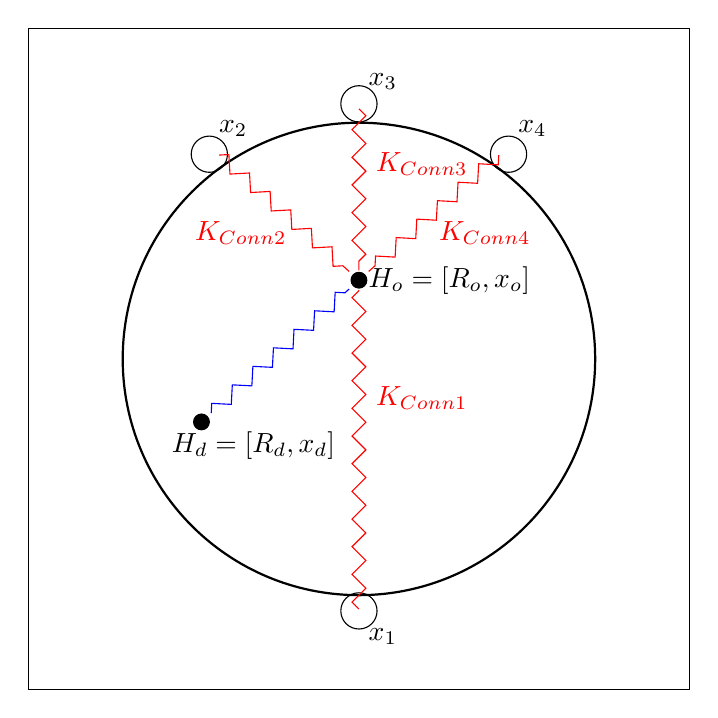
\begin{tikzpicture}
\tikzstyle{spring}=[thick,decorate,decoration={zigzag,pre length=0.3cm,post length=0.3cm,segment length=5}]
 \draw [black] (0.8,0.8) rectangle (9.2,9.2);
  \draw [black, thick] (5,5) circle [radius=3];
 \node (x3) at (5,8.3){} ;
   \node (x1)at (5,1.7){} ;
    \node (x2) at (3.1,7.7){} ;
     \node (x4) at (6.9,7.7){} ;
     \node (Ho) at (5,6){};
     \node (Hd) at (3,4.2){};
     
     \node [above right] at (5,8.3){$x_3$} ;
   \node [below right] at (5,1.7){$x_1$} ;
    \node [above right] at (3.1,7.7){$x_2$} ;
     \node [above right] at (6.9,7.7){$x_4$} ;
     \node [right]at (5,6){$H_o=[R_o,x_o]$};
     \node [below right]at (2.5,4.2){$H_d=[R_d,x_d]$};
     
     \node [red]at (5.8,4.5){$K_{Conn1}$};
     \node [red]at (3.5,6.6){$K_{Conn2}$};
     \node [red]at (5.8,7.48){$K_{Conn3}$};
     \node [red]at (6.6,6.6){$K_{Conn4}$};
     
    \draw  (5,8.24) circle [radius=0.23];
    \draw  (5,1.8) circle [radius=0.23];
     \draw  (3.1,7.6) circle [radius=0.23];
      \draw  (6.9,7.6) circle [radius=0.23];
       \draw  [fill=black] (5,6) circle [radius=0.1];
       \draw  [fill=black] (3,4.2) circle [radius=0.1];
      
      \draw[red,decorate,decoration=zigzag] (x3) -- (Ho);
      \draw[red,decorate,decoration=zigzag] (x1) -- (Ho);
      \draw[red,decorate,decoration=zigzag] (x2) -- (Ho);
      \draw[red,decorate,decoration=zigzag] (x4) -- (Ho);
       \draw[blue,decorate,decoration=zigzag] (Hd) -- (Ho);
%  \draw [gray] (6,0) arc [radius=1, start angle=45, end angle= 120]; 
%   \pszigzag[coilheight=0.5](0,0)(3.5,0)
%       \uput*[0](3.5,0){0.50}
 \end{tikzpicture}

%\begin{tikzpicture}[M1/.style={rectangle,draw=black,minimum size=2cm,thick}]
%
%    \tikzstyle{spring}=[thick,decorate,decoration={zigzag,pre length=0.3cm,post length=0.3cm,segment length=5}]
%    \tikzstyle{ground}=[fill,pattern=north east lines,draw=none,minimum width=0.75cm,minimum height=0.3cm]
%    \node [M1] (M1) {};
%    \node (wall1) [ground, minimum width=3cm,yshift=-3cm] {};
%    \draw (wall1.north west) -- (wall1.north east);
%    \draw [spring] (wall1.170) -- ($(M1.south east)!(wall1.170)!(M1.south west)$) node[pos=.5,left] {$k_2$};
%    \draw [spring] (wall1.10) -- ($(M1.south west)!(wall1.10)!(M1.south east)$) node[pos=.5,right] {$k_3$};
%    \node (wall2) [ground, minimum width=3cm,yshift=3cm] {};
%    \draw (wall2.south west) -- (wall2.south east);
%    \draw [spring] (wall2.170) -- ($(M1.north east)!(wall2.170)!(M1.north west)$) node[pos=.5,left] {$k_1$};
%    \draw [-latex,thick] (1.5,0) -- (1.5,1) node [pos=.5,right] {$x$};
%    \filldraw circle (.05) node [pos=.5,below] {\tiny $CG$};
%    \node [rotate=90,above] at (M1.west) {Mass,$m$};
%    \node at (0,-3.5) {(a)};
%        \begin{scope}[xshift=5cm]
%            \node [M1] (M1) {};
%            \node (wall1) [ground, minimum width=3cm,yshift=-3cm] {};
%            \draw (wall1.north west) -- (wall1.north east);
%            \draw [spring] (wall1) -- ($(M1.south east)!(wall1)!(M1.south west)$) node[pos=.5,left] {$k_2^*$};
%            \node (wall2) [ground, minimum width=3cm,yshift=3cm] {};
%            \draw (wall2.south west) -- (wall2.south east);
%            \draw [spring] (wall2) -- ($(M1.north east)!(wall2)!(M1.north west)$) node[pos=.5,left] {$k_1$};
%            \draw [-latex,thick] (1.5,0) -- (1.5,1) node [pos=.5,right] {$x$};
%            \filldraw circle (.05) node [pos=.5,below] {\tiny $CG$};
%            \node [rotate=90,above] at (M1.west) {Mass,$m$};
%            \node at (0,-3.5) {(b)};
%        \end{scope}
%\end{tikzpicture}
%
%\begin{tikzpicture}
%\node  (image) {\fbox{\includegraphics[width=0.25\textwidth]{initial_posture_croped}}};
%\end{tikzpicture}
%
%
%
%\begin{pspicture}(0,-4)(5,5)
% \pszigzag(0,4)(3.5,4) { \psset{linewidth=0.2pt}
%  \psline[arrowscale=2,tbarsize=3mm]{|<->|}(4.5,3.5)(4.5,4.5) 
%  \psline[linestyle=dashed](2.5,4.5)(4.5,4.5)
%   \psline[linestyle=dashed](2.75,3.5)(4.5,3.5)
%    \psline[arrowscale=2,tbarsize=3mm]{|<->|}(1.75,3.2)(2.75,3.2)
%     \uput[-90](2.15,3){\footnotesize\texttt{coilheight$\times$coilwidth}} } 
%    \uput*[0](3.5,4){coilwidth}
%     \pszigzag[coilheight=0.75](0,1.5)(3.6,1.5) 
%     \uput*[0](3.5,1.5){0.75}
%      \pszigzag[coilheight=0.5](0,0)(3.5,0)
%       \uput*[0](3.5,0){0.50}
%        \pszigzag[coilheight=1.25](0,-1.5)(3.5,-1.5) 
%        \uput*[0](3.5,-1.5){1.25} 
%        \pszigzag*[coilheight=0.5](0,-3)(3.5,-3) 
%        \uput*[0](3.5,-3){0.50}
%\end{pspicture}
%\end{document}}
   		\caption{Τα ακροδάκτυλα $x=[x_1,x_2,x_3,x_4]^T$ συγκρατούν σφαιρικό--κυλινδρικό αντικείμενο με τα εικονικά ελατήρια που διαμορφώνουν τον έλεγχο όπως περιγράφεται στη σχέση \eqref{eq:Potentials_Definitions}}
   		\label{fig:IPC_Virtual_Linkages}
\end{figure}
\newpage
Στη συνέχεια παρουσιάζουμε αναλυτικά τον τρόπο με τον οποίο υπολογίζονται οι μερικές παράγωγοι των επιμέρους δυναμικών ως προς τη γωνία των αρθρώσεων $\theta$ για την εισαγωγή τους στο σχήμα ελέγχου ξεκινώντας από το δυναμικό της ακαμψίας της περιστροφικής κίνησης. \\




\subsection{Περιστροφική Ακαμψία}

Η σχέση της παραγώγου αυτής με τη μερική παράγωγο $\frac{\partial V_{o,r}(\theta)}{\partial \theta}$ είναι η ακόλουθη,
\begin{equation}
\dot{V}_{o,r}(\theta)=\dot{\theta}^T\frac{\partial V_{o,r}(\theta)}{\partial \theta}.\label{eq:rotational_potential_time_derivative_partial_derivative}
\end{equation}
Παραγώγιση στο χρόνο του δυναμικού $V_{o,r}$ όπως ορίστηκε στην \eqref{eq:rotational_potential} δίνει,
\begin{equation}
\dot{V}_{o,r}(\theta)=4\epsilon^T_bK_{o,r}\dot{\epsilon}_b. \label{eq:rotational_potential_time_derivative}
\end{equation}
Aπό το ρυθμό μεταβολής του κουατέρνιου $\dot{\epsilon}_b$ μπορούμε να πάρουμε τη σχέση που δίνει την αντίστοιχη γωνιακή ταχύτητα $\omega_o$ του πλαισίου. Η σχέση που επιτελεί αυτή την διαφορική αντιστοίχηση είναι η ακόλουθη,
\begin{equation}
\dot{\epsilon}_b = J_{\omega\epsilon}(\theta)\omega_o \label{eq:quaternion_rate}
\end{equation}

Η μετατροπή από ένα πίνακα στροφής $R$ στο αντίστοιχο quaternion $\epsilon=[\epsilon_0\phantom{1} (\epsilon_{b1}\phantom{1}\epsilon_{b3}$\\$\phantom{1}\epsilon_{b3})]$ δεν είναι μονοσήμαντη και γίνεται χρήση ειδικού αλγορίθμου επιλογής της κατάλληλης σχέσης κάθε φορά ανάλογα με τις τιμές των στοιχείων του πίνακα στροφής~\cite{Diebel:2006fk}. 
Η Ιακωβιανή μήτρα $J_{\omega\epsilon}(\theta)$ είναι~\cite{Diebel:2006fk},
\begin{equation}
J_{\omega\epsilon}(\theta)=\frac{1}{2}
\begin{bmatrix}
\epsilon_0 &-\epsilon_3 &\epsilon_2\\
\epsilon_3 &\epsilon_0 &-\epsilon_1\\
-\epsilon_2 &\epsilon_1 &\epsilon_0\\   
\end{bmatrix}^T
\end{equation}
Για τη γωνιακή ταχύτητα του πλαισίου ισχύει η ακόλουθη σχέση,
\begin{equation}
[\omega_o \times]=R_o^T\dot{R}_o \label{eq:omega_skew}
\end{equation}
Αναπτύσουμε το δεύτερο όρο με το κανόνα της αλυσίδας (chain rule) έτσι ώστε να προκύψουν διακριτά οι διαφορικοί κινηματικοί συσχετισμοί μεταξύ εικονικού πλαισίου -- ακροδακτύλων και ακροδακτύλων -- αρθρώσεων,
\begin{equation}
\dot{R}_o =  \frac{\partial R_o}{\partial x^T}\frac{\partial x}{\partial \theta^T}\dot{\theta}
\end{equation}
ο όρος $\frac{\partial R_o}{\partial x^T}$ μπορεί εύκολα να υπολογισθεί παραγωγίζοντας τις \eqref{eq:r1_unit} \eqref{eq:r3_unit} \eqref{eq:r2_unit} μερικώς ως προς το διάνυσμα $x^T$. Ο όρος $\frac{\partial x}{\partial \theta^T}$ είναι η Ιακωβιανή μήτρα του χεριού $J_{H} = \frac{\partial x}{\partial \theta^T}$\eqref{eq:Hand_Jacobian}.
Τελικά έχουμε 
\begin{equation}
\omega_o=J_{o,r}(\theta)\dot{\theta}. \label{eq:jacobian_omega}
\end{equation}
%με
%\begin{equation}
%J_{o,r}(\theta)\dot{\theta}=
%\begin{bmatrix}
%R_o^T \frac{\partial R_o}{\partial x^T}\frac{\partial x}{\partial \theta^T}\times^{}
%\end{bmatrix}
%\end{equation}
Με αντικατάσταση στην \eqref{eq:quaternion_rate} και στη συνέχεια στην \eqref{eq:rotational_potential_time_derivative} έχουμε
\begin{equation}
\dot{V}_{o,r}(\theta)=\dot{\theta}^TJ^T_{o,r}4J^T_{\omega\epsilon}K_{o,r}\epsilon_b \label{eq:final_rotational_potential_time_derivative}
\end{equation}
και από \eqref{eq:rotational_potential_time_derivative_partial_derivative} και \eqref{eq:final_rotational_potential_time_derivative} προκύπτει τελικά,
\begin{equation}
\frac{\partial V_{o,r}(\theta)}{\partial \theta}=J^T_{o,r}4J^T_{\omega\epsilon}K_{o,r}\epsilon_b \label{eq:rotational_term}
\end{equation}
\\

\subsection{Ακαμψία Γραμμικής Μετατόπισης}

Αυτή τη φορά παραγωγίζουμε τον όρο δυναμικού της γραμμικής μετατόπισης \eqref{eq:translational_potential} ως προς το χρόνο και έχουμε,
\begin{equation}
\dot{V}_{o,t}(\theta)=(x_o-x_{o,des})^TR_oK_{o,t}\frac{d}{dt}\{R_o^T(x_o-x_{o,des}) \label{eq:translational_potential_time_derivative}\}
\end{equation}
Αναπτύσουμε τον όρο $\frac{d}{dt}\{R_o^T(x_o-x_{o,des})\}$,
\begin{equation}
\frac{d}{dt}\{R_o^T(x_o-x_{o,des})\}=\dot{R}_o^T(x_o-x_{o,des})+R_O^T\frac{\partial x_o}{\partial x^T}\frac{\partial x^T}{\partial \theta^T}\dot{\theta}
\end{equation}
από \eqref{eq:omega_skew}\eqref{eq:jacobian_omega} σε συνδιασμό με τις ιδιότητες των συμμετρικών πινάκων στροφής $[v\times]^T=-[v\times]$, $[v\times]w=-[w\times]v$ βγαίνει κοινός παράγοντας η γωνιακή ταχύτητα των αρθρώσεων  $\dot{\theta}$
\begin{equation}
\frac{d}{dt}\{R_o^T(x_o-x_{o,des})\} = [[(R_o^T(x_o-x_{o,des}))\times]J_{o,r}+R_O^T\frac{\partial x_o}{\partial x^T}\frac{\partial x^T}{\partial \theta^T}]\dot{\theta}
\end{equation}
Η μερική παράγωγος της θέσης του πλαισίου ως προς τις θέσεις των ακροδακτύλων από την \eqref{eq:frame_position} $\frac{\partial x_o}{\partial x^T}=\frac{1}{N}I_{3N\times3}$ και $\frac{\partial x^T}{\partial \theta^T}$ είναι η ιακωβιανή μήτρα του χεριού $J_{H} = \frac{\partial x}{\partial \theta^T}$. Τελικά λοιπόν η παράγωγος του δυναμικού της γραμμικής μετατόπισης είναι,
\begin{equation}
\dot{V}_{o,t}(\theta)=\dot{\theta}^TJ^T_{o,t}K_{o,t}R^T_o(x_o-x_{o,des})
\end{equation}
απ' όπου προκύπτει η μερική παράγωγος που είναι και ο όρος που θα προστεθεί στο σήμα ελέγχου της ροπής στις αρθρώσεις είναι,
\begin{equation}
\frac{\partial V_{o,t}(\theta)}{\partial \theta}=J^T_{o,t}K_{o,t}R^T_o(x_o-x_{o,des}) \label{eq:translational_term}
\end{equation}
με 
\begin{equation}
J_{o,t} = [\frac{1}{N}J_{H}^T I_{3N\times 3}R_o -  J_{o,r}^T([(R_o^T(x_o-x_{o,des})\times])^T \label{eq:Translational_Jacobian_to_Vframe}
\end{equation}

Αθροίζοντας τις \eqref{eq:translational_term} \eqref{eq:rotational_term} ουσιαστικά διαμορφώνεται στο χώρο ένα ελατήριο 6 διαστάσεων, ως προς τις γραμμικές και περιστροφικές μετατοπίσεις, συσχετιζόμενο με το αντικείμενο. 
\\


\subsection{Συνδετική Ακαμψία}

Για τον έλεγχο των εσωτερικών δυνάμεων (grasping forces) ορίζονται εικονικά ελατήρια μεταξύ ακροδακτύλων $x_i$ και της θέσης $x_o$ του εικονικού πλαισίου με ρυθμιζόμενο το σημείο ισορροπίας αυτών $l_{i,des}$ έτσι ώστε να ικανοποιούνται οι περιορισμοί των τριβών (βλ σχήμα \ref{eq:Potentials_Definitions}).

Το εικονικό δυναμικό για τον όρο της συνδετικής ακαμψίας διαμορφώνεται σφαιρικά συμμετρικά ως προς τα ακροδάκτυλα,
\begin{equation}
V_{conn}(\theta)=\frac{1}{2}\sum_{i=1}^{N}K_{conn,i}[||\Delta x_i|| - l_{i,des} ]^2
\end{equation}
όπου $\Delta x_i = x_i - x_o$ και $K_{conn,i}$ η αντίστοιχη ακαμψία επιλέγεται πάντα θετική. Παραγωγίζοντας μερικώς ως προς τη γωνιακή θέση των αρθρώσεων $\theta$ έχουμε,
\begin{equation}
\frac{\partial V_{Conn}(\theta)}{\partial \theta} = J_H^T \sum_{i=1}^{N}[\frac{\partial \Delta x_i^T}{\partial x}\frac{K_{conn,i}(||\Delta x_i|| - l_{i,des})}{||\Delta x_i||}\Delta x_i ]  
\end{equation}
η μερική παράγωγος $\frac{\partial \Delta x_i^T}{\partial x}$ υπολογίζεται,
\begin{equation} 
\begin{matrix}
\frac{\partial \Delta x_1^T}{\partial x} =  [(1-\frac{1}{N})I_{3\times3}\quad(-\frac{1}{N})I_{3\times3}\quad\dots\quad(-\frac{1}{N})I_{3\times3}]
\\
\frac{\partial \Delta x_2^T}{\partial x} =  [(-\frac{1}{N})I_{3\times3}\quad(1-\frac{1}{N})I_{3\times3}\quad\dots\quad(-\frac{1}{N})I_{3\times3}]\\
\vdots\\
\frac{\partial \Delta x_N^T}{\partial x} =  [(\underset{\text{\normalsize1}}{-\frac{1}{N})I_{3\times3}}\quad \underset{\text{\normalsize 2}}{(-\frac{1}{N})I_{3\times3}}\quad\dots\quad \underset{\text{\normalsize N}}{(1-\frac{1}{N})I_{3\times3}]}\\
\end{matrix}
\end{equation}
τελικά ο όρος της συνδετικής ακαμψίας γράφεται πιο κομψά σε μορφή πινάκων ως εξής,
\begin{equation}
\frac{\partial V_{Conn}(\theta)}{\partial \theta}=J^T_{conn}K_{Conn}   \begin{bmatrix} % or pmatrix or bmatrix or Bmatrix or ...
      ||\Delta x_1|| - l_{1,des} \\
      \vdots\\
      ||\Delta x_N|| - l_{N,des}
   \end{bmatrix}
\end{equation}
με,
\begin{equation}
J^T_{Conn}=J_H^T\begin{bmatrix}
\frac{\partial \Delta x_1^T}{\partial x} \frac{\Delta x_1}{||\Delta x_1||}\phantom{1}\dots\phantom{1} \frac{\partial \Delta x_N^T}{\partial x} \frac{\Delta x_N}{||\Delta x_N||} \label{eq:Connection_Jacobian_to_Vframe}
\end{bmatrix}
\end{equation}
και,
\begin{equation}
K_{Conn} = block diag\{K_{Conn,1}, \dots,K_{Conn,N}\}
\end{equation}
\\



\subsection{Έλεγχος Πλεοναζόντων Βαθμών Ελευθερίας}

Βάσει του μέχρι τώρα σχεδιασμού του ελεγκτή ουσιαστικά διατυπώνεται πλήρης ορισμός μόνο για τις θέσεις των ακροδακτύλων $x_i(\theta_i)$. Δεδομένου ότι η θέση $x_i$ είναι προφανώς διάνυσμα $\in \mathbb{R}^3$ και οι βαθμοί ελευθερίας του κάθε δακτύλου είναι 4 η ρομποτική διάταξη είναι κινηματικά πλεονασματική κατά 1 βαθμό ελευθερίας. 

Εκμεταλευόμενοι αυτό το γεγονός ορίζουμε υποεργασία στο μηδενικό χώρο (Null Space) του ρομποτικού δακτύλου έτσι ώστε να εισάγουμε μία σύζευξη ανθρωπομορφικού χαρακτήρα μεταξύ των δύο τελευταίων αρθρώσεων $\theta_{i3}$ και $\theta_{i4}$ με στόχο την εξασφάλιση κάθετης προβολής του ακροδακτύλου στην επιφάνεια του αντικειμένου μεγιστοποιώντας τον κώνο τριβής. 

Ο επιθυμητός έλεγχος διαμορφώνεται για πλεονασματικές διατάξεις με τον ακόλουθο τρόπο,
\begin{equation}
\tau_{d}=\tau_{d,cart}+N(\theta)\tau_{d,N}
\end{equation}
όπου $\tau_{d,cart}$, ο επιθυμητός έλεγχος στο καρτεσιανό επίπεδο των ακροδακτύλων όπως ουσιαστικά τον ορίσαμε στις αμέσως προηγούμενες ενότητες διά της ακαμψίας του εικονικού πλαισίου, $N(\theta)$ ο πίνακας προβολής στο μηδενικό χώρο της ρομποτικής λαβής και τέλος,
\begin{equation}
\tau_{d,N}=-K_N(\theta-\theta_N)-D_N\dot{\theta}
\end{equation}
ο νόμος ελέγχου PD της επιθυμητής υποεργασίας.\\

Ο πίνακας προβολής μπορεί να προκύψει στατικά,
\begin{equation}
N(\theta)=V(\theta)^TV(\theta)
\end{equation}
όπου για τον πίνακα $V(\theta)$ ισχύει, 
\begin{equation}
V(\theta)J_Η^T(\theta)=0
\end{equation} 
Ο $V(\theta)$ αποτελεί ουσιαστικά έναν πίνακα μηδενισμού της Ιακωβιανής μήτρας και μπορεί να υπολογιστεί πρακτικά με ανάλυση της Ιακωβιανής σε ιδιάζουσες μορφές. Πρακτικά προκύπτει ότι αυτού του τύπου στατική ανάλυση για τη προβολή στο μηδενικό χώρο της Ιακωβιανής επηρεάζει τελικά το καρτεσιανό χώρο του στοιχείου δράσης~\cite{Alin-Albu-Schaffer:2003fk}. Προκειμένου να λάβουμε δυναμικά συνεπή συμπεριφορά μεταφέρουμε αρχικά τη δυναμική εξίσωση \eqref{eq:hand_dynamic_equation} του ρομποτικού χεριού από το χώρο των αρθρώσεων στο χώρο των ακροδακτύλων. Για τη ταχύτητα των ακροδακτύλων καθώς και για την επιτάχυνση ισχύει,
\begin{equation}
\dot{x}=J(\theta)\dot{\theta} \label{eq:Jacobian_velocities}
\end{equation}
\begin{equation}
\ddot{x}=J(\theta)\ddot{\theta}+\dot{J}(\theta)\dot{\theta}  \label{eq:Jacobian_accelerations}
\end{equation}
Με αντικατάσταση στην \eqref{eq:hand_dynamic_equation}  έχουμε,
\begin{equation}
\ddot{x}-\dot{J}(\theta)\dot{\theta}+J(\theta)M^{-1}(\theta)(C(\theta,\dot{\theta})\dot{\theta}+g(\theta))=J(\theta)M^{-1}(\theta)\tau_d \label{eq:Dynamics_Equation_Coordinates_Transformation}
\end{equation}
έτσι λοιπόν προκύπτει εύλογα ότι για την εξασφάλιση δυναμικά συνεπούς ελέγχου στο μηδενικό χώρο ο πίνακας προβολής πρέπει να εξασφαλίζει,
\begin{equation}
J(\theta)M(\theta)^{-1}N(\theta)=0
\end{equation}
τελικά η λύση που χρησιμοποιούμε για το δυναμικό πίνακα προβολής στο μηδενικό χώρο~\cite{O.Khatib:1987uq},
\begin{equation}
N(\theta)=(I-J^T(\theta)\Lambda(\theta)J(\theta)M^{-1}(\theta))
\end{equation}
όπου,
\begin{equation}
\Lambda(\theta)=(J(\theta)M^{-1}(\theta)J(\theta)^T)^{-1}
\end{equation}

%\begin{equation}
%\tau_{red}=(I-J^+J)\xi
%\end{equation}
%όπου $J^+$ η ψευδοανάστροφη μήτρα Moore $J^+=J^T(JJ^T)^{-1}$ και 
%$\xi$ η κλίση του δυναμικού που περιγράφει την επιθυμητή υποεργασία μέσω ελάττωσης αυτού,
%\begin{equation}
%\xi=k_r\frac{\partial V_{red}}{\partial \theta}
%\end{equation}
%Όπου $k_r$ το κέρδος του αναλογικού ελεγκτή πλεονάζοντων βαθμών ελευθερίας. Το δυναμικό επιλέγεται έτσι ώστε να επιτευχθεί σύζευξη των $\theta_{i3}$ και $\theta_{i4}$ με τον ακόλουθο τρόπο,
Ο νόμος ελέγχου στο μηδενικό χώρο σχεδιάζεται, όπως προείπαμε για τη σύζευξη των δύο τελευταίων βαθμών ελευθερίας, με τον ακόλουθο τρόπο, 
%\begin{equation}
%V_{i,red}=\frac{1}{2}(\theta_{i3}-\alpha\theta_{i4})^2
%\end{equation}
\begin{equation}
\tau_{d,N}=-K_{Null}(\theta_{i3}-\alpha\theta_{i4})-D_{Null}\dot{\theta}
\end{equation}
όπου $\alpha\in[0,1]$ ο συντελεστής με τον οποίο μπορούμε να ρυθμίσουμε τη σχέση της σύζευξης μεταξύ των $\theta_{i3}$ και $\theta_{i4}$.
\\

\subsection{Σχεδιασμός Όρου Απόσβεσης}

Προκειμένου να καθοριστεί και η μεταβατική συμπεριφορά του συστήματος σχεδιάζεται ο δυναμικός όρος απόσβεσης $D(\theta)$ του ελεγκτή βάσει της ακόλουθης μεθοδολογίας~\cite{Alin-Albu-Schaffer:2003fk,Alin-Albu-Schaffer:2004kx,WimboeckOttHirzinger2006}. \\

Αρχικά βάσει των διαφορικών αντιστοιχίσεων μεταξύ των γωνιακών ταχυτήτων των αρθρώσεων $\dot{\theta}$ και των ταχυτήτων των μεταβλητών στο χώρο εργασίας $\dot{x}_o$, $\omega_o$, $||\Delta\dot{x}||$ όπως περιγράφονται από τις σχέσεις   \eqref{eq:Translational_Jacobian_to_Vframe} \eqref{eq:jacobian_omega} \eqref{eq:Connection_Jacobian_to_Vframe} αντίστοιχα, μπορούν να ομαδοποιηθούν αυτοί οι διαφορικοί συσχετισμοί με τον ακόλουθο τρόπο,
\begin{equation}
\underbrace{\begin{bmatrix} % or pmatrix or bmatrix or Bmatrix or ...
      \dot{x}_o \\
      \omega_{o,0} \\
      ||\Delta \dot{x}||
   \end{bmatrix}}_{\dot{\overline{x}}} = \underbrace{ \begin{bmatrix} % or pmatrix or bmatrix or Bmatrix or ...
         J_{o,t} \\
         J_{o,r}\\
         J_{conn}
      \end{bmatrix}}_{J_{tot}}\dot{\theta}
\end{equation}
ορίζοντας το $\dot{\overline{x}} \in \mathbb{R}^{6+N}$ το γενικευμένο διάνυσμα διαφορικών συντεταγμένων και $J_{tot}$ η συμπτυγμένη Ιακωβιανή μήτρα.\\

Στις εξισώσεις, \eqref{eq:Jacobian_velocities} \eqref{eq:Jacobian_accelerations} \eqref{eq:Dynamics_Equation_Coordinates_Transformation}, βλέπουμε το μετασχηματισμό του δυναμικού μοντέλου του χεριού από το χώρο των γωνιών των αρθρώσεων στον καρτεσιανό χώρο μεταβλητών θέσης. Στη προκειμένη περίπτωση θεωρώντας το  $\overline{x}$ ως τις γενικευμένες μεταβλητές θέσης του συστήματος της ρομποτικής λαβής μετασχηματίζουμε αντίστοιχα και έχουμε, 
\begin{equation}
\ddot{\overline{x}}-\dot{J_{tot}}(\theta)\dot{\theta}+J_{tot}(\theta)M^{-1}(\theta)(C(\theta,\dot{\theta})\dot{\theta}+g(\theta))=J_{tot}(\theta)M^{-1}(\theta)\tau 
\end{equation}
Με τον νόμο ελέγχου όπως τον έχουμε ορίσει για το σύστημα βάσει των σχέσεων \eqref{eq:control_law_tau} \eqref{eq:rotational_term} \eqref{eq:Connection_Jacobian_to_Vframe} έχουμε,
\begin{equation}
\ddot{\overline{x}}-\dot{J_{tot}}(\theta)\dot{\theta}+J_{tot}(\theta)M^{-1}(\theta)(C(\theta,\dot{\theta})\dot{\theta}+g(\theta))=J_{tot}(\theta)M^{-1}(\theta)(-D(\theta)\dot{\theta}-\frac{\partial V_d}{\partial \theta}(\theta)+g(\theta))
\end{equation}
και ορίζοντας την ακόλουθη σχέση μεταξύ της απόσβεσης του χώρου των αρθρώσεων στο χώρο των γενικευμένων συντεταγμένων του χώρου εργασίας, 
\begin{equation}
D(\theta)=J_{tot}^TD_{\overline{x}}(\theta)J_{tot}
\end{equation}
έχουμε τελικά,
\begin{equation}
\ddot{\overline{x}}-\dot{J_{tot}}(\theta)\dot{\theta}+J_{tot}(\theta)M^{-1}(\theta)(C(\theta,\dot{\theta})\dot{\theta})=J_{tot}(\theta)M^{-1}J_{tot}^T(\theta)(-D_{\overline{x}}\dot{\overline{x}}-F_{\overline{x}}) \label{eq:dynamics_closed_system}
\end{equation}
όπου $F_{\overline{x}}=[f_o\phantom{1} m_o \phantom{1} f_{Conn}]^T=K_{\overline{x}}(\overline{x}-\overline{x}_{des})=K_{\overline{x}}e_{\overline{x},o}$ με $K_{\overline{x}}=blockdiag\{K_{o,t}\phantom{1} K_{o,r} \phantom{1} K_{Conn} \}$.  

Για λόγους απλότητας λαμβάνονται υπ' όψη μόνο τα γνήσια αδρανειακά φαινόμενα 2ης τάξης για το σχεδιασμό του δυναμικού πίνακα απόσβεσης, παραλείποντας δηλαδή τους όρους Coriolis οι οποίοι περιλαμβάνουν τα γινόμενα μεταξύ γωνιακών ταχυτήτων. H προηγούμενη σχέση \eqref{eq:dynamics_closed_system} απλοποιείται ακολούθως, 
\begin{equation}
M_{H,\overline{x}}(\theta)\ddot{\overline{x}}=-D_{\overline{x}}\dot{\overline{x}}-F_{\overline{x}}
\end{equation}
όπου,
\begin{equation}
M_{H,\overline{x}}(\theta)=(J_{tot}M(\theta)^{-1}J^T_{tot})^{-1} \label{eq:generalized_hand_coordinates_inertia}
\end{equation}
Σε αυτό το σημείο μπορούμε να εισάγουμε και τη δυναμική επίδραση του αντικειμένου, $F_o=M_o[\ddot{x}_o\phantom{1} \dot{\omega_o}\phantom{1} O_{N\times6}]^T$ (θεωρούμε ότι η βαρυτική δύναμη του αντικειμένου αντισταθμίζεται όπως εξηγούμε αναλυτικά στην επόμενη ενότητα), ως εξωτερική δύναμη, οπότε και έχουμε,
\begin{equation}
M_{H,\overline{x}}(\theta)\ddot{\overline{x}}=-D_{\overline{x}}\dot{\overline{x}}-F_{\overline{x}}-F_o
\end{equation}
και τελικά,
\begin{equation}
M_{\overline{x}}(\theta)\ddot{\overline{x}}=-D_{\overline{x}}\dot{\overline{x}}-F_{\overline{x}} \label{eq:dynamics_object_level}
\end{equation}
όπου,
\begin{equation}
M_{\overline{x}}(\theta)=M_{H,\overline{x}}(\theta)+   \begin{bmatrix} % or pmatrix or bmatrix or Bmatrix or ...
      I_{6\times 6} \\
      0_{N\times 6} \\
   \end{bmatrix}M_o [I_{6\times 6}, 0_{6\times N}]
\end{equation}
Η δυναμική του λάθους παρακολούθησης τροχιάς προκύπτει βάσει της \eqref{eq:dynamics_object_level} για μηδενικές εξωτερικές δυνάμεις, 
\begin{equation}
M_{\overline{x}}(\theta)\ddot{e_{\overline{x},o}}+D_{\overline{x}}\dot{e_{\overline{x},o}}+K_{\overline{x}}e_{\overline{x},o}=0
\end{equation}

Σε αυτό το σημείο ο όρος απόσβεσης επιλέγεται ως συνάρτηση της μήτρας αδράνειας $M_{\overline{x}}$ και του αναλογικού κέρδους $K_{\overline{x}}$ έτσι ώστε να προκύπτει δυναμικά συνεπής απόσβεση για όλες τις δυνατές θέσεις της διάταξης. 

Βάσει της μεθοδολογίας της διπλής διαγωνοποίησης της θεωρίας της γραμμικής άλγεβρας προκύπτει ότι για ένα θετικά ορισμένο συμμετρικό πίνακα $n\times n$ $M_{\overline{x}}$ και για ένα πίνακα $K_{\overline{x}}$ συμμετρικό $n\times n$, υπάρχει πίνακας πλήρους τάξης $Q$ έτσι ώστε, $M_{\overline{x}}=QQ^T$ και  $K_{\overline{x}}=QK_{d0}Q^T$ για τυχαίο διαγώνιο πίνακα $K_{d0}$.

Επιλέγοντας τον πίνακα απόσβεσης,
\begin{equation}
D_{\overline{x}}(\theta)=2Q(\theta)D_{\xi}K_{do}^{1/2}Q(\theta)^T
\end{equation}
η δυναμική του σφάλματος παρακολούθησης τροχιάς διαμορφώνεται,
\begin{equation}
Q(\theta)Q(\theta)^Τ\ddot{e_{\overline{x},o}}+2Q(\theta)D_{\xi}K_{do}^{1/2}Q(\theta)^T\dot{e_{\overline{x},o}}+Q(\theta)K_{do}Q(\theta)^Te_{\overline{x},o}=0
\end{equation}
Βγάζοντας κοινό παράγοντα τη μήτρα $Q(\theta)$ και ανάγοντας το σύστημα ως προς στο νέο χώρο γενικευμένων μεταβλητών $w=Q^T(\theta)e_{\overline{x},o}$ προκύπτει η επιθυμητή συμπεριφορά συστήματος,
\begin{equation}
\ddot{w}+2D_{\xi}K_{do}^{1/2}\dot{w}+K_{do}w=0
\end{equation}

  
Προκύπτει ότι τα στοιχεία της διαγωνίου της μήτρας αδράνειας $M_{\overline{x}}$ είναι τα κυρίαρχα επηρεάζοντας ουσιαστικά τα αδρανειακά χαρακτηριστικά του συστήματος. Λαμβάνοντας υπόψη λοιπόν μόνο τα διαγώνια στοιχεία έχουμε, 
\begin{equation}
M_{\overline{x}}(\theta)=(blockdiag\{diag\{J_{tot}M(\theta)^{-1}J^T_{tot}\}\})^{-1} +   \begin{bmatrix} % or pmatrix or bmatrix or Bmatrix or ...
      I_{6\times 6} \\
      0_{N\times 6} \\
   \end{bmatrix}M_o [I_{6\times 6}, 0_{6\times N}]
\end{equation}
Οπότε επιλέγεται ουσιαστικά, $Q(\theta)=\sqrt{M_{\overline{x}}}$.

Τελικά ο όρος της απόσβεσης που καθορίζει τη ματαβατική δυναμική συμπεριφορά του κλειστού συστήματος επιλέγεται ορίζοντας τα ακόλουθα διαγώνια στοιχεία
% έτσι ώστε η σταθερά απόσβεσης του κλειστού συστήματος $\zeta$ να είναι 
%\begin{equation}
%\zeta=\frac{1}{\xi}
%\end{equation}
\begin{equation}
D_{\overline{x},ii}(\theta)=2\xi_i\sqrt{M_{\overline{x},ii}(\theta)K_{\overline{x},ii}}
\end{equation}
όπου $\xi_i \in [0,1]$, ο επιθυμητός παράγωντας της απόσβεσης για την αντίστοιχη γενικευμένη μεταβλητή $\overline{x}_i$ και $K_{\overline{x},ii}$ τα διαγώνια στοιχεία της μήτρας των κερδών $K_{\overline{x}}=blockdiag\{K_{o,t},K_{o,r},K_{Conn}\}$. 


\section{Επεκτάσεις--Τροποποιήσεις του Ελεγκτή Εμπέδησης στο επίπεδο του αντικειμένου}

Ο έλεγχος των εσωτερικών δυνάμεων της λαβής με βάση το σχήμα συνδετικής ακαμψίας $V_{Conn}$ όπως περιγράφηκε στη προηγούμενη υποενότητα δίνει ικανοποιητικές επιδόσεις και εύρωστη--ευσταθή λαβή~\cite{WimboeckOttHirzinger2006,WimbockOttHinzinger2007,WimbockOttSchafferHirzinger}. Ιδιαίτερα εντυπωσιακό αν αναλογιστεί κανείς ότι ουσιαστικά το σύστημα είναι "τυφλό" καθώς δε βασίζεται σε κανενός είδους αισθητηριακή πληροφόρηση (force--sensor--tactile) με μόνη παραδοχή ότι τα αντικείμενα υπό χειρισμό θα προσεγγίζουν κανονικές τρισδιάστατες γεωμετρίες.\\

Η κριτική που μπορεί κανείς να ασκήσει στο συγκεκριμένο σχήμα ελέγχου των εσωτερικών δυνάμεων αποτελείται από δύο βασικούς άξονες,
\begin{itemize}
\item
Ιδιαίτερα αυξημένες απαιτήσεις από τον κώνο τριβής της επαφής στη περίπτωση χειρισμού αντικειμένου με επίπεδες επιφάνειες όπως φαίνεται και στο σχήμα~\ref{fig:contact_pressure} καθώς η κατεύθυνση του εικονικού ελατηρίου $V_{Conn,i}$ τείνει σε εφαπτομενικές ως προς την επιφάνεια του αντικειμένου διευθύνσεις.
\item
Πρακτικά δύσκολη η ρύθμιση των σημείων ισορροπίας $l_{i,des}$ για κάθε σύνδεση $V_{Conn,i}$ σε πραγματικό χρόνο για διαφορετικά αντικείμενα με αποτέλεσμα πιθανή παρουσία συνιστάμενης δύναμης στο αντικείμενο και κατά συνέπεια παρουσία τελικού σφάλματος θέσης.
\end{itemize}


\subsection{Έλεγχος Εσωτερικών Δυνάμεων βάσει Χαρακτηριστικών Επιφανείας (IPC--IF)}
\label{subsect:IPC_IF}
\begin{figure}[htbp]%  figure placement: here, top, bottom, or page
   		\centering
		%   \includegraphics[scale=0.6]{images_kefalaio3/denavit.pdf} 
   		\resizebox{0.45\textwidth}{!}{\input{images_kefalaio3/Virtual_Linkages_IPC_Rectangle_Problem.tex}}
   		\caption{Μεγάλη εφαπτομενική δύναμη ως προς την επιφάνεια του αντικειμένου στα ακροδάκτυλα $x_2$, $x_3$ από τις σφαιρικά συμμετρικές αντίστοιχες ακαμψίες $K_{Conn2}$, $K_{Conn4}$  }
   		\label{fig:contact_pressure}
\end{figure}


Βασικό επιχείρημα στη προσέγγισή μας είναι ότι σε πραγματικές ολοκληρωμένες ρομποτικές εφαρμογές ρομποτικών χειριστών υπάρχουν τουλάχιστον ένα ή και περισσότερα αισθητηριακά σύνολα (Δυνάμεων, Αφής, Όρασης) ικανά να μας δώσουν πληροφορία για την επιφάνεια του αντικειμένου και συγκεκριμένα για τη κάθετη στην επιφάνεια κατεύθυνση.

Έτσι λοιπόν, προτείνουμε επέκταση του Εγγενώς Παθητικού Ελεγκτή (IPC) εφαρμόζοντας έλεγχο των εσωτερικών δυνάμεων με την άσκηση δυνάμεων από τα ακροδάκτυλα με κατεύθυνση κάθετη και εσωτερική ως προς το αντικείμενο και την επιφάνειά που ορίζουν οι επαφές (IPC--IF) (βλ. σχήμα~\ref{fig:Perpendicular_Internal_Control}). 

\begin{figure}[htbp]%  figure placement: here, top, bottom, or page
   		\centering
		%   \includegraphics[scale=0.6]{images_kefalaio3/denavit.pdf} 
   		\resizebox{0.45\textwidth}{!}{\input{images_kefalaio3/Perpendicular_Internal_Control.tex}}
   		\caption{Εγγενώς Παθητικός Έλεγχος με Έλεγχο Εσωτερικών Δυνάμεων ασκώντας κάθετη πίεση στις επιφάνειες που ορίζουν οι επαφές (IPC--IF).}
   		\label{fig:Perpendicular_Internal_Control}
\end{figure}


Για τη κατάλληλη ρύθμιση αυτών των εσωτερικών δυνάμεων προτείνουμε τη προβολή στο μηδενικό χώρο της μήτρας λαβής.. \\

Κατά τη στατική ανάλυση \eqref{eq:GraspMatrix_Relative} έχουμε,
\begin{equation}
\begin{bmatrix} % or pmatrix or bmatrix or Bmatrix or ...
      R_o^T &R_o^T &R_o^T&R_o^T \\
      [r_{c1}\times]R_o^T & [r_{c2}\times]R_o^T&[r_{c2}\times]R_o^T&[r_{cN}\times]R_o^T \\
   \end{bmatrix}
  \begin{bmatrix} % or pmatrix or bmatrix or Bmatrix or ...
         F_{s1} \\
          F_{s2} \\
         F_{s2}\\
          F_{sN} \\
      \end{bmatrix}=
        \begin{bmatrix} % or pmatrix or bmatrix or Bmatrix or ...
         -f_{ext} \\
         -n_{ext}
      \end{bmatrix}   \label{eq:Static_Relational}
\end{equation}
με το διάνυσμα $r_{ci}$ να ορίζεται,
\begin{equation}
r_{ci}=\frac{x_i-x_o}{||x_i-x_o||}
\end{equation}
Οι εσωτερικές, κάθετες στο αντικείμενο δυνάμεις είναι,
\begin{equation}
F_s=nf_s \label{eq:Perpendicular_Forces}
\end{equation}
όπου $n=blockdiag\{n_1, n_2, n_3, n_4\}\in \mathbb{R}^{12\times4}$ τα μοναδιαία διανύσματα $n_i$ κάθετα στην επιφάνεια της επαφής $i$ αντίστοιχα.
Άρα έχουμε από  \eqref{eq:Static_Relational,eq:Perpendicular_Forces},
\begin{equation}
\underbrace{\begin{bmatrix} % or pmatrix or bmatrix or Bmatrix or ...
      R_o^Tn_1 &R_o^Tn_2 &R_o^Tn_3&R_o^Tn_4 \\
      [r_{c1}\times]R_o^Tn_1 & [r_{c2}\times]R_o^Tn_2&[r_{c2}\times]R_o^Tn_3&[r_{cN}\times]R_o^Tn_4 \\
   \end{bmatrix}}_{G}
 \underbrace{ \begin{bmatrix} % or pmatrix or bmatrix or Bmatrix or ...
         f_{s1} \\
          f_{s2} \\
          f_{s3}\\
          f_{s4} \\
      \end{bmatrix}}_{f_{s}} =
       \underbrace{ \begin{bmatrix} % or pmatrix or bmatrix or Bmatrix or ...
         -f_{ext} \\
         -n_{ext}
      \end{bmatrix}}_{F_{ext}}   \label{eq:GraspMatrix_Relative}
\end{equation}
όπου $G \in \mathbb{R}^{6\times4}$ η προκύπτουσα μήτρα λαβής. Από \eqref{eq:grasp_matrix_general_solution} η προβολή στο μηδενικό χώρο της $G$ θα είναι,
\begin{equation}
f_{s,Null}=\underbrace{(\mathbf{I}-[G]^{+}G)}_{G_{s,Null}}f_s
\end{equation}

Τελικά ο νόμος ελέγχου $\tau_{N}$ για τις εσωτερικές δυνάμεις διαμορφώνεται,
\begin{equation}
\tau_{N}(\theta)=J_H^T(\theta)\phantom{1}(\mathbf{I}-[G]^{+}G)f_s
\end{equation}



\subsection{Βαρυτική Αντιστάθμιση}
\label{subsec:Gravitational}
Εφόσον έχουμε ορίσει τις ακαμψίες των γραμμικών και στροφικών μετατοπίσεων ορίζοντας τη δύναμη $f_o$ και τη ροπή εμπέδησης $m_o$ μπορούμε εύκολα να επεκτείνουμε την υπάρχουσα δομή για την εισαγωγή όρων αντιστάθμισης της βαρυτικής επίδρασης μέσω του βαρυτικού διανύσματος $G=[0,0,mg]$. Η μεταφορική επίδραση της βαρύτητας ως προς το πλαίσιο $Η_ο$ θα είναι,
\begin{equation}
f_{g}=R_o^TG
\end{equation}
και η ροπή που θα ασκεί,
\begin{equation}
m_{o,g}=[r_{COG}\times]R_o^TG
\end{equation}
όπου $r_{COG}$, το διάνυσμα θέσης του κέντρου βάρους του αντικειμένου ως προς το πλαίσιο $H_{o}$.

Εισάγουμε του όρους αυτούς στις ~\eqref{eq:rotational_term}, ~\eqref{eq:translational_term} και έχουμε αντίστοιχα,
\begin{equation}
\frac{\partial V_{o,r}(\theta)}{\partial \theta}=J^T_{o,r}(\underbrace{4J^T_{\omega\epsilon}K_{o,r}\epsilon_b \label{eq:rotational_term_with_g}}_{m_o} +m_{o,g})
\end{equation}
\begin{equation}
\frac{\partial V_{o,t}(\theta)}{\partial \theta}=J^T_{o,t}(\underbrace{K_{o,t}R^T_o(x_o-x_{o,des}) \label{eq:translational_term_with_g}}_{f_o}+f_{o,g})
\end{equation}

Η προσθήκη της βαρυτικής αντιστάθμισης απεικονίζεται γραφικά στο σχήμα~\ref{fig:Perpendicular_Internal_Control_PlusGravity}.
\begin{figure}[htbp]%  figure placement: here, top, bottom, or page
   		\centering
		%   \includegraphics[scale=0.6]{images_kefalaio3/denavit.pdf} 
   		\resizebox{0.45\textwidth}{!}{\input{images_kefalaio3/Perpendicular_Internal_Control_plus_gravity.tex}}
   		\caption{Έλεγχος Εσωτερικών Δυνάμεων με κάθετη πίεση στις επιφάνειες του αντικειμένου σε συνδυασμό με τους όρους βαρυτικής αντιστάθμισης.}
   		\label{fig:Perpendicular_Internal_Control_PlusGravity}
\end{figure}

























\end{document}
